% this next line updated by emacs every time the file is saved:
\def\tsval{Time-stamp: < 07 May 2014 11:04MDT >}
%
% Yet Another Introductory Number Theory Textbook (Cryptology Emphasis Version)
%    
%    by Jonathan A. Poritz
%       jonathan.poritz@gmail.com  and  http://www.poritz.net/jonathan
%
%    Based, at the beginning, on: An Introductory Course in Number Theory
%           by Wissam Raji, for which see www.saylor.org/books
%      ... but since changed almost entirely.  Still: thank you, Raji, for the
%          starting point and the great example that you set!
%
%    Raji's version was release under the Creative Commons
%         CC BY 3.0 license, see https://creativecommons.org/licenses/by/3.0/
%
%    This version is released under a Creative Commons CC BY-SA 4.0 license
%         https://creativecommons.org/licenses/by-sa/4.0/
%
%    You are free to share and adapt this book for any purpose, even
%        commercially (that's what the CC license is about) but:
%          -- you must give appropriate credit to this author and to Wissam Raji
%          -- you must indicate in your version if you have made changes to our
%             originals, and
%          -- if you remix, transform, or build upon the material, you must
%             distribute your contributions under the same license as the
%             original
%          -- you may not apply legal terms or technological measures which
%             restrict others from doing anything the license permits.
%
%    While this is not a legal requirement, I would be happy to know if you are
%          using and/or adapting this work: please send such information to my
%          e-mail address jonathan.poritz@gmail.com  For that matter, if you
%          find typos or have suggestions of things to change or add, I would
%          be happy to hear that as well.
%
%
%
% --------------------------------------------------------------------------
% Some notes on using this TeX file:
%
%  It is standard LaTeX -- my version says
%   'This is pdfTeX, Version 3.1415926-2.4-1.40.13 (TeX Live 2012/Debian)'
%   at the start of the run.  It does use quite a few packages, but they are
%   all available from the standard 'net repositories ... in fact, I installed
%   nothing particularly for this book.
%
%  Here is how I produce the final yaintt.pdf file on my Linux box
%    (on other systems, you will know how that must be changed)
%      latex yaintt
%      bibtex yaintt
%      latex yaintt
%      latex yaintt
%      makeindex yaintt
%      latex yaintt
%      dvips -o yaintt.ps yaintt
%      ps2pdf yaintt.ps
%      view yaintt.pdf in my favorite viewer (I use 'evince')
%
%  Note you will need the following files in the directory where you do this:
%      yaintt.tex
%      refs.bib
%      by-sa.eps
%      cover_art.eps
%      dbend.eps
%      eng_freq_hist.eps
%      hamhip_freqs.eps
%      samp_Cct_hist.eps
%      Scytale.eps
%      seadk_Cct.eps
%      seadk_hamhip.eps
%      seadk_rkkrt.eps
%      
%  You should be able to customize this, or extract parts from it for your own
%    use fairly easily.  I tried to follow good, clear, TeX style: for example,
%    labels, for references to definitions, theorems, sections, etc., all
%    follow a fairly uniform naming convention which should be obvious just by
%    looking at a few.
%
%  I put all random, discursive text which is not in a theorem, definition,
%    example, or other such environment with semantic import, in a special
%    environment called 'discussion'.  That way it can all be cut out in case
%    a very stripped-down version of the book is desired.  In fact, there are
%    options, mentioned below (starting with the 'uncomment the following lines
%    to hide all proofs'), that allow all of various specific portions of the
%    text to be hidden.
%    I have used this, for example, on a final exam: I give the students a
%    portion of the final which asks for definitions, theorem statements and
%    so on, then when they hand that part in, I give them the rest, consisting
%    of calculations and proofs -- and along with those problems, I give them
%    a print-out of most of the textbook, but only the definitions and theorem
%    statements to consult as they work.  This stripped-down version can be
%    easily produced by uncommenting all of the lines below which call for
%    hiding discussion, examples, proofs, remarks, exercises, figures, preface,
%    release notes, and bibliography.
%    
%
%  Here are the customization options:
%
% uncomment the following line to hide all proofs
%\def\suppressallproofs{}
% uncomment the following line to hide all discussion
%\def\suppressalldiscussion{}
% uncomment the following line to hide all examples
%\def\suppressallexamples{}
% uncomment the following line to hide all definitions
%\def\suppressalldefinitions{}
% uncomment the following line to hide all lemmata
%\def\suppressalllemmata{}
% uncomment the following line to hide all propositions
%\def\suppressallpropositions{}
% uncomment the following line to hide all theorems
%\def\suppressalltheorems{}
% uncomment the following line to hide all exercises
%\def\suppressallexercises{}
% uncomment the following line to hide all remarks
%\def\suppressallremarks{}
% uncomment the following line to hide all corollaries
%\def\suppressallcorollaries{}
% uncomment the following line to hide all tables
%\def\suppressalltables{}
% uncomment the following line to hide all figures
%\def\suppressallfigures{}
% uncomment the following line to hide the table of contents
%\def\suppressToC{}
% uncomment the following line to hide the preface
%\def\suppressPreface{}
% uncomment the following line to hide the release notes
%\def\suppressReleaseNotes{}
% uncomment the following line to hide the index
%\def\suppressIndex{}
% uncomment the following line to hide the bibliography
%\def\suppressBibliography{}
%
%
%
\documentclass[12pt,letterpaper]{amsbook}
\usepackage[text={6in,9in},centering]{geometry}
\usepackage{wrapfig}
\usepackage{times}
\usepackage{amsthm}
\usepackage{amsmath}
\usepackage{amssymb}
\usepackage{mathrsfs}
\usepackage{mathtools}
\usepackage{amsfonts}
\usepackage{hyperref}
\hypersetup{
  hidelinks,
  pdftitle={Satu Lagi Buku Teks Pengantar Teori Bilangan},
  pdfauthor={Jonathan A. Poritz; berdasarkan karya Wissam Raji},
  pdfsubject={Edisi bahasa Indonesia dengan penekanan pada kriptologi},
  pdfkeywords={teori bilangan, kriptologi, induksi matematika},
  pdflang={id-ID}
}
\usepackage{graphicx}
\graphicspath{{assets/}}
\usepackage{float}
\usepackage{multirow}
\usepackage{afterpage}
\usepackage{environ}
\usepackage{xcolor}
\usepackage{pagecolor}
\newtheorem{theorem}{Teorema}[section]
\newtheorem{corollary}[theorem]{Akibat}
\newtheorem{lemma}[theorem]{Lema}
\newtheorem{proposition}[theorem]{Proposisi}
\newtheorem{examples}[theorem]{Contoh-contoh}
\theoremstyle{definition}
\newtheorem{definition}[theorem]{Definisi}
\newtheorem{exercise}{Latihan}
\theoremstyle{remark}
\newtheorem{remark}[theorem]{Catatan}
\newtheorem{example}[theorem]{Contoh}
\newtheorem*{WOprinciple}{Prinsip Keterurutan Baik}
\renewcommand{\proofname}{Bukti}
\renewcommand{\chaptername}{Bab}
\renewcommand{\contentsname}{Daftar Isi}
\renewcommand{\bibname}{Daftar Pustaka}
\renewcommand{\indexname}{Indeks}
\renewcommand{\figurename}{Gambar}
\renewcommand{\tablename}{Tabel}
\numberwithin{figure}{section}
\numberwithin{exercise}{section}
\numberwithin{section}{chapter}
\numberwithin{equation}{section}
\numberwithin{table}{section}
%macros for dealing with the emacs timestamp
\def\tsgutsb#1{\expandafter\tsgutsa #1\relax}
\def\tsgutsa#1 #2 #3 #4 #5 #6 #7\relax{#3 #4 #5  #6}
\def\timestamp{\tsgutsb{\tsval}}
\def\idtimestamp{07 Mei 2014 11:04 MDT}
\newcommand{\NN}{{\mathbb N}}
\newcommand{\RR}{{\mathbb R}}
\newcommand{\QQ}{{\mathbb Q}}
\newcommand{\ZZ}{{\mathbb Z}}
\newcommand{\Cc}{{\mathcal C}}
\newcommand{\Dd}{{\mathcal D}}
\newcommand{\Ee}{{\mathcal E}}
\newcommand{\Ff}{{\mathcal F}}
\newcommand{\Kk}{{\mathcal K}}
\newcommand{\Mm}{{\mathcal M}}
\newcommand{\Pp}{{\mathcal P}}
\newcommand{\ind}{\operatorname{ind}}
\newcommand{\ord}{\operatorname{ord}}
\newcommand{\lihat}[2]{\emph{lihat} #1}
\makeatletter
\ifdefined\NewCommandCopy
  \NewCommandCopy{\@@pmod}{\pmod}
\else
  \let\@@pmod\pmod
\fi
\DeclareRobustCommand{\pmod}{\@ifstar\@pmods\@@pmod}
\def\@pmods#1{\mkern4mu({\operator@font mod}\mkern 6mu#1)}
\makeatother
\newenvironment{preface}{}{}
\newenvironment{releasenotes}{}{}
\newenvironment{discussion}{}{}
\NewEnviron{killcontents}{}
\ifdefined\suppressallproofs
  \let\proof\killcontents
  \let\endproof\endkillcontents
\fi
\ifdefined\suppressallexamples
  \let\example\killcontents
  \let\endexample\endkillcontents
  \let\examples\killcontents
  \let\endexamples\endkillcontents
\fi
\ifdefined\suppressalldiscussion
  \let\discussion\killcontents
  \let\enddiscussion\endkillcontents
\fi
\ifdefined\suppressalldefinitions
  \let\definition\killcontents
  \let\enddefinition\endkillcontents
\fi
\ifdefined\suppressalltheorems
  \let\theorem\killcontents
  \let\endtheorem\endkillcontents
\fi
\ifdefined\suppressallpropositions
  \let\proposition\killcontents
  \let\endproposition\endkillcontents
\fi
\ifdefined\suppressalllemmata
  \let\lemma\killcontents
  \let\endlemma\endkillcontents
\fi
\ifdefined\suppressallexercises
  \let\exercise\killcontents
  \let\endexercise\endkillcontents
\fi
\ifdefined\suppressallremarks
  \let\remark\killcontents
  \let\endremark\endkillcontents
\fi
\ifdefined\suppressallcorollaries
  \let\corollary\killcontents
  \let\endcorollary\endkillcontents
\fi
\ifdefined\suppressalltables
  \let\table\killcontents
  \let\endtable\endkillcontents
  \let\tabular\killcontents
  \let\endtabular\endkillcontents
\fi
\ifdefined\suppressallfigures
  \let\figure\killcontents
  \let\endfigure\endkillcontents
\fi
\ifdefined\suppressPreface
  \let\preface\killcontents
  \let\endpreface\endkillcontents
\fi
\ifdefined\suppressReleaseNotes
  \let\releasenotes\killcontents
  \let\endreleasenotes\endkillcontents
\fi
\linespread{1.2}
\makeindex

\begin{document}
\newpagecolor{blue}
\frontmatter

\title{\ \vskip-7cm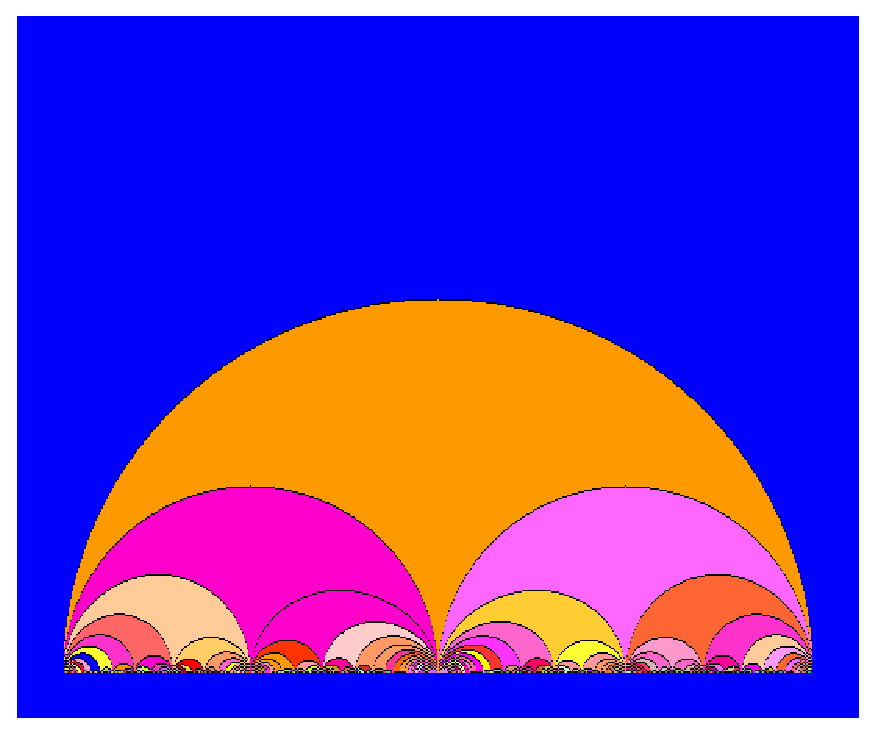
\includegraphics[width=.85\textwidth,clip]{cover_art.eps}\\\huge\color{red} Satu Lagi\\
Buku Teks Pengantar\\Teori Bilangan\\
{\Large\it (Versi dengan Penekanan pada Kriptologi)}}

\author{{\color{orange}{\Large\bf Jonathan A.~Poritz}\\{\large\it berdasarkan karya Wissam Raji}}}
\address{\color{white}\centerline{\bf Departemen Matematika dan Fisika\hphantom{XXXXX}}
\centerline{\bf Colorado State University, Pueblo}
\centerline{\bf 2200 Bonforte Blvd.}
\centerline{\bf Pueblo, CO 81001, USA}
\centerline{{\bf Surel: jonathan.poritz@gmail.com}}
\centerline{{\bf Situs web: www.poritz.net/jonathan}}
\vskip3.5cm\hfill\tiny\idtimestamp}

\maketitle
\restorepagecolor

\begin{preface}
\chapter*{Prakata}

Ini adalah draf pertama sebuah buku ajar teori bilangan tingkat sarjana yang
bebas (dalam arti kebebasan berbicara, bukan gratis seperti bir gratis,
\cite{stallman2002free}), meskipun buku ini juga tersedia secara gratis. Buku
ini digunakan dalam mata kuliah Math 319 di Colorado State University --
Pueblo pada semester musim semi 2014. Ucapan terima kasih disampaikan kepada
para mahasiswa di kelas tersebut -- Megan Bissell, Tennille Candelaria, Ariana
Carlyle, Michael Degraw, Daniel Fisher, Aaron Griffin, Lindsay Harder, Graham
Harper, Helen Huang, Daniel Nichols, dan Arika Waldrep -- yang memberikan banyak
saran berguna dan menemukan banyak salah ketik. Saya juga berterima kasih
kepada para mahasiswa dalam mata kuliah Math 242 Pengantar Pemrograman
Matematika pada semester musim semi 2014 yang sama -- Stephen Ciruli, Jamen
Cox, Graham Harper, Joel Kienitz, Matthew Klamm, Christopher Martin, Corey
Sullinger, James Todd, dan Shelby Whalen -- karena berbagai proyek pemrograman
mereka menghasilkan kode yang saya adaptasi untuk membuat beberapa gambar dan
contoh dalam buku ini.

Penulis menyampaikan penghargaan dan terima kasih atas karya {\bf An
Introductory Course in Elementary Number Theory} oleh Wissam Raji [lihat
  \href{https://www.saylor.org/books/}{Saylor Academy}], yang menjadi sumber
adaptasi awal buku ini. Karya
Raji diterbitkan dengan lisensi Creative Commons {\bf CC BY 3.0}
\index{Creative Commons}, lihat
  \href{https://creativecommons.org/licenses/by/3.0/}{ketentuan CC BY 3.0}.
Karya ini diterbitkan dengan lisensi
{\bf CC BY-SA 4.0}, lihat
  \href{https://creativecommons.org/licenses/by-sa/4.0/}{ketentuan CC BY-SA
4.0}. Perbedaannya adalah bahwa jika
Anda membangun karya baru berdasarkan karya ini, karya turunan tersebut juga
harus diterbitkan dengan lisensi yang mengizinkan orang lain membuat adaptasi
lebih lanjut yang tidak Anda kendalikan.

\noindent{\bf Catatan edisi bahasa Indonesia:} Edisi ini adalah terjemahan dan
adaptasi bahasa Indonesia yang dibuat dari sumber Jonathan A.~Poritz bertanda
waktu 7 Mei 2014 11:04 MDT. Perubahan bahasa dan teknis dicatat dalam manifes
edisi. Edisi ini bukan terbitan resmi dari Jonathan A.~Poritz, Wissam Raji, atau
Colorado State University -- Pueblo dan tidak menyiratkan dukungan mereka.
Edisi turunan ini tetap menggunakan lisensi CC BY-SA 4.0.

Versi sumber: \idtimestamp. Perhatikan bahwa penulis akan sering memperbarui dan
menyempurnakan teks ini jika waktu memungkinkan, khususnya selama dan segera
setelah semester ketika buku ini digunakan dalam perkuliahan. Karena itu,
silakan sering memeriksa situs
  \href{https://www.poritz.net/jonathan/share/yaintt/}{resmi buku ini}.

Karya ini dipersembahkan kepada rekan-rekan saya di Colorado State University
-- Pueblo yang bekerja luar biasa keras. Dedikasi mereka kepada mahasiswa,
kegiatan ilmiah, dan komunitas mereka merupakan sumber inspirasi. Ketika saya
mengerjakan versi pertama buku ini, rekan-rekan tersebut melawan omong kosong
administratif yang sangat picik dan bebal, termasuk yang terburuk
yang pernah saya saksikan selama lebih dari tiga puluh tahun berkecimpung dalam
pendidikan tinggi. Seperti dikatakan MLK, ``Busur alam semesta moral itu
panjang, tetapi melengkung ke arah keadilan.'' Kerja keras kalian---yang cerdas
dan tanpa pamrih---membuatnya melengkung.

\vskip2mm
\hfill Jonathan A.~ Poritz, 7 Mei 2014, Pueblo, CO, AS
\end{preface}

\begin{releasenotes}
\chapter*{Catatan Rilis}
Versi {\it YAINTT} ini memberikan penekanan khusus pada hubungan dengan
kriptologi. Materi kriptologi terdapat dalam
\ifdefined\boundarynine
Bab~4 serta \S\S~5.5 dan 5.6;
\else
\ifdefined\boundaryeight
Bab~4 serta \S\S~5.5 dan 5.6;
\else
\ifdefined\boundaryseven
Bab~4 serta \S\S~5.5 dan 5.6;
\else
\ifdefined\boundarysix
Bab~4 serta \S\S~5.5 dan 5.6;
\else
\ifdefined\boundaryfive
Bab~4 serta \S\S~5.5 dan 5.6;
\else
\ifdefined\boundaryfour
Bab~4 serta \S\S~5.5 dan 5.6;
\else
\ifdefined\boundaryone
Bab~4 serta \S\S~5.5 dan 5.6;
\else
\ifdefined\boundarytwo
Bab~4 serta \S\S~5.5 dan 5.6;
\else
\ifdefined\boundarythree
Bab~4 serta \S\S~5.5 dan 5.6;
\else
Bab~\ref{chap:Crypto} serta \S\S~\ref{sec:DHKE} dan \ref{sec:tEGC};
\fi
\fi
\fi
\fi
\fi
\fi
\fi
\fi
\fi
materi tersebut muncul secara alami
(demikian harapan saya) dari teori bilangan yang melingkupinya. Aplikasi utama
kriptologi -- yaitu kriptosistem RSA\index{RSA!kriptosistem}, pertukaran kunci
Diffie--Hellman\index{pertukaran kunci Diffie--Hellman}, dan kriptosistem
ElGamal\index{kriptosistem ElGamal} -- muncul begitu alami dari pembahasan
Teorema Euler\index{Teorema Euler}, akar primitif\index{akar primitif}, dan
indeks\index{indeks} sehingga pernyataan G.H.~Hardy
\cite{hardy2005mathematician} mengenai kemurnian dan ketakterterapan abadi teori
bilangan menjadi cukup ironis.

Namun, setelah mulai membahas algoritma kriptologi tersebut, kita meluangkan
waktu untuk mendefinisikan banyak konsep kriptologi secara cermat dan
mengembangkan beberapa gagasan terkait yang hubungannya dengan teori bilangan
jauh lebih longgar. Karena itu, materi ini terasa agak berbeda dari bagian lain
buku -- sebagaimana semua karya ilmiah dalam kriptologi (dan mungkin dalam
seluruh ilmu komputer), suatu disiplin yang jelas memiliki budaya berbeda dari
matematika ``murni''. Bagian-bagian tersebut tentu dapat dilewati oleh pembaca
yang tidak berminat, atau dihapus oleh pengajar ketika meramu buku ini sesuai
pendekatan kelasnya.

\vskip3mm

\begin{wrapfigure}[3]{l}{0.08\textwidth}
  \vspace{-4.5mm}
  \begin{center}
    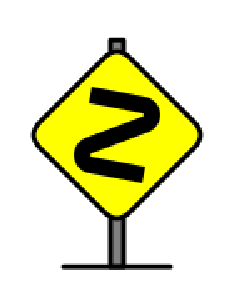
\includegraphics[height=1.3cm]{dbend.eps}
  \end{center}
\end{wrapfigure}
\noindent {\bf Perhatian:} Sebagaimana lazimnya dalam gaya Bourbaki\footnote{Seorang
matematikawan fiktif dan penulis banyak buku matematika bermutu yang tidak
fiktif -- buku-buku itu benar-benar ada -- seperti
\cite{bourbaki2004theory}}, kemunculan simbol ini dalam teks menandai bagian
dengan penalaran yang rumit dan sulit diikuti, atau mengingatkan pembaca pada
kesalahpahaman umum mengenai suatu hal.

\vskip1cm

Versi sumber dalam format PDF tersedia melalui
\href{https://www.poritz.net/jonathan/share/yaintt.pdf}{tautan PDF resmi},
sedangkan seluruh berkas untuk membuat versi khusus tersedia melalui
\href{https://poritz.net/jonathan/share/yaintt/}{direktori sumber resmi}
-- silakan berkreasi; itulah tujuan Creative Commons!
\end{releasenotes}


\ifdefined\suppressToC
  {}
\else
  \tableofcontents
\fi

\mainmatter

\chapter{Keterurutan Baik dan Pembagian}\label{chap:WOaD}

\section{Prinsip Keterurutan Baik dan Induksi Matematika}
\label{sec:WOPaMI}
\begin{discussion}
Dalam bab ini, kita menyajikan tiga alat dasar yang akan sering digunakan untuk
membuktikan sifat-sifat bilangan bulat. Kita mulai dengan sebuah sifat bilangan
  bulat yang sangat penting, yaitu prinsip keterurutan baik. Selanjutnya, kita
  menyatakan apa yang dikenal sebagai prinsip sarang merpati, lalu memperkenalkan
metode penting yang disebut induksi matematika.
\end{discussion}

\subsection{\textbf{Prinsip Keterurutan Baik}}

\begin{definition}\index{elemen terkecil!definisi}
Diberikan suatu himpunan bilangan $S$ (dari jenis apa pun), kita mengatakan
bahwa $\ell\in S$ adalah {\bf elemen terkecil dari $S$} jika
$\forall x\in S$, berlaku $x=\ell$ atau $\ell<x$.
\end{definition}

\begin{WOprinciple}\index{Prinsip Keterurutan Baik!pernyataan}
Setiap himpunan bilangan asli yang tidak kosong memiliki elemen terkecil.
\end{WOprinciple}

\begin{discussion}
Prinsip ini sering diambil sebagai sebuah aksioma.
\end{discussion}

\subsection{\textbf{Prinsip Sarang Merpati}}

\begin{theorem}\index{Prinsip Sarang Merpati!pernyataan}
\label{thm:pigeonhole}
\textbf{Prinsip Sarang Merpati:}
Misalkan $s,k\in\NN$ memenuhi $s>k$. Jika $s$ objek ditempatkan ke dalam $k$
kotak, maka sekurang-kurangnya satu kotak memuat lebih dari satu objek.
\end{theorem}

\begin{proof}
Andaikan setiap kotak memuat paling banyak satu objek. Maka terdapat paling
banyak $k$ objek, padahal terdapat $s$ objek dengan $s>k$.
\end{proof}

\subsection{\textbf{Prinsip Induksi Matematika}}

\begin{discussion}
Sekarang kita menyajikan sebuah alat berharga untuk membuktikan hasil-hasil
mengenai bilangan bulat. Alat ini adalah prinsip induksi matematika.
\end{discussion}

\begin{theorem}
\index{Prinsip Induksi Matematika, versi pertama!pernyataan}
\textbf{Prinsip Pertama Induksi Matematika:}
Misalkan $S\subset\NN$ adalah himpunan yang memenuhi kedua sifat berikut:
\begin{enumerate}
\item $1\in S$; dan
\item $\forall k\in\NN,\ k\in S\Rightarrow k+1\in S$.
\end{enumerate}
Maka $S=\NN$.\newline
Secara lebih umum, misalkan $\Pp(n)$ adalah suatu sifat bilangan asli yang
mungkin benar atau mungkin tidak benar untuk suatu $n\in\NN$ tertentu, dan
memenuhi
\begin{enumerate}
\item $\Pp(1)$ benar; dan
\item $\forall k\in\NN,\ \Pp(k)\Rightarrow\Pp(k+1)$
\end{enumerate}
maka $\forall n\in\NN, \Pp(n)$ benar.
\end{theorem}

\begin{proof}
  Kita menggunakan prinsip keterurutan baik untuk membuktikan prinsip pertama
induksi matematika ini.

Misalkan $S$ adalah himpunan pada bagian pertama teorema dan $T$ adalah himpunan
bilangan asli yang tidak termasuk dalam $S$. Kita akan menggunakan bukti dengan
kontradiksi, jadi andaikan $T$ tidak kosong.

Menurut prinsip keterurutan baik\index{Prinsip Keterurutan Baik!digunakan},
$T$ memiliki elemen terkecil $\ell$.

Perhatikan bahwa $1\in S$, sehingga $1\notin T$ dan akibatnya $\ell>1$. Jadi,
$\ell-1$ adalah bilangan asli. Karena $\ell$ merupakan elemen terkecil dari
$T$, maka $\ell-1$ tidak berada di $T$; oleh karena itu, bilangan tersebut
berada di $S$.

Namun, berdasarkan sifat yang mendefinisikan $S$, karena $\ell-1\in S$, kita
memperoleh $\ell=\ell-1+1\in S$. Hal ini bertentangan dengan fakta bahwa
$\ell$ adalah elemen terkecil dari $T$, sehingga berada di $T$ dan tidak berada
di $S$.

Kontradiksi ini menunjukkan bahwa anggapan bahwa $T$ tidak kosong adalah salah;
dengan demikian, $S=\NN$.

Untuk bagian kedua teorema, ambil
$S=\{n\in\NN\mid\Pp(n)\text{ benar}\}$, lalu terapkan bagian pertama.
\end{proof}

\begin{example}\index{Prinsip Induksi Matematika, versi pertama!digunakan}\label{eg:inductionv1a}
Kita menggunakan induksi matematika untuk menunjukkan bahwa
$\forall n\in \mathbb{N}$,
\begin{equation}
\sum_{j=1}^nj=\frac{n(n+1)}{2}.
\end{equation}
Pertama, perhatikan bahwa
\begin{equation*}
\sum_{j=1}^1j=1=\frac{1\cdot 2}{2}
\end{equation*}
sehingga pernyataan tersebut benar untuk $n=1$. Untuk langkah induksi
selanjutnya, andaikan rumus itu berlaku bagi suatu $n\in\NN$ tertentu, yaitu
$\sum_{j=1}^nj=\frac{n(n+1)}{2}$. Kita tunjukkan bahwa
\begin{equation*}
\sum_{j=1}^{n+1}j=\frac{(n+1)(n+2)}{2}.
\end{equation*}
Dengan demikian, bukti induksi akan lengkap. Memang,
\begin{equation*}
\sum_{j=1}^{n+1}j=\sum_{j=1}^nj+(n+1)=\frac{n(n+1)}{2}+(n+1)=\frac{(n+1)(n+2)}{2},
\end{equation*}
dan hasil yang diinginkan pun diperoleh.
\end{example}

\begin{example}\label{eg:inductionv1b}
Sekarang kita menggunakan induksi matematika untuk membuktikan bahwa
$n!\leq n^n$ untuk setiap $n\in\NN$.
\index{Prinsip Induksi Matematika, versi pertama!digunakan}
\par Perhatikan bahwa $1!=1\leq 1^1=1$. Selanjutnya, kita menyajikan langkah
induksi. Andaikan
\begin{equation*}
n!\leq n^n
\end{equation*}
untuk suatu $n\in\NN$. Kita buktikan bahwa $(n+1)!\leq (n+1)^{n+1}$.
Perhatikan bahwa
\begin{equation*}
(n+1)!=(n+1)n!\leq (n+1)\cdot n^n<(n+1)(n+1)^{n}=(n+1)^{n+1}.
\end{equation*}
Ini melengkapi bukti.
\end{example}

\begin{theorem}
\textbf{Prinsip Kedua Induksi Matematika:}
\index{Prinsip Induksi Matematika, versi kedua!pernyataan}
Misalkan $S\subset\NN$ adalah himpunan yang memenuhi kedua sifat berikut:
\begin{enumerate}
\item $1\in S$; dan
\item $\forall k\in\NN,\ 1,\dots,k\in S\Rightarrow k+1\in S$.
\end{enumerate}
Maka $S=\NN$.\newline
Secara lebih umum, misalkan $\Pp(n)$ adalah suatu sifat bilangan asli yang
mungkin benar atau mungkin tidak benar untuk suatu $n\in\NN$ tertentu, dan
memenuhi
\begin{enumerate}
\item $\Pp(1)$ benar; dan
\item $\forall k\in\NN,$ jika $\Pp(1),\dots,\Pp(k)$ semuanya benar, maka
$\Pp(k+1)$ juga benar,
\end{enumerate}
maka $\forall n\in\NN, \Pp(n)$ benar.
\end{theorem}
\begin{proof}
Untuk membuktikan prinsip kedua induksi, kita menggunakan prinsip pertama
induksi.

Misalkan $S$ adalah himpunan bilangan bulat seperti pada bagian pertama
teorema. Untuk $n\in\NN$, misalkan $\Pp(n)$ adalah sifat matematika
``$1,\dots,n\in S$''. Kita dapat menerapkan Prinsip Pertama Induksi Matematika
untuk membuktikan bahwa $\forall n\in\NN\ \Pp(n)$ benar, yang berarti
$S=\NN$. {\it [Rinciannya diserahkan kepada pembaca.]}

Bagian kedua teorema mengikuti bagian pertama dengan cara yang persis sama
seperti bagian kedua Prinsip Pertama Induksi Matematika mengikuti bagian
pertamanya.
\end{proof}

\ifdefined\suppressallexercises
  {}
\else
  \vfill
  \pagebreak
  \subsection*{Latihan untuk \S\ref{sec:WOPaMI}}
\fi

\begin{exercise}
Buktikan dengan induksi matematika bahwa $n<3^n$ untuk setiap bilangan bulat
positif $n$.
\end{exercise}
\begin{exercise}
Tunjukkan bahwa $\sum_{j=1}^nj^2=\frac{n(n+1)(2n+1)}{6}$.
\end{exercise}
\begin{exercise}
Gunakan induksi matematika untuk membuktikan bahwa\newline
$\sum_{j=1}^n(-1)^{j-1}j^2=(-1)^{n-1}n(n+1)/2$.
\end{exercise}
\begin{exercise}
Gunakan induksi matematika untuk membuktikan bahwa
$\sum_{j=1}^nj^3=[n(n+1)/2]^2$ untuk setiap bilangan bulat positif $n$.
\end{exercise}
\begin{exercise}
Gunakan induksi matematika untuk membuktikan bahwa
$\sum_{j=1}^n(2j-1)=n^2$.
\end{exercise}
\begin{exercise}
Gunakan induksi matematika untuk membuktikan bahwa $2^n<n!$ untuk $n\geq 4$.
\end{exercise}
\begin{exercise}
Gunakan induksi matematika untuk membuktikan bahwa $n^2<n!$ untuk $n\geq 4$.
\end{exercise}

\vfill
\pagebreak

\ifdefined\boundaryone
  \def\finishboundaryone{\backmatter
    \bibliographystyle{amsalpha}
    \bibliography{refs}
    \printindex
    \end{document}}
\else
  \let\finishboundaryone\relax
\fi
\finishboundaryone
\section{Operasi Aljabar pada Bilangan Bulat}\label{sec:AOwI}
Pada $\ZZ$, himpunan bilangan bulat, terdapat dua operasi biner dasar, yaitu
{\bf penjumlahan} (dinotasikan dengan $+$) dan {\bf perkalian} (dinotasikan
dengan $\cdot$). Kedua operasi ini memenuhi sifat-sifat yang sudah dikenal
berikut:

\begin{enumerate}
\item \textbf{Komutativitas penjumlahan dan perkalian}\index{komutativitas penjumlahan dan perkalian}
\begin{align*}
\forall a,b\in\ZZ:\quad a+b&=b+a\\
a\cdot b&=b\cdot a
\end{align*}
\item \textbf{Asosiativitas penjumlahan dan perkalian}\index{asosiativitas penjumlahan dan perkalian}
\begin{align*}
\forall a,b,c\in\ZZ:\quad (a+b)+c&=a+(b+c)\\
(a\cdot b)\cdot c&= a\cdot (b\cdot c)
\end{align*}
\item \textbf{Distributivitas perkalian terhadap penjumlahan}\index{distributivitas perkalian terhadap penjumlahan}
$$
\forall a,b,c\in\ZZ:\quad a\cdot (b+c)=a\cdot b+a\cdot c.\hskip2cm\ 
$$
\end{enumerate}
Di dalam himpunan $\ZZ$ terdapat {\it elemen identitas} untuk kedua operasi
$+$ dan $\cdot$, masing-masing yaitu elemen $0$ dan $1$. Elemen-elemen ini
memenuhi sifat dasar
\begin{align*}
\forall a\in\ZZ:\quad a + 0 &= 0+a = a\\
a\cdot 1 &= 1\cdot a = a\ .
\end{align*}

Setiap elemen dalam himpunan $\ZZ$ mempunyai {\bf invers
aditif}\index{invers aditif}. Artinya, untuk setiap $a\in\ZZ$ terdapat bilangan
bulat lain dalam $\ZZ$, yang dinotasikan dengan $-a$, sedemikian sehingga
\begin{equation}
a+(-a)=0.
\end{equation}
Untuk perkalian, bilangan bulat yang mempunyai {\bf invers
multiplikatif}\index{invers multiplikatif!dalam $\ZZ$} hanyalah $1$ dan $-1$.
Untuk kedua bilangan tersebut, invers multiplikatif yang dinotasikan dengan
$a^{-1}$ atau $1/a$ sama dengan $a$ itu sendiri, sehingga
\begin{equation}
a\cdot a^{-1}=1.
\end{equation}

Dari operasi penjumlahan dan perkalian, kita dapat mendefinisikan dua operasi
lain pada $\ZZ$, yaitu {\bf pengurangan} (dinotasikan dengan $-$) dan {\bf
pembagian} (dinotasikan dengan $/$). Pengurangan merupakan operasi biner pada
$\ZZ$, yakni didefinisikan untuk setiap pasangan bilangan bulat dalam $\ZZ$.
Sebaliknya, pembagian bukan operasi biner pada $\ZZ$ sehingga hanya
didefinisikan untuk pasangan bilangan bulat tertentu. Pengurangan dan
pembagian didefinisikan sebagai berikut:

\begin{enumerate}
\item $\forall a,b\in\ZZ$, $a-b$ didefinisikan sebagai $a+(-b)$.
\item Diberikan $a,b\in\ZZ$ dengan $b\neq 0$. Jika $\exists c\in\ZZ$
sedemikian sehingga $a=b\cdot c$, maka $a/b$ didefinisikan sebagai $c$.
\end{enumerate}

\vfill
\pagebreak
\ifdefined\boundarytwo
  \def\finishboundarytwo{\backmatter
    \bibliographystyle{amsalpha}
    \bibliography{refs}
    \printindex
    \end{document}}
\else
  \let\finishboundarytwo\relax
\fi
\finishboundarytwo
\section{Keterbagian dan Algoritma Pembagian}\label{sec:DaDA}

\begin{discussion}
Sekarang kita membahas konsep keterbagian beserta sifat-sifatnya.
\end{discussion}

\subsection{Keterbagian Bilangan Bulat}
\begin{definition}\index{keterbagian!definisi}
Jika $a$ dan $b$ adalah bilangan bulat dengan $a\neq 0$, kita mengatakan bahwa
{\bf $a$ membagi $b$} dan menulis $a\mid b$ apabila terdapat bilangan bulat $k$
sedemikian sehingga $b=ka$. Dengan kata lain, untuk $a,b\in\ZZ$ dengan
$a\neq 0$, kita menulis $a\mid b$ apabila $\exists k\in\ZZ$ sedemikian sehingga
$b=ka$.

Jika $a$ membagi $b$, kita juga mengatakan bahwa $a$ adalah
{\bf faktor}\index{faktor suatu bilangan bulat} [atau
{\bf pembagi}\index{pembagi}] dari $b$, dan bahwa $b$ adalah
{\bf kelipatan}\index{kelipatan} dari $a$. Jika $a$ tidak membagi $b$, kita
menulis $a\nmid b$.

\end{definition}

\begin{example}
Sebagai contoh, $2\mid 4$ dan $7\mid 63$, sedangkan $5\nmid 26$.
\end{example}

\begin{definition}\index{bilangan bulat genap}\index{bilangan bulat ganjil}
Untuk $a\in\ZZ$, kita mengatakan bahwa $a$ adalah bilangan {\bf genap} jika
$2\mid a$, yaitu jika $\exists k\in\ZZ$ sedemikian sehingga $a=2k$. Sebaliknya,
untuk $a\in\ZZ$, kita mengatakan bahwa $a$ adalah bilangan {\bf ganjil} jika
$2\nmid a$.
\end{definition}

\begin{discussion}
Sebagai konsekuensi dari Algoritma Pembagian\index{Algoritma Pembagian!digunakan}
di bawah ini, jika $a$ ganjil maka $\exists k\in\ZZ$ sedemikian sehingga
$a=2k+1$.
\end{discussion}

\begin{proposition} Untuk setiap $a\in\ZZ\setminus\{0\}$ berlaku $a\mid 0$.
\end{proposition}
\begin{proposition} Jika $a,b\in\ZZ$ memenuhi $|b|<a$ dan $b\neq 0$, maka $a\nmid b$.
\end{proposition}
\begin{proposition} Untuk $a,b\in\ZZ$ dengan $a\neq 0$, berlaku
$a\mid b\Leftrightarrow a\mid|b|$.
\end{proposition}

\begin{theorem}\index{keterbagian!transitivitas}
Jika $a$, $b$, dan $c$ adalah bilangan bulat yang memenuhi $a\mid b$ dan
$b\mid c$, maka $a\mid c$.
\end{theorem}
\begin{proof}
Karena $a\mid b$ dan $b\mid c$, terdapat $k_1,k_2\in\ZZ$ sedemikian sehingga
$b=k_1a$ dan $c=k_2b$. Oleh karena itu, $c=k_1k_2a$, sehingga $a\mid c$.
\end{proof}

\begin{example}\label{eg:divisibility}
Karena $6\mid 18$ dan $18\mid 36$, maka $6\mid 36$.
\end{example}

\begin{discussion}
Teorema berikut menyatakan bahwa jika suatu bilangan bulat membagi dua bilangan
bulat lain, bilangan tersebut juga membagi setiap kombinasi linear keduanya.
\end{discussion}

\begin{theorem}\label{thm:divisibilitylincombs}\index{keterbagian!kombinasi linear}
Untuk setiap $a,b,c,m,n\in\ZZ$, jika $c\mid a$ dan $c\mid b$, maka
$c\mid (ma+nb)$.
\end{theorem}
\begin{proof}
Karena $c\mid a$ dan $c\mid b$, terdapat $k_1,k_2\in\ZZ$ sedemikian sehingga
$a=k_1c$ dan $b=k_2c$. Dengan demikian,
\begin{equation*}
ma+nb=mk_1c+nk_2c=c(mk_1+nk_2),
\end{equation*}
dan karena itu $c\mid (ma+nb)$.
\end{proof}

\begin{discussion}
Teorema~\ref{thm:divisibilitylincombs} dapat diperumum ke setiap kombinasi
linear berhingga sebagai berikut. Jika
\begin{equation*}\index{keterbagian!kombinasi linear}
n\in\NN,\ a,b_1,\dots,b_n\in\ZZ\text{\ dan\ }a\mid b_1, a\mid b_2,\dots,a\mid b_n,
\end{equation*}
maka, untuk setiap $k_1,\dots,k_n\in\ZZ$,
\begin{equation}
a\mid \sum_{j=1}^nk_jb_j
\end{equation}
Pembuktian perumuman ini dengan induksi merupakan latihan yang baik.
\end{discussion}

\subsection{Algoritma Pembagian}

\begin{theorem}\label{thm:theDA}\index{Algoritma Pembagian!pernyataan}
\textbf{Algoritma Pembagian} Diberikan $a,b\in\ZZ$ dengan $b>0$, terdapat
pasangan tunggal $q,r\in\ZZ$ sedemikian sehingga $a=qb+r$ dan $0\leq r<b$.
Bilangan $q$ disebut {\bf hasil bagi}\index{hasil bagi}, sedangkan $r$ disebut
{\bf sisa pembagian $a$ oleh $b$}.\index{sisa pembagian!definisi}
\end{theorem}

\begin{proof}
Perhatikan himpunan $A=\{a-bk\mid k\in\ZZ,\ a-bk\geq 0\}$. Himpunan $A$
tidak kosong karena untuk $k<a/b$ berlaku $a-bk>0$. Menurut prinsip
keterurutan baik\index{Prinsip Keterurutan Baik!digunakan}, $A$ memiliki elemen
terkecil $r=a-qb$ untuk suatu $q\in\ZZ$. Berdasarkan konstruksinya, $r\geq 0$.
Sekarang, jika $r\geq b$, maka (karena $b>0$)
\begin{equation*}
r>r-b=a-qb-b=a-(q+1)b\geq 0.
\end{equation*}
Hal ini menghasilkan kontradiksi karena $r$ diasumsikan sebagai elemen terkecil
$A$. Oleh karena itu, $0\leq r<b$.
\par Selanjutnya kita tunjukkan bahwa $q$ dan $r$ tunggal. Misalkan
$a=q_1b+r_1$ dan $a=q_2b+r_2$, dengan $0\leq r_1<b$ dan $0\leq r_2<b$. Maka
\begin{equation*}
a-a=q_1b+r_1-(q_2b+r_2)=(q_1-q_2)b+(r_1-r_2)=0.
\end{equation*}
Akibatnya,
\begin{equation*}
(q_1-q_2)b=r_2-r_1.
\end{equation*}
Jadi,
\begin{equation*}
b\mid (r_2-r_1).
\end{equation*}
Karena $0\leq|r_2-r_1|\leq\max(r_1,r_2)$ dan $b>\max(r_1,r_2)$, maka
$r_2-r_1$ harus sama dengan $0$, yaitu $r_2=r_1$. Karena
$bq_1+r_1=bq_2+r_2$, kita juga memperoleh $q_1=q_2$. Hal ini membuktikan
ketunggalan.
\end{proof}

\begin{example}\label{eg:arithmetic}
Jika $a=71$ dan $b=6$, maka $71=6\cdot 11+5$. Di sini $q=11$ dan $r=5$.
\end{example}

\ifdefined\suppressallexercises
  {}
\else
  \vfill
  \pagebreak
  \subsection*{Latihan untuk \S\ref{sec:DaDA}}
\fi

\begin{exercise}
Tunjukkan bahwa $5\mid 25$, $19\mid38$, dan $2\mid 98$.
\end{exercise}
\begin{exercise}
Gunakan Algoritma Pembagian untuk menentukan hasil bagi dan sisa ketika 76
dibagi oleh 13.
\end{exercise}
\begin{exercise}
Gunakan Algoritma Pembagian untuk menentukan hasil bagi dan sisa ketika -100
dibagi oleh 13.
\end{exercise}
\begin{exercise}
Tunjukkan bahwa jika $a,b,c$, dan $d$ adalah bilangan bulat, dengan $a$ dan $c$
tidak nol, serta $a\mid b$ dan $c\mid d$, maka $ac\mid bd$.
\end{exercise}
\begin{exercise}\label{exer:sizeofdivisors}
Tunjukkan bahwa jika $a$ dan $b$ adalah bilangan bulat positif dan $a\mid b$,
maka $a\leq b$.
\end{exercise}
\begin{exercise}
Buktikan bahwa jumlah dua bilangan bulat genap adalah genap, jumlah dua bilangan
bulat ganjil adalah genap, dan jumlah sebuah bilangan bulat genap dengan sebuah
bilangan bulat ganjil adalah ganjil.
\end{exercise}
\begin{exercise}
Tunjukkan bahwa hasil kali dua bilangan bulat genap adalah genap, hasil kali dua
bilangan bulat ganjil adalah ganjil, dan hasil kali sebuah bilangan bulat genap
dengan sebuah bilangan bulat ganjil adalah genap.
\end{exercise}
\begin{exercise}
Tunjukkan bahwa jika $m$ adalah bilangan bulat, maka $3$ membagi $m^3-m$.
\end{exercise}
\begin{exercise}
Tunjukkan bahwa kuadrat setiap bilangan bulat ganjil berbentuk $8m+1$ untuk
suatu $m\in\ZZ$.
\end{exercise}
\begin{exercise}
Tunjukkan bahwa untuk setiap bilangan bulat $n$, kuadrat $n$ berbentuk $3m$
atau $3m+1$ untuk suatu $m\in\ZZ$, tetapi tidak pernah berbentuk $3m+2$ untuk
$m\in\ZZ$.
\end{exercise}
\begin{exercise}
Tunjukkan bahwa jika $ac\mid bc$, maka $a\mid b$.
\end{exercise}
\begin{exercise}
Tunjukkan bahwa jika $a\mid b$ dan $b\mid a$, maka $a=\pm b$.
\end{exercise}

\vfill
\pagebreak
\ifdefined\boundarythree
  \def\finishboundarythree{\backmatter
    \bibliographystyle{amsalpha}
    \bibliography{refs}
    \printindex
    \end{document}}
\else
  \let\finishboundarythree\relax
\fi
\finishboundarythree
\section{Representasi Bilangan Bulat dalam Berbagai Basis}\label{sec:RoIiDB}
\begin{discussion}
Pada bagian ini, kita menunjukkan bahwa setiap bilangan bulat positif dapat
dituliskan secara unik dalam ekspansi pada sebarang basis bilangan bulat yang
lebih besar dari $1$. Biasanya kita menggunakan notasi desimal untuk
merepresentasikan bilangan bulat. Kita akan menunjukkan cara mengubah bilangan
bulat dari notasi desimal ke notasi dengan sebarang basis bilangan bulat lain,
dan sebaliknya. Notasi desimal mungkin menjadi tradisi dalam kehidupan
sehari-hari semata-mata karena kita memiliki sepuluh jari tangan. (``Lalu
bagaimana dengan jari kaki kita?'' protes Anda. Saya tidak tahu. Dan tampaknya
bangsa Babilonia memiliki $30$ jari pada setiap tangan, atau $15$ jari pada
setiap tangan dan kaki, sebab mereka menggunakan basis $60$.)
\end{discussion}

\textbf{Notasi} Bilangan bulat $a$ yang ditulis dalam ekspansi basis $b$
dilambangkan dengan $(a)_b$.

\begin{theorem}\label{thm:basebexpansion}
Misalkan $b\in\ZZ$ memenuhi $b>1$. Maka, untuk setiap $m\in\NN$, terdapat
tepat satu $l\in\ZZ_{\geq 0}$ beserta digit-digit $a_0,a_1,\dots,a_l\in\ZZ$
sedemikian sehingga
\begin{align*}
m=\sum_{j=0}^{l}a_jb^j,\\
0\leq a_j<b\text{\ untuk\ }j=0,1,\dots,l,\text{\ dan}\ \ \ \\
a_l\neq 0.\hskip2.5cm
\end{align*}
\end{theorem}
\begin{proof}
Ambil sebarang $m\in\NN$. Mula-mula kita membagi $m$ dengan
$b$ menggunakan Algoritma Pembagian\index{Algoritma Pembagian!digunakan},
sehingga diperoleh
\begin{equation*}
m=q_0b+a_0, \ \ \ 0\leq a_0 <b.
\end{equation*}
Jika $q_0\neq 0$, selanjutnya kita membagi $q_0$ dengan $b$ dan memperoleh
\begin{equation*}
q_0=q_1b+a_1, \ \ \ 0\leq a_1<b.
\end{equation*}
Jika $q_0=0$, ambil $l=0$ dan $a_0=m$; bagian eksistensi selesai. Selanjutnya,
anggap $q_0>0$. Karena setiap hasil bagi positif berikutnya lebih kecil daripada
hasil bagi sebelumnya, untuk suatu $l\geq1$ proses ini pertama kali berakhir
pada $q_l=0$. Dengan demikian,
\begin{align*}
q_{j-1}&=q_jb+a_j, \qquad 0\leq a_j<b \quad (j=1,\dots,l),\\
q_l&=0, \qquad a_l=q_{l-1}\neq0.
\end{align*}
\par Sekarang, dengan menyubstitusikan persamaan $q_0=q_1b+a_1$ ke dalam
$m=q_0b+a_0$, diperoleh
\begin{equation*}
m=(q_1b+a_1)b+a_0=q_1b^2+a_1b+a_0.
\end{equation*}
Dengan menyubstitusikan persamaan-persamaan tersebut secara berturut-turut
(atau dengan induksi pada $j$), diperoleh
\begin{align*}
m&=q_{j-1}b^j+\sum_{i=0}^{j-1}a_ib^i \qquad (j=1,\dots,l),\\
 &=a_lb^l+\sum_{i=0}^{l-1}a_ib^i
 =\sum_{i=0}^{l}a_ib^i.
\end{align*}
Yang masih harus dibuktikan ialah bahwa representasi tersebut tunggal. Sekarang
misalkan
\begin{equation*}
m=\sum_{i=0}^{l}a_ib^i=\sum_{i=0}^{s}c_ib^i.
\end{equation*}
Ambil $L=\max\{l,s\}$ dan tambahkan koefisien nol pada ekspansi yang lebih
pendek. Dengan mengurangkan kedua ekspansi tersebut, diperoleh
\begin{equation*}
\sum_{i=0}^{L}(a_i-c_i)b^i=0.
\end{equation*}
Jika kedua ekspansi berbeda, ambil indeks terkecil $0\leq j\leq L$ sedemikian
sehingga $c_j\neq a_j$. Semua suku berindeks lebih kecil daripada $j$ lenyap,
sehingga diperoleh
\begin{equation*}
b^j\sum_{i=j}^{L}(a_i-c_i)b^{i-j}=0,
\end{equation*}
dan karena $b\neq 0$, diperoleh
\begin{equation*}
\sum_{i=j}^{L}(a_i-c_i)b^{i-j}=0.
\end{equation*}
Oleh karena itu,
\begin{equation*}
a_j-c_j=-b\sum_{i=j+1}^{L}(a_i-c_i)b^{i-j-1},
\end{equation*}
sehingga $b\mid (a_j-c_j)$. Karena $0\leq a_j<b$ dan $0\leq c_j<b$,
berlaku $|a_j-c_j|<b$. Dengan demikian, $a_j=c_j$. Ini bertentangan dengan
pemilihan $j$, sehingga ekspansi tersebut tunggal.
\end{proof}

\begin{definition}\label{def:baseb}\index{basis $b$}
Misalkan $b\in\ZZ$ memenuhi $b>1$. Untuk $m\in\NN$, misalkan
$\ell\in\ZZ_{\geq 0}$ dan $a_0,a_1,\dots,a_\ell\in\ZZ$ sebagaimana dalam teorema di
atas (\ref{thm:basebexpansion}). Maka {\bf representasi basis $b$ dari $m$}
adalah rangkaian digit $(m)_b=a_\ell\dots a_1a_0$. Jika $b\ge10$, kita sering
menggunakan simbol tunggal lain untuk merepresentasikan nilai-nilai $a_i$ yang
mungkin, dari $10$ sampai $b-1$. Sebagai contoh,
\begin{align*}
10&\leftrightsquigarrow A\\
11&\leftrightsquigarrow B\\
12&\leftrightsquigarrow C\\
&\text{\it dst.}
\end{align*}
Representasi bilangan bulat dalam basis 2 disebut
{\bf representasi biner}\index{representasi biner}. Representasi biner berguna
bagi komputer: semua koefisien $a_0,\dots,a_\ell$ dalam representasi biner
memenuhi $0\leq a_j<2$, sehingga nilainya 0 atau 1. Jadi, untuk
merepresentasikan bilangan bulat melalui $\ell+1$ kawat, setiap kawat dapat
diberi tegangan (1) atau tidak (0). (Istilah {\it bit}\index{bit} berasal dari
frasa bahasa Inggris {\it binary digit}, yang berarti ``digit biner''.)

Pemrogram komputer juga sering menggunakan basis 8 dan basis 16, yang
masing-masing disebut {\bf oktal}\index{oktal} dan
{\bf heksadesimal}\index{heksadesimal}, atau
{\bf heks}\index{heks}. Bangsa Babilonia menggunakan basis $60$, yang disebut
{\bf seksagesimal}\index{seksagesimal}.
\end{definition}

\begin{example}\label{eg:basetwo}
Untuk mencari ekspansi basis 3 dari 214, kita melakukan pembagian berikut:
\begin{align*}
214&=3\cdot 71+1\\
71&= 3\cdot 23+2\\
23&= 3\cdot 7+2\\
7&= 3\cdot 2+1\\
2&= 3\cdot 0+2\\
\end{align*}
Untuk memperoleh ekspansi basis 3 dari 214, kita membaca sisa-sisa pembagian
tersebut dari bawah ke atas, sehingga $(214)_{10}=(21221)_3$.
\end{example}

\begin{example}\label{eg:changebase}
Untuk mencari ekspansi basis $10$, yaitu ekspansi desimal, dari $(364)_7$, kita
menghitung $4\cdot 7^0+6\cdot 7^1+3\cdot 7^2=4+42+147=193$.
\end{example}

\ifdefined\suppressallexercises
  {}
\else
  \vfill
  \pagebreak
  \subsection{Latihan untuk \S\ref{sec:RoIiDB}}
\fi

\begin{exercise}
Ubah $(7482)_{10}$ ke notasi basis 6.
\end{exercise}
\begin{exercise}
Ubah $(98156)_{10}$ ke notasi basis 8.
\end{exercise}
\begin{exercise}
Ubah $(101011101)_2$ ke notasi desimal.
\end{exercise}
\begin{exercise}
Ubah $(AB6C7D)_{16}$ ke notasi desimal.
\end{exercise}
\begin{exercise}
Ubah $(9A0B)_{16}$ ke notasi biner.
\end{exercise}

\vfill
\pagebreak
\ifdefined\boundaryfour
  \def\finishboundaryfour{\backmatter
    \bibliographystyle{amsalpha}
    \bibliography{refs}
    \printindex
    \end{document}}
\else
  \let\finishboundaryfour\relax
\fi
\finishboundaryfour
\section{Faktor Persekutuan Terbesar}\label{gcd}
\begin{discussion}
Pada bagian ini kita mendefinisikan faktor persekutuan terbesar (FPB) dari dua
bilangan bulat dan membahas sifat-sifatnya. Kita juga membuktikan bahwa FPB dua
bilangan bulat merupakan kombinasi linear dari kedua bilangan tersebut.

Jika dua bilangan bulat $a$ dan $b$ tidak keduanya $0$, setidaknya salah
satunya taknol dan hanya mempunyai berhingga banyak pembagi (lihat
Latihan~\ref{exer:sizeofdivisors}). Karena itu, $a$ dan $b$ hanya mempunyai
berhingga banyak pembagi bersama. Pada bagian ini kita membahas pembagi terbesar
di antara pembagi-pembagi bersama tersebut.
\end{discussion}

\begin{definition}\index{faktor persekutuan terbesar!definisi}
Untuk $a,b\in\ZZ$ yang tidak keduanya nol, {\bf faktor persekutuan
terbesar} adalah bilangan bulat terbesar yang membagi $a$ sekaligus $b$, dan
ditulis $\gcd(a,b)$ (atau kadang-kadang cukup $(a,b)$).

Jika hal ini menyederhanakan suatu rumus, kita menetapkan $\gcd(0,0)=0$.
\end{definition}

\begin{example}\label{eg:gcda}\index{faktor persekutuan terbesar!contoh}
Faktor persekutuan terbesar dari 24 dan 18 adalah 6. Dengan kata lain,
$\gcd(24,18)=6$.
\end{example}

\begin{definition}\index{relatif prima!definisi}
Bilangan $a,b\in\ZZ$ disebut {\bf relatif prima} jika $\gcd(a,b)=1$.
\index{faktor persekutuan terbesar!digunakan}
\end{definition}

\begin{example}\label{eg:gcdb}
Faktor persekutuan terbesar dari 9 dan 16 adalah 1; jadi, kedua bilangan
tersebut relatif prima.
\end{example}

\begin{discussion}
Perhatikan bahwa setiap bilangan bulat mempunyai pembagi positif dan negatif.
Jika $a$ adalah pembagi positif dari $m$, maka $-a$ juga merupakan pembagi dari
$m$. Karena itu, dari definisi faktor persekutuan terbesar terlihat bahwa
$\gcd(a,b)=\gcd(|a|, |b|)$.
\index{faktor persekutuan terbesar!sifat}

Kita dapat menggunakan FPB dua bilangan bulat untuk membentuk bilangan-bilangan
yang relatif prima:
\end{discussion}
\begin{theorem}\label{thm:dividebygcd}\index{relatif prima}
Jika $a,b\in\ZZ$ tidak keduanya nol dan $\gcd(a,b)=d$, maka
\\
$\gcd(a/d,b/d)=1$.
\index{faktor persekutuan terbesar!digunakan}
\end{theorem}
\begin{proof}
Ambil $a,b\in\ZZ$. Kita akan menunjukkan bahwa $a/d$ dan $b/d$ tidak
mempunyai pembagi bersama positif selain $1$. Misalkan $k\in\NN$ membagi
$a/d$ sekaligus $b/d$. Maka $\exists m,n\in\ZZ$ sedemikian sehingga
\begin{equation*}
a/d=km \hspace{0.3 cm}\mbox{dan} \ \  b/d=kn
\end{equation*}
Dengan demikian,
\begin{equation*}
a=kmd \hspace{0.3 cm}\mbox{dan} \ \  b=knd.
\end{equation*}
Jadi, $kd$ merupakan pembagi bersama dari $a$ dan $b$. Selain itu,
$kd\geq d$. Namun, $d$ adalah faktor persekutuan terbesar dari $a$ dan $b$,
sehingga $kd\leq d$. Oleh karena itu, $k=1$.
\end{proof}

\begin{discussion}
Teorema berikut menunjukkan bahwa faktor persekutuan terbesar dari dua bilangan
bulat tidak berubah ketika suatu kelipatan dari salah satunya ditambahkan pada
bilangan yang lain.
\end{discussion}

\begin{theorem}\index{faktor persekutuan terbesar!sifat}
Misalkan $a,b,c\in\ZZ$. Maka $\gcd(a,b)=\gcd(a+cb,b)$.
\end{theorem}

\begin{proof}
Kita akan menunjukkan bahwa setiap pembagi bersama dari $a$ dan $b$ juga
merupakan pembagi bersama dari $a+cb$ dan $b$, demikian pula sebaliknya. Jadi,
kedua pasangan itu mempunyai himpunan pembagi bersama yang persis sama. Karena
itu, faktor persekutuan terbesar dari $a$ dan $b$ juga menjadi faktor
persekutuan terbesar dari $a+cb$ dan $b$. Misalkan $k$ adalah pembagi bersama
dari $a$ dan $b$. Menurut Teorema~\ref{thm:divisibilitylincombs},
$k \mid (a+cb)$, sehingga $k$ membagi $a+cb$. Sekarang misalkan $l$ adalah
pembagi bersama dari $a+cb$ dan $b$. Sekali lagi, menurut
Teorema~\ref{thm:divisibilitylincombs},
\begin{equation*}
l\mid ((a+cb)-cb)=a.
\end{equation*}
Jadi, $l$ merupakan pembagi bersama dari $a$ dan $b$, dan hasil yang dimaksud
pun terbukti.
\end{proof}

\begin{example}\label{eg:gcdc}\index{faktor persekutuan terbesar!contoh}
Perhatikan bahwa $\gcd(4,14)=\gcd(4,14-3\cdot 4)=\gcd(4,2)=2$.
\end{example}

\begin{discussion}
Sekarang kita menyajikan teorema yang membuktikan bahwa faktor persekutuan
terbesar dari dua bilangan bulat dapat ditulis sebagai kombinasi linear dari
kedua bilangan tersebut.
\end{discussion}

\begin{theorem}\label{thm:gcdislincomb}
\index{faktor persekutuan terbesar!sifat}
Misalkan $a,b\in\ZZ$ tidak keduanya nol. Maka $\gcd(a,b)$ adalah bilangan
asli terkecil yang berbentuk $d=ma+nb$ untuk suatu $m,n\in\ZZ$.
\end{theorem}

\begin{proof}
Dengan mengganti $a$ dan $b$ masing-masing oleh $|a|$ dan $|b|$ serta menyerap
tandanya ke dalam koefisien, tanpa mengurangi keumuman kita dapat menganggap
$a,b\geq 0$ dan tidak keduanya nol. Tinjau himpunan
\begin{equation*}
S=\{d\in\NN\mid d=ma+nb\text{\ untuk suatu\ }m,n\in\ZZ\}\ .
\end{equation*}
$S$ tidak kosong karena setidaknya salah satu dari $a$ dan $b$ positif. Jika
$a>0$, maka $a=1\cdot a+0\cdot b\in S$; jika $b>0$, maka
$b=0\cdot a+1\cdot b\in S$. Misalkan $d\in\NN$ adalah elemen terkecil
dari $S$; keberadaannya dijamin oleh Prinsip Keterurutan Baik. Karena $d\in S$,
terdapat $m,n\in\ZZ$ sedemikian sehingga $d=ma+nb$. Kita masih harus
membuktikan bahwa $d$ membagi $a$ sekaligus $b$ dan bahwa $d$ adalah pembagi
bersama terbesar dengan sifat tersebut.

Menurut Algoritma Pembagian, $\exists q,r\in\ZZ$ sedemikian sehingga
\begin{equation*}
a=qd+r, \ \ \ 0\leq r<d.
\end{equation*}
Dengan demikian,
\begin{equation*}
r=a-qd=a-q(ma+nb)=(1-qm)a-qnb.
\end{equation*}
Jadi, $r$ merupakan kombinasi linear dari $a$ dan $b$. Karena $0\leq r<d$
dan $d$ adalah bilangan bulat positif terkecil yang merupakan kombinasi linear
dari $a$ dan $b$, haruslah $r=0$, sehingga $a=qd$. Jadi, $d\mid a$.

Argumen yang sama menunjukkan bahwa $d\mid b$.

Sekarang, misalkan $c$ membagi $a$ sekaligus $b$. Menurut
Teorema~\ref{thm:divisibilitylincombs}, $c$ membagi setiap kombinasi linear
dari $a$ dan $b$. Jadi, $c\mid d$. Hal ini membuktikan bahwa setiap pembagi
bersama dari $a$ dan $b$ membagi $d$. Karena itu, $c\leq d$, dan $d$ adalah
faktor persekutuan terbesar.
\end{proof}

\begin{discussion}
Berikut suatu penerapan sederhana yang akan sangat berguna kelak:
\end{discussion}
\begin{corollary}\label{cor:intlincombrelprime}\index{relatif prima!kombinasi linear yang menghasilkan $1$}
Jika $a,b\in\ZZ$ relatif prima, maka $\exists m,n\in\ZZ$ sedemikian sehingga
$ma+nb=1$.
\end{corollary}

\begin{definition}\index{faktor persekutuan terbesar!definisi untuk lebih dari dua bilangan bulat}
Untuk suatu $n\in\NN$, misalkan $a_1,a_2,\dots,a_n\in\ZZ$ tidak semuanya
$0$. {\bf Faktor persekutuan terbesar} dari bilangan-bilangan tersebut adalah
bilangan bulat terbesar yang membagi semuanya, dan dilambangkan dengan
$\gcd(a_1,\dots,a_n)$.
\end{definition}
\begin{definition}\index{relatif prima secara bersama-sama}
Untuk suatu $n\in\NN$, bilangan-bilangan $a_1,a_2,\dots,a_n\in\ZZ$
disebut {\bf relatif prima secara bersama-sama} jika
$\gcd(a_1,a_2,\dots,a_n)=1$.
\index{faktor persekutuan terbesar!digunakan}
\end{definition}

\begin{example}\label{eg:mutrelprime}
Bilangan-bilangan bulat $3, 6, 7$ relatif prima secara bersama-sama karena
$(3,6,7)=1$, meskipun $(3,6)=3$.
\end{example}

\begin{definition}\index{relatif prima berpasangan!definisi}
Untuk suatu $n\in\NN$, bilangan-bilangan $a_1,a_2,\dots,a_n\in\ZZ$
disebut {\bf relatif prima berpasangan} jika $\forall i,j\in\NN$ dengan
$i\le n$, $j\le n$, dan $i\neq j$, berlaku $\gcd(a_i,a_j)=1$.
\index{faktor persekutuan terbesar!digunakan}
\end{definition}

\begin{example}\label{eg:pairwiserelprime}
Bilangan-bilangan bulat $3,14,25$ relatif prima berpasangan. Perhatikan pula
bahwa bilangan-bilangan tersebut relatif prima secara bersama-sama.
\end{example}

\begin{proposition}
Untuk $n\in\NN$ dengan $n\geq 2$ dan $a_1,\dots,a_n\in\ZZ$, jika
$a_1,a_2,\dots,a_n$ relatif prima berpasangan, maka bilangan-bilangan tersebut
relatif prima secara bersama-sama.
\end{proposition}

\ifdefined\suppressallexercises
  {}
\else
  \vfill
  \pagebreak
  \subsection*{Latihan untuk \S\ref{gcd}}
\fi

\begin{exercise}
Tentukan faktor persekutuan terbesar dari 15 dan 35.
\index{faktor persekutuan terbesar!contoh}
\end{exercise}
\begin{exercise}
Tentukan faktor persekutuan terbesar dari 100 dan 104.
\index{faktor persekutuan terbesar!contoh}
\end{exercise}
\begin{exercise}
Tentukan faktor persekutuan terbesar dari -30 dan 95.
\index{faktor persekutuan terbesar!contoh}
\end{exercise}
\begin{exercise}
Misalkan $m\in\NN$. Tentukan faktor persekutuan terbesar dari $m$ dan
$m+1$.
\index{faktor persekutuan terbesar!contoh}
\end{exercise}
\begin{exercise}
Misalkan $m\in\NN$. Tentukan faktor persekutuan terbesar dari $m$ dan
$m+2$.
\index{faktor persekutuan terbesar!contoh}
\end{exercise}
\begin{exercise}
Tunjukkan bahwa jika $m,n\in\ZZ$ memenuhi $\gcd(m,n)=1$, maka
$\gcd(m+n,m-n)=1$ atau $2$.
\index{faktor persekutuan terbesar!sifat}
\end{exercise}
\begin{exercise}
Tunjukkan bahwa jika $m\in\NN$, maka $3m+2$ dan $5m+3$ relatif prima.
\index{faktor persekutuan terbesar!sifat}
\end{exercise}
\begin{exercise}
Tunjukkan bahwa jika $a,b\in\ZZ$ relatif prima, maka
$\gcd(a+2b,2a+b)=1$ atau $3$.
\index{faktor persekutuan terbesar!sifat}
\end{exercise}
\begin{exercise}
Tunjukkan bahwa jika $a_1,a_2,\dots,a_n\in\ZZ$ tidak semuanya $0$ dan
$c\in\NN$, maka
\index{faktor persekutuan terbesar!sifat}
$\gcd(ca_1,ca_2,\dots,ca_n)=c\cdot\gcd(a_1,a_2,\dots,a_n).$
\end{exercise}

\vfill
\pagebreak
\ifdefined\boundaryfive
  \def\finishboundaryfive{\backmatter
    \bibliographystyle{amsalpha}
    \bibliography{refs}
    \printindex
    \end{document}}
\else
  \let\finishboundaryfive\relax
\fi
\finishboundaryfive
\section{Algoritma Euklides}\label{sec:EA}
\begin{discussion}
Pada bagian ini kita menjelaskan metode sistematis untuk menentukan faktor
persekutuan terbesar dari dua bilangan bulat. Metode ini berasal dari Euklides
dan karena itu disebut Algoritma Euklides.
\end{discussion}
\begin{lemma}\label{lem:gcdafterdivision}\index{faktor persekutuan terbesar!setelah algoritma pembagian}
Jika $a,b,q,r\in\ZZ$ dan $a=qb+r$, maka $\gcd(a,b)=\gcd(r,b)$.
\end{lemma}
\begin{proof}
Menurut sifat invariansi FPB terhadap penambahan kelipatan yang dibuktikan pada
bagian sebelumnya, $\gcd(bq+r,b)=\gcd(b,r)$.
\end{proof}

\begin{discussion}
Sekarang kita beralih ke bentuk umum Algoritma Euklides. Pada dasarnya,
algoritma ini menyatakan bahwa faktor persekutuan terbesar dari dua bilangan
bulat adalah sisa taknol terakhir dalam pembagian berulang.
\end{discussion}

\begin{theorem}\index{Algoritma Euklides!pernyataan}
\label{thm:euclideanalg}
Misalkan $a,b\in\NN$ dan $a\geq b$. Tetapkan $r_0=a$, $r_1=b$, $s_0=1$,
$s_1=0$, $t_0=0$, dan $t_1=1$. Terapkan Algoritma Pembagian secara berulang:
selama $r_{j+1}\neq 0$, tentukan $q_{j+1}\in\NN$ dan
$r_{j+2}\in\ZZ_{\geq 0}$ sedemikian sehingga
$r_j=r_{j+1}q_{j+1}+r_{j+2}$ dan $0\leq r_{j+2}<r_{j+1}$. Berhentilah pada
indeks $n$ yang memenuhi $r_n>0$ dan $r_{n+1}=0$. Pada setiap langkah, tetapkan
$s_{j+2}=s_j-q_{j+1}s_{j+1}$ dan
$t_{j+2}=t_j-q_{j+1}t_{j+1}$. Maka
$\gcd(a,b)=r_n=s_na+t_nb$.
\end{theorem}
\begin{proof}
Dengan menerapkan Algoritma Pembagian, diperoleh
\begin{align*}
r_j&=q_{j+1}r_{j+1}+r_{j+2},
    &&0\leq r_{j+2}<r_{j+1}\quad (j=0,1,\dots,n-1).
\end{align*}
Proses ini akhirnya menghasilkan sisa $0$, sebab selama sisanya taknol,
sisa-sisa tersebut membentuk barisan menurun ketat dari bilangan bulat
taknegatif. Menurut Lema~\ref{lem:gcdafterdivision},
\begin{equation*}
\gcd(a,b)=\gcd(r_0,r_1)=\gcd(r_n,r_{n+1})=\gcd(r_n,0)=r_n.
\end{equation*}
\end{proof}
\noindent{\bf Catatan:} Versi lengkap teorema ini, yang menyertakan $s_j$ dan
$t_j$, disebut {\bf Algoritma Euklides diperluas}, sedangkan versi yang lebih
sederhana tanpa koefisien-koefisien tersebut disebut {\bf Algoritma Euklides}.

\begin{discussion}
Pembaca yang teliti akan melihat bahwa kita belum membuktikan klaim bahwa
$s_j$ dan $t_j$ dapat digunakan untuk menuliskan FPB sebagai kombinasi linear
dari $a$ dan $b$. Bukti tersebut diserahkan sebagai latihan di bawah ini.
\end{discussion}

\begin{example}\label{eg:EA}
Kita akan menentukan faktor persekutuan terbesar dari $4147$ dan $10672$.
Perhatikan bahwa
\begin{align*}
10672&=4147\cdot 2+2378,\\
 4147&=2378\cdot 1+1769,\\
 2378&=1769\cdot 1+609,\\
 1769&=609\cdot 2 +551,\\
  609&=551\cdot 1+58, \\
  551&=58\cdot 9+ 29,\\
   58&=29\cdot 2,\\
\end{align*}
Jadi, $\gcd(4147,10672)=29$.\index{faktor persekutuan terbesar!contoh}
\end{example}

\ifdefined\suppressallexercises
  {}
\else
  \vfill
  \pagebreak
  \subsection*{Latihan untuk \S\ref{sec:EA}}
\fi

\begin{exercise}
Gunakan Algoritma Euklides untuk menentukan faktor persekutuan terbesar dari
412 dan 32, lalu nyatakan hasilnya sebagai kombinasi linear kedua bilangan
tersebut.
\index{faktor persekutuan terbesar!contoh}
\end{exercise}
\begin{exercise}
Gunakan Algoritma Euklides untuk menentukan faktor persekutuan terbesar dari
780 dan 150, lalu nyatakan hasilnya sebagai kombinasi linear kedua bilangan
tersebut.
\index{faktor persekutuan terbesar!contoh}
\end{exercise}
\begin{exercise}
Tentukan faktor persekutuan terbesar dari $70,98,108$.
\index{faktor persekutuan terbesar!contoh}
\end{exercise}
\begin{exercise}
Misalkan $a,b\in\NN$ genap. Buktikan bahwa
$\gcd(a,b)=2\gcd(a/2,b/2)$.
\index{faktor persekutuan terbesar!sifat}
\end{exercise}
\begin{exercise}
Tunjukkan bahwa jika $a\in\NN$ genap dan $b\in\NN$ ganjil, maka
$\gcd(a,b)=\gcd(a/2,b)$.\index{faktor persekutuan terbesar!sifat}
\end{exercise}
\begin{exercise}
Buktikan klaim mengenai koefisien dalam Algoritma Euklides diperluas.
\end{exercise}

\ifdefined\boundarysix
  \def\finishboundarysix{\backmatter
    \bibliographystyle{amsalpha}
    \bibliography{refs}
    \printindex
    \end{document}}
\else
  \let\finishboundarysix\relax
\fi
\finishboundarysix

\chapter{Kongruensi}\label{chap:Cs}

\begin{discussion}
Kongruensi tidak lebih dari sebuah pernyataan mengenai keterbagian. Teori
kongruensi diperkenalkan oleh Carl Friedrich
Gauss,\index{Gauss, Carl Friedrich} dalam karya monumentalnya
{\it Disquisitiones Arithmeticae} (diterbitkan pada tahun 1801, ketika ia
berusia 24 tahun; terjemahannya terdapat dalam
\cite{gauss1986disquisitiones}).
\index{Disquisitiones Arithmeticae}

Kita mulai dengan memperkenalkan kongruensi beserta sifat-sifatnya.
Kemudian kita menyajikan solusi kongruensi linear sebagai pengantar menuju
Teorema Sisa Cina yang akan dibahas sesudahnya.
\end{discussion}

\section{Pengantar Kongruensi}\label{sec:ItC}
\begin{discussion}
Seperti disebutkan dalam pengantar, teori kongruensi dikembangkan oleh Gauss
pada awal abad kesembilan belas.
\end{discussion}
\begin{definition}\index{kongruen!definisi}
Untuk $a,b\in\ZZ$ dan $n\in\NN$, kita mengatakan bahwa {\bf $a$
kongruen dengan $b$ modulo $n$} jika $n \mid (a-b)$, yakni jika
$\exists k\in\ZZ$ sedemikian sehingga $a=b+kn$. Jika $a$ kongruen dengan
$b$ modulo $n$, kita menulis $a\equiv b\pmod{n}$.
\end{definition}

\begin{example}\label{eg:congruences}
$19\equiv 5\pmod7$. Demikian pula, $2k+1 \equiv 1\pmod2$, yang berarti
bahwa setiap bilangan ganjil kongruen dengan 1 modulo 2.
\end{example}

\begin{discussion}
Dalam banyak hal, kongruensi sangat menyerupai kesamaan. Sebagai contoh:
\end{discussion}

\begin{theorem}\label{thm:basiccongprops}\index{kongruen!sifat dasar}
Misalkan $a,b,c,d\in\ZZ$ dan $n\in\NN$. Maka

\begin{enumerate}
\item Jika $a\equiv b\pmod n$, maka $b\equiv a\pmod n$.
\item Jika $a\equiv b\pmod n$ dan $b\equiv c\pmod n$, maka
$a\equiv c\pmod n$.
\item Jika $a\equiv b\pmod n$, maka $a+c \equiv b+c\pmod n$.
\item Jika $a\equiv b\pmod n$, maka $a-c \equiv b-c\pmod n$.
\item Jika $a\equiv b\pmod n$, maka $ac \equiv bc\pmod n$.
\item Jika $c>0$ dan $a\equiv b\pmod n$, maka $ac \equiv bc\pmod{nc}$.
\item Jika $a\equiv b\pmod n$ dan $c \equiv d\pmod n$, maka
$a+c \equiv b+d\pmod n$.
\item Jika $a\equiv b\pmod n$ dan $c \equiv d\pmod n$, maka
$a-c \equiv b-d\pmod n$.
\item Jika $a\equiv b\pmod n$ dan $c \equiv d\pmod n$, maka
$ac \equiv bd\pmod n$.
\end{enumerate}
\end{theorem}
\begin{proof}\ 
\begin{enumerate}
\item Jika $a \equiv b\pmod n$, maka $n\mid (a-b)$. Jadi terdapat
$k\in\ZZ$ sedemikian sehingga $a-b=kn$. Hal ini mengakibatkan
$b-a=(-k)n$, sehingga $n\mid (b-a)$. Dengan demikian,
$b\equiv a\pmod n$.
\item Karena $a\equiv b\pmod n$ dan $b\equiv c\pmod n$, berlaku
$n\mid (a-b)$ dan $n\mid (b-c)$. Oleh karena itu, terdapat $k,l\in\ZZ$
sedemikian sehingga $a=b+kn$ dan $b=c+ln$. Akibatnya,
$a=c+(k+l)n$. Dengan kata lain, $a\equiv c\pmod n$.
\item Karena $a\equiv b\pmod n$, berlaku $n \mid (a-b)$. Dengan
menambahkan dan mengurangkan $c$, kita memperoleh
\begin{equation*}
n\mid ((a+c)-(b+c))
\end{equation*}
yang berarti bahwa
\begin{equation*}
a+c\equiv b+c\pmod n.
\end{equation*}
\item Karena $a\equiv b\pmod n$, berlaku $n \mid (a-b)$. Dengan
mengurangkan dan menambahkan $c$, kita memperoleh
\begin{equation*}
n\mid ((a-c)-(b-c))
\end{equation*}
sehingga
\begin{equation*}
a-c\equiv b-c\pmod n.
\end{equation*}
\item Jika $a \equiv b\pmod n$, maka $n\mid (a-b)$. Jadi terdapat
$k\in\ZZ$ sedemikian sehingga $a-b=kn$, dan akibatnya
$ac-bc=(kc)n$. Oleh karena itu,
\begin{equation*}
n\mid (ac-bc)
\end{equation*}
dan dengan demikian
\begin{equation*}
ac\equiv bc\pmod n.
\end{equation*}
\item Jika $a \equiv b\pmod n$, maka $n\mid (a-b)$. Jadi terdapat
$k\in\ZZ$ sedemikian sehingga $a-b=kn$, dan akibatnya
\begin{equation*}
ac-bc=kcn.
\end{equation*}
Jadi,
\begin{equation*}
nc\mid (ac-bc)
\end{equation*}
dan dengan demikian
\begin{equation*}
ac\equiv bc\pmod{nc}.
\end{equation*}
\item Karena $a\equiv b\pmod n$ dan $c\equiv d\pmod n$, berlaku
$n\mid (a-b)$ dan $n\mid (c-d)$. Oleh karena itu, terdapat $k,l\in\ZZ$
sedemikian sehingga $a-b=kn$ dan $c-d=ln$. Perhatikan bahwa
\begin{equation*}
(a-b)+(c-d)=(a+c)-(b+d)=(k+l)n.
\end{equation*}
Akibatnya,
\begin{equation*}
n\mid ((a+c)-(b+d)),
\end{equation*}
sehingga
\begin{equation*}
a+c\equiv b+d\pmod n.
\end{equation*}
\item Jika $a=b+kn$ dan $c=d+ln$ untuk $k,l\in\ZZ$, maka
\begin{equation*}
(a-b)-(c-d)=(a-c)-(b-d)=(k-l)n.
\end{equation*}
Akibatnya,
\begin{equation*}
n\mid ((a-c)-(b-d)),
\end{equation*}
sehingga
\begin{equation*}
a-c\equiv b-d\pmod n.
\end{equation*}
\item Terdapat $k,l\in\ZZ$ sedemikian sehingga $a-b=kn$ dan $c-d=ln$.
Dengan demikian, $ca-cb=(ck)n$ dan $bc-bd=(bl)n$. Perhatikan bahwa
\begin{equation*}
(ca-cb)+(bc-bd)=ac-bd=(ck+bl)n.
\end{equation*}
Akibatnya,
\begin{equation*}
n\mid (ac-bd),
\end{equation*}
sehingga
\begin{equation*}
ac\equiv bd\pmod n.
\end{equation*}
\end{enumerate}
\end{proof}

\begin{discussion}
Berikut sebuah hasil teknis yang akan berguna kelak:
\end{discussion}
\begin{theorem}\label{thm:combing}
\index{keterbagian!dengan faktor-faktor relatif prima}
Misalkan $a,b,c\in\ZZ$. Jika $a\mid c$, $b\mid c$, serta $a$ dan $b$
relatif prima, maka $ab\mid c$.
\end{theorem}
\begin{proof}
Berdasarkan Akibat~\ref{cor:intlincombrelprime}, terdapat $m,n\in\ZZ$
sedemikian sehingga $ma+nb=1$. Dari hipotesis keterbagian, terdapat pula
$p,q\in\ZZ$ sedemikian sehingga $c=pa$ dan $c=qb$. Kita hitung:
\begin{equation*}
c=c\cdot1=c(ma+nb)=mca+ncb=mqba+npab=(mq+np)ab\ .
\end{equation*}
Ini berarti $ab\mid c$, seperti yang diinginkan.
\end{proof}

\begin{examples}\label{eg:congarith}
\ 
\begin{enumerate}
\item $14\equiv 8\pmod6$, sehingga $8 \equiv 14\pmod6$.
\item Karena $22\equiv 10\pmod6$ dan $10 \equiv 4\pmod6$, berlaku pula
$22\equiv 4\pmod6$.
\item $50\equiv 20\pmod{15}$, sehingga
$50+5=55\equiv 20+5=25\pmod{15}$.
\item $50\equiv 20\pmod{15}$, sehingga
$50-5=45\equiv 20-5=15\pmod{15}$.
\item $19\equiv 16\pmod3$, sehingga
$2(19)=38\equiv 2(16)=32\pmod3$.
\item $19\equiv 16\pmod3$, sehingga
$2(19)=38\equiv 2(16)=32\pmod{2\cdot3}$, atau
$38\equiv 2(16)=32\pmod6$.
\item Karena $19\equiv 3\pmod8$ dan $17\equiv 9\pmod8$, kita memperoleh
$19+17=36\equiv 3+9=12\pmod8$.
\item Karena $19\equiv 3\pmod8$ dan $17\equiv 9\pmod8$, kita memperoleh
$19-17=2\equiv 3-9=-6\pmod8$.
\item Karena $19\equiv 3\pmod8$ dan $17\equiv 9\pmod8$, kita memperoleh
$19(17)=323\equiv 3(9)=27\pmod8$.
\end{enumerate}
\end{examples}

\begin{discussion}
Berikut sebuah hasil yang pada awalnya tampak sangat sederhana, tetapi ternyata
amat berguna --- sedemikian bergunanya sehingga hasil ini memiliki nama.
\end{discussion}
\begin{lemma}\label{lem:euclids}\index{Lemma Euklides!pernyataan}
{\bf Lemma Euklides:}
Misalkan $x,y,z\in\ZZ$. Jika $x\mid yz$ dan $\gcd(x,y)=1$, maka
$x\mid z$.
\index{faktor persekutuan terbesar!digunakan}
\end{lemma}
\begin{proof}
Dari Akibat~\ref{cor:intlincombrelprime}, terdapat $m,n\in\ZZ$ sedemikian
sehingga $mx+ny=1$. Dengan mengalikan kedua ruas dengan $z$, kita memperoleh
$mxz+nyz=z$. Namun, berdasarkan asumsi $x\mid yz$, berlaku $x\mid nyz$; jelas
pula bahwa $x\mid mxz$. Jadi $x\mid mxz+nyz$, yakni $x\mid z$.
\end{proof}

\begin{discussion}
Sekarang kita menyajikan sebuah teorema yang memperlihatkan salah satu
perbedaan antara persamaan dan kongruensi. Pada persamaan, kesamaan tetap
berlaku jika kedua ruas dibagi dengan suatu bilangan tak nol. Namun, pada
kongruensi, hal ini belum tentu berlaku. Dengan kata lain, membagi kedua ruas
suatu kongruensi dengan bilangan bulat yang sama belum tentu mempertahankan
kongruensi tersebut.
\end{discussion}

\begin{theorem}\ \label{thm:congcanc}
\begin{enumerate}\index{kongruensi!membagi kedua ruas}
\item Misalkan $a,b,c\in\ZZ$ dan $n\in\NN$, serta definisikan
$d=\gcd(a,n)\in\NN$. \index{faktor persekutuan terbesar!digunakan}
Jika $ab\equiv ac\pmod n$, maka
$b\equiv c\pmod{n/d}$.
\item Secara khusus, jika $\gcd(a,n)=1$, maka
\index{faktor persekutuan terbesar!digunakan}

\begin{equation*}
b\equiv c\pmod n\qquad\Leftrightarrow\qquad ab\equiv ac\pmod n.
\end{equation*}
\end{enumerate}
\end{theorem}
\begin{proof}
Untuk Bagian 1, jika $ab\equiv ac\pmod n$, maka
\begin{equation*}
n\mid (ab-ac)=a(b-c).
\end{equation*}
Jadi terdapat $k\in\ZZ$ sedemikian sehingga $a(b-c)=kn$. Dengan membagi
kedua ruas dengan $d$, kita memperoleh $(a/d)(b-c)=k(n/d)$, atau
$(n/d)\mid (a/d)(b-c)$. Berdasarkan Teorema~\ref{thm:dividebygcd},
$\gcd(a/d,n/d)=1$. Karena itu, Lemma Euklides~\ref{lem:euclids}
\index{Lemma Euklides!digunakan} menyatakan bahwa $(n/d) \mid (b-c)$.
Dengan demikian, $b\equiv c\pmod{n/d}$.

Untuk Bagian 2, arah ${}\Rightarrow{}$ merupakan Bagian 5 dari
Teorema~\ref{thm:basiccongprops}, sedangkan arah ${}\Leftarrow{}$ merupakan
kasus khusus dari Bagian 1.
\end{proof}

\begin{example}\label{eg:solvcongs}
$38 \equiv 10\pmod7$. Karena $\gcd(2,7)=1$, kita memperoleh
$19\equiv 5\pmod7$.
\index{faktor persekutuan terbesar!contoh}
\end{example}

\begin{discussion}
Pada tahap ini, satu hasil teknis terakhir patut dinyatakan dengan jelas:
\end{discussion}
\begin{theorem}\label{thm:numzerosmodafactor}
\index{kongruensi!banyaknya solusi ketika ruas kanan $0$}
Misalkan $n,d\in\NN$ dengan $d\mid n$. Terdapat tepat $d$ kelas solusi
$x\in\ZZ$ modulo $n$ yang memenuhi $x\equiv 0\pmod{n/d}$.
\end{theorem}
\begin{proof}
Misalkan $x_j=j(n/d)$ untuk $j=0,\dots,(d-1)$. Jelas bahwa masing-masing dari
$d$ nilai $x_j$ ini merupakan kelipatan $n/d$, sehingga memenuhi
$x\equiv 0\pmod{n/d}$. Jadi, kita hanya perlu menunjukkan bahwa {\it setiap}
solusi $x$ dari $x\equiv 0\pmod{n/d}$ kongruen modulo $n$ dengan salah satu
$x_j$ tersebut.

Misalkan $x$ adalah solusi semacam itu. Maka terdapat $k\in\ZZ$ sedemikian
sehingga $x=k(n/d)$. Terapkan Algoritma Pembagian
\index{Algoritma Pembagian!digunakan} untuk membagi $x$ dengan $n$, sehingga
$x=qn+r$ untuk suatu $q,r\in\ZZ$ dengan $0\le r<n$. Namun,
\begin{equation*}
r=x-qn=k(n/d)-qd(n/d)=(k-qd)(n/d)
\end{equation*}
sehingga $r$ merupakan kelipatan $(n/d)$ yang terletak dalam rentang $[0,n)$.
Kelipatan-kelipatan semacam itu hanyalah $x_0,\dots,x_{(d-1)}$ yang didefinisikan
di atas; misalkan $r=x_j$. Maka
$x=qn+r=qn+x_j\equiv x_j\pmod n$. Dengan demikian, setiap solusi $x$ kongruen
modulo $n$ dengan tepat satu dari $d$ solusi khusus
$x_0,\dots,x_{(d-1)}$.
\end{proof}

\ifdefined\suppressallexercises
  {}
\else
  \vfill
  \pagebreak
  \subsection*{Latihan untuk \S\ref{sec:ItC}}
\fi

\begin{exercise}
Tentukan apakah $3$ dan $99$ kongruen modulo $7$.
\end{exercise}
\begin{exercise}
Buktikan bahwa jika $x$ adalah bilangan bulat ganjil, maka
$x^2\equiv 1\pmod8$.
\end{exercise}
\begin{exercise}
Buktikan bahwa jika $a,b\in\ZZ$ dan $m,n\in\NN$ memenuhi $n \mid m$
dan $a\equiv b\pmod m$, maka $a\equiv b\pmod n$.
\end{exercise}
\begin{exercise}
Buktikan bahwa jika $n,k\in\NN$ dan
$\{a_1,\dots,a_k,b_1,\dots,b_k\}\subset\ZZ$ memenuhi
$a_i\equiv b_i\pmod n$ untuk $i=1,2,\dots,k$, maka
$\sum_{i=1}^ka_i\equiv\sum_{i=1}^kb_i\pmod n$.
\end{exercise}
\begin{exercise}
Untuk nilai $n\in\NN$ manakah berlaku
$1+2+\dots+(n-1)\equiv 0\pmod n$?
\end{exercise}

\vfill
\pagebreak

\ifdefined\boundaryseven
  \def\finishboundaryseven{\backmatter
    \bibliographystyle{amsalpha}
    \bibliography{refs}
    \printindex
    \end{document}}
\else
  \let\finishboundaryseven\relax
\fi
\finishboundaryseven
\section{Kongruensi Linear}\label{sec:LC}
\begin{discussion}
Karena kongruensi beranalogi dengan kesamaan, wajar jika kita menanyakan
padanan persamaan linear --- persamaan paling sederhana yang dapat diselesaikan
dalam aljabar --- dengan menggunakan kongruensi sebagai pengganti kesamaan.
Dalam bagian ini, kita membahas kongruensi linear dalam satu peubah beserta
solusi-solusinya.

Kita mulai dengan sebuah definisi:
\end{discussion}
\begin{definition}\index{kongruensi linear!definisi}
Untuk konstanta $a,b\in\ZZ$ dan $n\in\NN$, kongruensi berbentuk
$ax\equiv b\pmod n$, dengan $x\in\ZZ$ sebagai peubah yang tidak diketahui,
disebut {\bf kongruensi linear dalam satu peubah}.
\end{definition}

\begin{discussion}
Jika suatu kongruensi linear memiliki satu solusi, maka kongruensi itu memiliki
tak terhingga banyak solusi:
\end{discussion}

\begin{theorem}
Misalkan $a,b\in\ZZ$ dan $n\in\NN$ adalah konstanta, serta
$x\in\ZZ$ merupakan solusi kongruensi linear $ax\equiv b\pmod n$. Setiap
$x^\prime\in\ZZ$ lain yang memenuhi $x^\prime\equiv x\pmod n$ juga merupakan
solusi kongruensi yang sama.
\end{theorem}

\begin{discussion}
[Catatan: pada masa awal perkembangan teori bilangan, sebelum Gauss,
kongruensi linear dibahas melalui persamaan Diofantin berikut.
\end{discussion}
\begin{definition}
Persamaan polinomial dengan koefisien bilangan bulat yang solusi-solusinya
dicari dalam bilangan bulat disebut {\bf persamaan Diofantin}.
\index{persamaan Diofantin}
\end{definition}
\begin{discussion}
\noindent
Dalam istilah ini, kongruensi linear modern $ax\equiv b\pmod n$, untuk
$a,b\in\ZZ$ dan $n\in\NN$, setara dengan persamaan Diofantin linear
$ax-ny=b$ dalam dua peubah tak diketahui, $x$ dan $y$.]

Hasil berikut memberikan karakterisasi yang cukup lengkap bagi solusi
kongruensi linear:
\end{discussion}
\begin{theorem}\label{thm:basiclincongs}
\index{kongruensi!keberadaan dan banyaknya solusi}
Misalkan $a,b\in\ZZ$ dan $n\in\NN$, dan tinjau kongruensi linear
\begin{equation*}
ax\equiv b\pmod n\ .
\end{equation*}
Dengan menetapkan $d=\gcd(a,n)$, berlaku
\index{faktor persekutuan terbesar!digunakan}
\begin{enumerate}
\item Jika $d\nmid b$, maka kongruensi tersebut tidak memiliki solusi.
\item Jika $d\mid b$, maka kongruensi tersebut memiliki tepat $d$ solusi
yang berbeda modulo $n$.
\end{enumerate}
\end{theorem}

\begin{proof}
Untuk Bagian 1, kita membuktikan kontraposisinya. Andaikan kongruensi tersebut
memiliki solusi. Artinya, terdapat $x,k\in\ZZ$ sedemikian sehingga
$ax-b=kn$, atau $ax-kn=b$. Karena $d=\gcd(a,n)$
\index{faktor persekutuan terbesar!digunakan} merupakan pembagi bersama
$a$ dan $n$, bilangan $d$ membagi kombinasi linear $ax-kn=b$. Jadi $d\mid b$.

Untuk Bagian 2, andaikan $d\mid b$, sehingga terdapat $k\in\ZZ$ sedemikian
sehingga $kd=b$. Dari Teorema~\ref{thm:gcdislincomb}, terdapat
$p,q\in\ZZ$ sedemikian sehingga $d=pa+qn$. Ini berarti
$kpa+kqn=kd=b$, atau setelah disusun ulang, $a(kp)-b=(-kq)n$. Jadi
$n\mid(a(kp)-b)$, yakni $a(kp)\equiv b\pmod n$. Dengan demikian, $x=kp$
merupakan salah satu solusi kongruensi linear $ax\equiv b\pmod n$.

Terakhir, mari kita buktikan banyaknya solusi modulo $n$. Kita baru saja
melihat bahwa terdapat setidaknya satu $x\in\ZZ$ yang memenuhi
$ax\equiv b\pmod n$. Misalkan $y\in\ZZ$ adalah solusi lain. Maka
$ax\equiv b\equiv ay\pmod n$. Berdasarkan Bagian 1 dari
Teorema~\ref{thm:congcanc}, berlaku $x\equiv y\pmod{n/d}$, atau
$\delta=y-x\equiv0\pmod{n/d}$. Menurut
Teorema~\ref{thm:numzerosmodafactor}, terdapat tepat $d$ kemungkinan untuk
$\delta$ modulo $n$. Karena itu, terdapat paling banyak $d$ kelas solusi.

Sebaliknya, ambil salah satu dari $d$ kelas $\delta$ modulo $n$ yang memenuhi
$\delta\equiv0\pmod{n/d}$, lalu pilih sebuah wakil yang juga kita namai
$\delta$. Terdapat $t\in\ZZ$ sedemikian sehingga $\delta=t(n/d)$. Karena
$d\mid a$, terdapat
$a^\prime\in\ZZ$ dengan $a=da^\prime$, sehingga
$a\delta=a^\prime tn$ dan $n\mid a\delta$. Oleh sebab itu,
$a(x+\delta)\equiv ax\equiv b\pmod n$. Penambahan oleh $x$ mempertahankan
perbedaan kelas modulo $n$, sehingga setiap kelas $\delta$ tersebut
menghasilkan kelas solusi yang berbeda. Jadi kongruensi ini memiliki tepat
$d$ solusi yang berbeda modulo $n$.
\end{proof}

\begin{remark}\label{rem:uniqsolnlincong}
\index{kongruensi!keberadaan dan banyaknya solusi}
\index{kongruensi linear!solusi tunggal}
Perhatikan bahwa jika $a\in\ZZ$ dan $n\in\NN$ relatif prima, maka untuk
setiap $b\in\ZZ$ terdapat tepat satu solusi modulo $n$ bagi kongruensi
$ax\equiv b\pmod n$.
\end{remark}

\begin{example}\label{eg:multiplesolscongs}
Mari kita cari semua solusi kongruensi $3x\equiv 12\pmod6$. Perhatikan bahwa
$\gcd(3,6)=3$ dan $3\mid 12$.
\index{faktor persekutuan terbesar!contoh}
Jadi terdapat tiga solusi yang tidak kongruen satu sama lain modulo $6$.
Dengan menggunakan Algoritma Euklides
\index{Algoritma Euklides!digunakan} untuk mencari solusi persamaan
$3x-6y=12$, kita memperoleh solusi $x_0=6$. Dengan demikian, ketiga kelas
solusi modulo 6 diberikan oleh
$x_0\equiv6\equiv0\pmod6$, $x_1\equiv6+2\equiv2\pmod6$, dan
$x_2\equiv6+4\equiv4\pmod6$.
\end{example}

\begin{discussion}
Seperti disebutkan dalam Catatan~\ref{rem:uniqsolnlincong}, kongruensi
$ax\equiv b\pmod n$ untuk $a,b\in\ZZ$ dan $n\in\NN$ memiliki solusi tunggal
modulo $n$ jika $\gcd(a,n)=1$. Hal ini memungkinkan kita membahas
{\it invers modular}.
\end{discussion}

\begin{definition}
\index{invers multiplikatif!modulo $n$}
Misalkan $a\in\ZZ$ dan $n\in\NN$ dengan $\gcd(a,n)=1$. Suatu solusi
kongruensi $ax\equiv 1\pmod n$ disebut {\bf invers $a$ modulo $n$}.
Kita menyatakan invers semacam itu dengan $a^{-1}$; nilai $n$ dipahami dari
konteks.
\end{definition}

\begin{discussion}
\noindent Dengan menyatakan secara formal hal yang baru saja diingatkan oleh
Catatan~\ref{rem:uniqsolnlincong}\index{kongruensi linear!solusi tunggal},
kita memperoleh
\end{discussion}
\begin{corollary}\label{cor:modinv}
\index{invers multiplikatif!modulo $n$}
Jika $a\in\ZZ$ dan $n\in\NN$ relatif prima, maka invers modular
$a^{-1}$ ada dan tunggal modulo $n$.
\end{corollary}

\begin{example}\label{eg:modinverses}
Invers modular $7^{-1}$ dari $7$ modulo $48$ adalah $7$. Perhatikan bahwa salah
satu solusi $7x\equiv 1\pmod{48}$ ialah $x\equiv 7\pmod{48}$.
\end{example}

\ifdefined\suppressallexercises
  {}
\else
  \vfill
  \pagebreak
  \subsection*{Latihan untuk \S\ref{sec:LC}}
\fi

\begin{exercise}
Carilah semua solusi $3x\equiv 6\pmod9$.
\end{exercise}
\begin{exercise}
Carilah semua solusi $3x\equiv 2\pmod7$.
\end{exercise}
\begin{exercise}
Carilah invers $2$ dan $11$ modulo $13$.
\end{exercise}
\begin{exercise}
Misalkan $a,b\in\ZZ$ dan $n\in\NN$. Buktikan bahwa jika $a^{-1}$ adalah
invers $a$ modulo $n$ dan $b^{-1}$ adalah invers $b$ modulo $n$, maka
$a^{-1}b^{-1}$ adalah invers $ab$ modulo $n$.
\end{exercise}

\vfill
\pagebreak

\ifdefined\boundaryeight
  \def\finishboundaryeight{\backmatter
    \bibliographystyle{amsalpha}
    \bibliography{refs}
    \printindex
    \end{document}}
\else
  \let\finishboundaryeight\relax
\fi
\finishboundaryeight
\section{Teorema Sisa Cina}\label{sec:CRT}
\begin{discussion}
Dalam bagian ini, kita membahas solusi sistem kongruensi dengan modulus yang
berbeda-beda. Salah satu contoh sistem semacam itu adalah sebagai berikut:
carilah bilangan yang menyisakan 1 ketika dibagi 2, menyisakan 2 ketika dibagi
3, dan menyisakan 3 ketika dibagi 5. Kita akan melihat bahwa terdapat cara
sistematis untuk menyelesaikan sistem semacam ini.
\end{discussion}
\begin{theorem}
\textbf{Teorema Sisa Cina:}\index{Teorema Sisa Cina}
Tetapkan $k\in\NN$. Untuk $b_1,\dots,b_k\in\ZZ$ dan
$n_1,\dots,n_k\in\NN$, sistem kongruensi
\begin{align*}
x&\equiv b_1\pmod{n_1}\\
x&\equiv b_2\pmod{n_2}\\
&\vdots\\
x&\equiv b_k\pmod{n_k}
\end{align*}
memiliki solusi $x\in\ZZ$ jika $n_1,n_2,\dots,n_k$ relatif prima
berpasangan\index{relatif prima berpasangan}. Solusinya tunggal modulo
$N=n_1\,n_2\dots n_k$.
\end{theorem}

\begin{proof}
Untuk $j=1,\dots,k$, misalkan $N_j=N/n_j$. Karena modulus-modulus $n_j$
relatif prima berpasangan, $\gcd(N_j,n_j)=1$
\index{faktor persekutuan terbesar!digunakan} --- sebab $N_j$ merupakan
hasil kali semua modulus selain $n_j$. Berdasarkan
Akibat~\ref{cor:modinv}, terdapat invers $y_j=N_j^{-1}$ modulo $n_j$ yang
memenuhi $N_jy_j\equiv 1\pmod{n_j}$.
Sekarang, tinjau
\begin{equation*}
x=\sum_{j=1}^k b_j N_j y_j
\end{equation*}
Karena
\begin{equation*}
N_j\equiv 0\pmod{n_i} \ \ \forall i\neq j,
\end{equation*}
kita memperoleh
\begin{equation*}
x\equiv b_j N_j y_j\equiv b_j\pmod{n_j}.
\end{equation*}
Jadi, $x$ merupakan solusi sistem kongruensi tersebut.

Sekarang kita perlu menunjukkan bahwa setiap dua solusi kongruen modulo $N$.
Misalkan $x$ dan $y$ keduanya merupakan solusi sistem kongruensi tersebut.
Maka $x\equiv b_j\equiv y\pmod{n_j}$, atau $n_j\mid x-y$, untuk setiap
$1\leq j\leq k$. Karena modulus-modulus itu relatif prima berpasangan, dengan
menerapkan Teorema~\ref{thm:combing} berulang kali (secara formal, melalui
induksi), kita menyimpulkan bahwa $N=n_1\dots n_k\mid x-y$, atau
$x\equiv y\pmod N$.
\end{proof}

\begin{example}\label{eg:systemofcongs}
Selesaikan sistem
\begin{align*}
x&\equiv 1\pmod2\\
x&\equiv 2\pmod3\\
x&\equiv 3\pmod5.
\end{align*}
Kita memperoleh $N=2\cdot3\cdot5=30$. Selain itu,
\begin{equation*}
N_1=30/2=15,\ N_2=30/3=10,\ \mbox{dan} \  N_3=30/5=6.
\end{equation*}
Sekarang kita perlu menyelesaikan $15y_1\equiv 1\pmod2$; salah satu solusinya
adalah $y_1\equiv 1\pmod2$. Dengan cara yang sama, kita memperoleh
$y_2\equiv 1\pmod3$ dan $y_3\equiv 1\pmod5$. Oleh karena itu,
\begin{equation*}
x=1\cdot15\cdot1+2\cdot10\cdot1+3\cdot6\cdot1=53\equiv 23\pmod{30}.
\end{equation*}
\end{example}

\ifdefined\suppressallexercises
  {}
\else
  \vfill
  \pagebreak
  \subsection*{Latihan untuk \S\ref{sec:CRT}}
\fi

\begin{exercise}
Carilah bilangan bulat yang menyisakan 2 ketika dibagi 3 maupun 5, tetapi habis
dibagi 4.
\end{exercise}
\begin{exercise}
Carilah semua bilangan bulat yang menyisakan 4 ketika dibagi 11 dan menyisakan
3 ketika dibagi 17.
\end{exercise}
\begin{exercise}
Carilah semua bilangan bulat yang menyisakan 1 ketika dibagi 2, menyisakan 2
ketika dibagi 3, dan menyisakan 3 ketika dibagi 5.
\end{exercise}
\begin{exercise}
Sekelompok 17 bajak laut mencuri sejumlah batangan emas. Ketika mereka mencoba
membagi hasil rampasan itu secara merata, tersisa 3 batang; perkelahian pun
pecah dan menewaskan satu orang. Mereka segera tenang dan memeriksa apakah emas
itu kini dapat dibagi rata. Sayangnya, masih tersisa 10 batang, sehingga mereka
bertarung lagi. Setelah satu korban jiwa lagi yang tak terelakkan, emas itu
akhirnya dapat dibagi rata tanpa sisa. Berapakah jumlah minimum batangan emas yang
mungkin mereka miliki pada awalnya? {\it [Soal ini tampaknya merupakan soal
Cina kuno.]}
\end{exercise}

\vfill
\pagebreak

\ifdefined\boundarynine
  \def\finishboundarynine{\backmatter
    \bibliographystyle{amsalpha}
    \bibliography{refs}
    \printindex
    \end{document}}
\else
  \let\finishboundarynine\relax
\fi
\finishboundarynine
\section{Cara Lain Menangani Kongruensi: Kelas Ekuivalensi}
\label{sec:AWtWwC}
\begin{discussion}
Dalam bagian ini, kita akan mempelajari cara lain untuk menangani kongruensi,
berdasarkan gagasan berikut.
\end{discussion}

\begin{definition}
\index{relasi ekuivalensi!definisi}
Misalkan $S$ suatu himpunan dan ${}\cong{}$ suatu {\it relasi} yang didefinisikan
pada $S$. (Artinya, untuk setiap $x,y\in S$, pernyataan ``$x\cong y$'' dapat
bernilai benar atau salah.) Jika ${}\cong{}$ memenuhi ketiga sifat berikut,
relasi itu disebut {\bf relasi ekuivalensi}:
\begin{itemize}
\item {\it [Refleksivitas]} $\forall x\in S$, $x\cong x$.\index{relasi ekuivalensi!refleksivitas}
\item {\it [Simetri]} $\forall x,y\in S$, $x\cong y\Leftrightarrow y\cong x$.\index{relasi ekuivalensi!simetri}
\item {\it [Transitivitas]} $\forall x,y,z\in S$, $x\cong y$ dan
$y\cong z\Rightarrow x\cong z$.\index{relasi ekuivalensi!transitivitas}
\end{itemize}

Jika ${}\cong{}$ merupakan relasi ekuivalensi pada himpunan $S$ dan $x\in S$,
maka himpunan $[x]=\{y\in S\mid y\cong x\}\subseteq S$ disebut
{\bf kelas ekuivalensi dari $x$}\index{kelas ekuivalensi!definisi}. Kita menulis
$S/{{}\cong{}}$ untuk himpunan semua kelas ekuivalensi dalam $S$. Jika
$\Cc\in S/{{}\cong{}}$, maka setiap $r\in S$ yang memenuhi $\Cc=[r]$ disebut
{\bf wakil kelas ekuivalensi $\Cc$}.\index{kelas ekuivalensi!wakil}
\end{definition}

\begin{theorem}\index{kelas ekuivalensi!saling lepas atau sama}
Misalkan $S$ suatu himpunan dan ${}\cong{}$ suatu relasi ekuivalensi yang
didefinisikan pada $S$. Maka
\begin{enumerate}
\item $\forall x\in S,\ x\in[x]$.
\item $\forall x,y\in S$, berlaku tepat salah satu dari $[x]=[y]$ atau
$[x]\cap[y]=\emptyset$.
\end{enumerate}
\end{theorem}
\begin{proof}
(1): Pernyataan ini tidak lain adalah sifat refleksif dari ${}\cong{}$.

(2): Misalkan $z\in[x]\cap[y]$. Ini berarti $z\cong x$ dan $z\cong y$.
Berdasarkan simetri, $x\cong z$; berdasarkan transitivitas, $x\cong y$.

Sekarang, jika $a\in[x]$ dan $b\in[y]$, maka $a\cong x$ dan $b\cong y$.
Karena $x\cong y$, transitivitas memberi $a\cong y$, sehingga $a\in[y]$.
Selain itu, simetri memberi $y\cong x$, lalu transitivitas memberi $b\cong x$,
sehingga $b\in[x]$.

Oleh karena itu, $[x]\subseteq[y]$ dan $[y]\subseteq[x]$, sehingga
$[x]=[y]$.

Argumen tersebut hanya menggunakan adanya suatu elemen
$z\in[x]\cap[y]$. Jadi, jika $[x]\neq[y]$, haruslah
$[x]\cap[y]=\emptyset$. Kedua kemungkinan itu tidak dapat berlaku sekaligus,
sebab Bagian (1) menunjukkan bahwa setiap kelas ekuivalensi tidak kosong.
\end{proof}

\begin{example}\label{eg:rationals}\index{kelas ekuivalensi!contoh: $\QQ$}
Pada himpunan $S=\{(n,m)\mid n,m\in\ZZ, m\neq0\}$, kita dapat mendefinisikan
relasi $(a,b)\cong(c,d)$ jika $ad=cb$. Maka $S/{{}\cong{}}$ tidak lain adalah
himpunan bilangan rasional, $\QQ$!
\end{example}

\begin{discussion}
Sekarang, mari kita khususkan konsep kelas ekuivalensi pada kongruensi.
\end{discussion}

\begin{proposition}\index{kelas ekuivalensi!contoh: kelas kongruensi}
Untuk $n\in\NN$, relasi pada $\ZZ$ yang didefinisikan oleh
$$
a\cong_n b\Leftrightarrow a\equiv b\pmod{n}
$$
(yang akan kita tulis sebagai $a\cong b$ jika $n$ jelas dari konteks) merupakan
relasi ekuivalensi.
\end{proposition}

\begin{definition}
Untuk $n\in\NN$ dan $a\in\ZZ$, kelas ekuivalensi dari $a$ menurut relasi
ekuivalensi di atas disebut {\bf kelas kongruensi dari $a$ modulo $n$}
\index{kelas kongruensi!definisi} dan ditulis $[a]_n$ (atau, dengan sedikit
penyalahgunaan notasi, cukup $[a]$ jika $n$ dipahami dari konteks). Himpunan
kelas ekuivalensi $\ZZ/{{}\cong_n{}}$ disebut {\bf bilangan bulat modulo $n$}
dan ditulis $\ZZ/n\ZZ$ (atau, oleh sebagian penulis, $\ZZ/n$ atau $\ZZ_n$).
\end{definition}

\begin{theorem}
\index{kelas kongruensi!wakil}
Untuk $n\in\NN$, $\ZZ/n\ZZ$ mempunyai $n$ elemen, dengan
$0,\dots,n-1$ sebagai wakil dari kelas-kelas ekuivalensi yang berbeda itu.
Dengan kata lain,
$$
\ZZ/n\ZZ = \left\{[0]_n,\dots,[n-1]_n\right\}.
$$
\end{theorem}

\begin{proof}
Untuk $n\in\NN$ dan $a\in\ZZ$, Algoritma
Pembagian\index{Algoritma Pembagian!digunakan} menyatakan bahwa terdapat
pasangan tunggal $q,r\in\ZZ$ sedemikian sehingga $a=qn+r$ dan $0\le r<n$.
Perhatikan bahwa $a\equiv r\pmod{n}$ atau, secara ekuivalen, $a\in[r]$.
Jadi, setiap $a\in\ZZ$ merupakan anggota tepat satu kelas ekuivalensi $[r]$
untuk $r\in\{0,\dots,n-1\}$. Karena setiap $r$ tersebut berada dalam $[r]$,
dan hanya dalam satu kelas semacam itu, kelas-kelas ekuivalensi
$[0],\dots,[n-1]$ semuanya berbeda.
\end{proof}

\begin{discussion}
Hal menarik tentang $\ZZ/n\ZZ$ adalah bahwa kita dapat melakukan banyak
operasi aritmetika bilangan bulat yang biasa di dalamnya; bahkan, terkadang
kita dapat melakukan sedikit lebih banyak daripada biasanya.
\end{discussion}

\begin{definition}
\index{kelas kongruensi!penjumlahan}
\index{kelas kongruensi!perkalian}
Untuk $n\in\NN$ dan $\Cc,\Dd\in\ZZ/n\ZZ$, definisikan
$\Cc+\Dd=[a+b]$ dan $\Cc\cdot\Dd=[a\cdot b]$, dengan $a$ dan $b$ masing-masing
sebarang wakil dari kelas kongruensi $\Cc$ dan $\Dd$.
\end{definition}

\begin{theorem}\label{thm:plustimeswelldefined}
Operasi ${}+{}$ dan ${}\cdot{}$ pada $\ZZ/n\ZZ$ terdefinisi dengan baik.
Artinya, kedua operasi itu tidak bergantung pada wakil kelas kongruensi yang
dipilih.
\end{theorem}
\begin{proof}
Misalkan $n\in\NN$ dan $\Cc,\Dd\in\ZZ/n\ZZ$. Ambil $a,p,b,q\in\ZZ$ sedemikian
sehingga $\Cc=[a]=[p]$ dan $\Dd=[b]=[q]$. Maka $p\equiv a\pmod{n}$ dan
$q\equiv b\pmod{n}$. Berdasarkan Teorema~\ref{thm:basiccongprops},
$a+b\equiv p+q\pmod{n}$ dan $a\cdot b\equiv p\cdot q\pmod{n}$, sehingga
$[a+b]=[p+q]$ dan $[a\cdot b]=[p\cdot q]$. Jadi, baik $[a+b]$ maupun $[p+q]$
memberikan definisi yang sama bagi $\Cc+\Dd$, dan hal yang sama berlaku untuk
$\Cc\cdot\Dd$.
\end{proof}

\begin{discussion}
Operasi-operasi baru ini mempunyai sifat-sifat yang sangat baik.
\end{discussion}
\begin{theorem}\label{thm:plustimesproperties}
\index{kelas kongruensi!penjumlahan dan perkalian terdefinisi dengan baik}
Untuk $n\in\NN$, penjumlahan dan perkalian pada $\ZZ/n\ZZ$
\begin{enumerate}
\item bersifat komutatif dan asosiatif;
\item perkalian bersifat distributif terhadap penjumlahan;
\item kedua operasi mempunyai elemen identitas, yaitu $[0]$ untuk penjumlahan
  dan $[1]$ untuk perkalian;
\item setiap elemen $\ZZ/n\ZZ$ mempunyai invers aditif, yaitu invers dari
  $[a]$ adalah $[-a]$ (atau $[n-a]$, nama lain bagi elemen yang sama); dan
\item suatu elemen $[a]\in\ZZ/n\ZZ$ mempunyai invers multiplikatif $[a]^{-1}$
jika dan hanya jika $\gcd(a,n)=1$;\index{faktor persekutuan terbesar!digunakan}
invers ini tunggal apabila ada.
\end{enumerate}
\end{theorem}
\begin{proof}
Diserahkan kepada pembaca. Perhatikan bahwa butir terakhir pada dasarnya
merupakan Akibat~\ref{cor:modinv} yang dinyatakan kembali dalam bahasa kelas
kongruensi.
\end{proof}

\begin{discussion}
Selain Akibat~\ref{cor:modinv}, banyak hasil kita sebelumnya juga dapat
dinyatakan kembali dengan kelas kongruensi. Sebagian besar akan diserahkan
kepada pembaca, tetapi berikut salah satu contohnya.
\end{discussion}
\begin{theorem}
Untuk $a,b\in\ZZ$ dan $n\in\NN$, misalkan $d=\gcd(a,n)$.
\index{faktor persekutuan terbesar!digunakan} Tinjau persamaan
$$
[a]\cdot x = [b]
$$
dengan $x\in\ZZ/n\ZZ$. Maka
\begin{enumerate}
\item Jika $d\nmid b$, persamaan itu tidak mempunyai solusi.
\item Jika $d\mid b$, persamaan itu mempunyai tepat $d$ solusi dalam
$\ZZ/n\ZZ$.
\end{enumerate}
\end{theorem}
\begin{proof}
Diserahkan kepada pembaca; pernyataan ini tidak lain adalah
Teorema~\ref{thm:basiclincongs} dalam bentuk lain.
\end{proof}

\ifdefined\suppressallexercises
  {}
\else
  \vfill
  \pagebreak
  \subsection*{Latihan untuk \S\ref{sec:AWtWwC}}
\fi

\begin{exercise}
Ketika bilangan rasional $\QQ$ dideskripsikan seperti dalam
Contoh~\ref{eg:rationals}, kita mendefinisikan penjumlahan dengan
$[(n,m)]+[(p,q)]=[(nq+mp,mq)]$ dan perkalian dengan
$[(n,m)]\cdot[(p,q)]=[(np,mq)]$, dengan $n,m,p,q\in\ZZ$ serta $m$ dan $q$
keduanya tidak nol. Buktikan padanan Teorema~\ref{thm:plustimeswelldefined}
untuk bentuk $\QQ$ ini.

Apa saja identitas aditif dan multiplikatif dalam $\QQ$ ini? Apakah setiap
elemen (atau hampir setiap elemen) $\QQ$ mempunyai invers aditif dan invers
multiplikatif? Jika ya, berikan rumus bagi invers-invers tersebut; jika tidak,
jelaskan alasannya.
\end{exercise}
\begin{exercise}
Nyatakan kembali Teorema Sisa Cina dengan kelas-kelas kongruensi dan
{\it persamaan} dalam berbagai $\ZZ/n\ZZ$, bukan dengan kongruensi.
\end{exercise}
\begin{exercise}
Buktikan pernyataan-pernyataan dalam bagian ini yang buktinya ``diserahkan
kepada pembaca.''
\end{exercise}
\begin{exercise}
Nyatakan dan buktikan versi kelas kongruensi dari setiap hasil tentang
kongruensi dalam Bagian~\ref{sec:ItC} dan Bagian~\ref{sec:LC} yang belum
mempunyai versi dalam bagian ini.
\end{exercise}

\vfill
\pagebreak

\ifdefined\boundaryten
  \def\finishboundaryten{\backmatter
    \bibliographystyle{amsalpha}
    \bibliography{refs}
    \printindex
    \end{document}}
\else
  \let\finishboundaryten\relax
\fi
\finishboundaryten
\section{Fungsi $\phi$ Euler}\label{sec:EphiF}

\begin{discussion}
Euler membuat definisi berikut, dan definisi itu ternyata sangat berguna.
\end{discussion}
\begin{definition}
\index{fungsi $\phi$/totient Euler!definisi}
Untuk $n\in\NN$,
$$
\phi(n)=\#\left(\{m\in\ZZ\mid 0\le m<n\text{\ dan\ }\gcd(m,n)=1\}\right)\ .
$$
\index{faktor persekutuan terbesar!digunakan}
Dengan kata lain, $\phi(n)$ menghitung banyaknya bilangan bulat tak-negatif
yang lebih kecil daripada $n$ dan relatif prima dengan $n$.

Fungsi ini disebut {\bf fungsi $\phi$ Euler}, atau {\bf fungsi totient Euler}.
(Dalam bahasa Inggris, ``totient'' berima dengan ``quotient''; nama ini
diberikan oleh matematikawan Inggris Sylvester.)
\end{definition}

\begin{discussion}
Berikut salah satu kegunaan fungsi tersebut.
\end{discussion}

\begin{theorem}
\index{fungsi $\phi$/totient Euler!menghitung elemen $\left(\ZZ/n\ZZ\right)^*$}
Untuk $n\in\NN$, $\phi(n)$ adalah banyaknya elemen $\ZZ/n\ZZ$ yang mempunyai
invers multiplikatif.
\end{theorem}
\begin{proof}
Pernyataan ini langsung mengikuti Bagian (5) dari
Teorema~\ref{thm:plustimesproperties}.
\end{proof}

\begin{discussion}
Satu fakta yang cukup mengejutkan tentang fungsi totient Euler adalah bahwa
fungsi ini bersifat multiplikatif, setidaknya untuk bilangan-bilangan yang
relatif prima.
\end{discussion}

\begin{theorem}\label{thm:phiismultiplicative}
\index{fungsi $\phi$/totient Euler!multiplikatif untuk bilangan bulat relatif prima}
Untuk $n,m\in\NN$, jika $\gcd(n,m)=1$
\index{faktor persekutuan terbesar!digunakan}, maka
$\phi(nm)=\phi(n)\phi(m)$.
\end{theorem}
\begin{proof}
Pernyataan ini merupakan penerapan Teorema Sisa Cina yang menarik, seperti
yang akan kita lihat.

Tetapkan $n,m\in\NN$ yang relatif prima. Untuk $k\in\NN$, misalkan
$$
(\ZZ/k\ZZ)^*=\{x\in\ZZ/k\ZZ\mid x\text{ mempunyai invers multiplikatif}\}
$$
sehingga $\phi(k)=\#((\ZZ/k\ZZ)^*)$.
\index{fungsi $\phi$/totient Euler!digunakan}
(Notasi ini menyatakan {\it banyaknya elemen dalam himpunan
$(\ZZ/k\ZZ)^*$.})

Sekarang, definisikan himpunan pasangan
$$
(\ZZ/n\ZZ)^*\times(\ZZ/m\ZZ)^*=\{(a,b)\mid a\in(\ZZ/n\ZZ)^*\text{\ dan\ }b\in(\ZZ/m\ZZ)^*\}\ .
$$
Perhatikan bahwa
$\#((\ZZ/n\ZZ)^*\times(\ZZ/m\ZZ)^*)=
\#((\ZZ/n\ZZ)^*)\cdot\#((\ZZ/m\ZZ)^*)=\phi(n)\phi(m)$
\index{fungsi $\phi$/totient Euler!digunakan}, sebab setiap komponen pasangan
dapat dipilih bebas dari himpunannya masing-masing. Jadi, banyaknya pasangan
adalah hasil kali ukuran kedua himpunan. Oleh karena itu, jika kita dapat
membuktikan bahwa $(\ZZ/n\ZZ)^*\times(\ZZ/m\ZZ)^*$ berkorespondensi secara
bijektif dengan $(\ZZ/(nm)\ZZ)^*$, maka
\index{fungsi $\phi$/totient Euler!digunakan}
$$
\phi(n)\phi(m)=\#\left((\ZZ/n\ZZ)^*\times(\ZZ/m\ZZ)^*\right)=\#((\ZZ/(nm)\ZZ)^*)=\phi(nm)
$$
seperti yang diinginkan, sebab himpunan-himpunan yang berkorespondensi secara
bijektif mempunyai jumlah elemen yang sama.

Korespondensi tersebut diberikan oleh fungsi
$$
\Ff:(\ZZ/(nm)\ZZ)^*\to(\ZZ/n\ZZ)^*\times(\ZZ/m\ZZ)^*:[x]_{nm}\mapsto([x]_n,[x]_m)\ .
$$

Kita harus menunjukkan bahwa $\Ff$ terdefinisi dengan baik, injektif, dan
surjektif. Pertama, $\Ff$ memang memetakan ke kodomain yang dinyatakan. Jika
$[x]_{nm}$ mempunyai invers $[u]_{nm}$, maka $xu\equiv1\pmod{nm}$, sehingga
$xu\equiv1\pmod n$ dan $xu\equiv1\pmod m$. Jadi, $[x]_n$ dan $[x]_m$
keduanya mempunyai invers multiplikatif.

Selanjutnya, keterdefinisian dengan baik berarti bahwa, untuk suatu
$[x]_{nm}$, jika $y\in\ZZ$ merupakan wakil lain dari kelas kongruensi
$[x]_{nm}$, maka $([x]_n,[x]_m)=([y]_n,[y]_m)$. Dengan demikian, $\Ff$
ditentukan hanya oleh kelas $[x]_{nm}$, bukan oleh pilihan wakil $x$. Hal ini
mudah dilihat: $y\in[x]_{nm}$ berarti $y\cong_{nm}x$, sehingga terdapat
$k\in\ZZ$ sedemikian sehingga $y-x=k(nm)=(km)n=(kn)m$. Dua bentuk terakhir
berarti $y\cong_nx$ dan $y\cong_mx$, sehingga $[x]_n=[y]_n$ dan
$[x]_m=[y]_m$. Jadi, $\Ff$ terdefinisi dengan baik.

Sekarang, misalkan $x,y\in\ZZ$ memenuhi
$\Ff([x]_{nm})=\Ff([y]_{nm})$, yaitu $[x]_n=[y]_n$ dan $[x]_m=[y]_m$.
Dengan demikian, $z=x-y\in\ZZ$ menyelesaikan sistem
\begin{align*}
z&\equiv 0\pmod{n}\\
z&\equiv 0\pmod{m}\ .
\end{align*}
Nilai $z=0$ juga menyelesaikan sistem ini. Teorema Sisa Cina
\index{Teorema Sisa Cina} menyatakan bahwa solusi sistem tersebut tunggal
modulo $nm$ karena $\gcd(n,m)=1$.
\index{faktor persekutuan terbesar!digunakan}
Oleh karena itu, $x-y\equiv0\pmod{nm}$, sehingga
$x\equiv y\pmod{nm}$. Jadi, $[x]_{nm}=[y]_{nm}$ dan $\Ff$ injektif.

Terakhir, ambil sebarang pasangan
$([x]_n,[y]_m)\in(\ZZ/n\ZZ)^*\times(\ZZ/m\ZZ)^*$ dan tinjau sistem
\begin{align*}
z&\equiv x\pmod{n}\\
z&\equiv y\pmod{m}\ ,
\end{align*}
Karena $\gcd(n,m)=1$,\index{faktor persekutuan terbesar!digunakan} Teorema
Sisa Cina memberikan suatu solusi $z\in\ZZ$.

Masih perlu ditunjukkan bahwa $[z]_{nm}$ mempunyai invers. Ambil
$[u]_n=[x]_n^{-1}$ dan $[v]_m=[y]_m^{-1}$. Teorema Sisa Cina memberikan
$w\in\ZZ$ yang memenuhi $w\equiv u\pmod n$ dan $w\equiv v\pmod m$.
Akibatnya, $zw\equiv1\pmod n$ dan $zw\equiv1\pmod m$. Karena $zw$ dan $1$
merupakan solusi sistem yang sama, ketunggalan dalam Teorema Sisa Cina memberi
$zw\equiv1\pmod{nm}$. Jadi, $[z]_{nm}\in(\ZZ/(nm)\ZZ)^*$ dan
$\Ff([z]_{nm})=([x]_n,[y]_m)$. Dengan demikian, $\Ff$ juga surjektif.
\end{proof}

\ifdefined\suppressallexercises
  {}
\else
  \vfill
  \pagebreak
  \subsection*{Latihan untuk \S\ref{sec:EphiF}}
\fi

\begin{exercise}
Hitunglah $\phi(n)$ untuk $n=2,3,5,7,11,13,17$. Buatlah dugaan umum. Dapatkah
Anda membuktikannya?\index{fungsi $\phi$/totient Euler!nilai}
\end{exercise}
\begin{exercise}
Hitunglah $\phi(n)$ untuk $n=2,4,8,16,32,64$. Buatlah dugaan tentang
$\phi(2^k)$ untuk $k\in\NN$. Buktikan dugaan tersebut!
\index{fungsi $\phi$/totient Euler!nilai}
\end{exercise}

\ifdefined\boundaryeleven
  \def\finishboundaryeleven{\backmatter
    \bibliographystyle{amsalpha}
    \bibliography{refs}
    \printindex
    \end{document}}
\else
  \let\finishboundaryeleven\relax
\fi
\finishboundaryeleven

\chapter{Bilangan Prima}\label{chap:PNs}

\begin{discussion}
Bilangan prima adalah atom-atom penyusun bilangan bulat komposit yang lebih
rumit (molekul-molekul, dalam perumpamaan ini). Dalam bab ini, kita mempelajari
beberapa sifat dasarnya, membuktikan Teorema Dasar Aritmetika, lalu melanjutkan
ke Teorema Wilson.
\end{discussion}

\section{Dasar-dasar dan Teorema Dasar Aritmetika}\label{sec:BatFTA}

\begin{discussion}
Pertama-tama, kita membuat definisi berikut.
\end{discussion}
\begin{definition}\index{bilangan prima!definisi}
Bilangan $p\in\NN$ disebut {\bf prima} jika $p>1$ dan satu-satunya bilangan
asli yang membagi $p$ adalah $1$ dan $p$.
\end{definition}

\begin{example}\label{eg:primes}
Beberapa bilangan prima adalah $2$, $3$, $5$, $7$, $11$, $13$, dan $17$.
Perhatikan bahwa $2$ merupakan satu-satunya bilangan prima genap (jelas, sebab
setiap bilangan genap lainnya merupakan kelipatan $2$ dan karena itu tidak
mungkin prima). Bilangan $2$ memang mempunyai beberapa sifat tak lazim. Dalam
bahasa Inggris ada permainan kata bahwa ``$2$ is the oddest prime,'' sebab
``oddest'' dapat berarti ``paling ganjil'' maupun ``paling aneh.''

Bilangan prima terbesar yang diketahui manusia pada saat buku ini ditulis adalah
$$2^{57,885,161}-1$$
yang dibuktikan prima pada Januari 2013 oleh program komputasi terdistribusi
bernama {\bf GIMPS} [{\it Great Internet Mersenne Prime Search}, Pencarian
Besar-besaran Bilangan Prima Mersenne melalui Internet] yang berjalan pada
ratusan komputer di seluruh Internet.
\end{example}

Sebagai pembanding, kita juga menggunakan istilah berikut.
\begin{definition}\index{bilangan komposit!definisi}
Bilangan $c\in\NN$ yang lebih besar daripada $1$ dan tidak prima disebut
{\bf komposit}.
\end{definition}

\begin{discussion}
Sejauh mana pemeriksaan langsung dengan cara kasar harus dilakukan untuk
menentukan apakah suatu bilangan komposit?
\end{discussion}

\begin{theorem}\index{bilangan komposit!ukuran faktor terkecil}
Jika $n$ komposit, maka $n$ mempunyai pembagi positif $d$ yang memenuhi
$d\le\sqrt{n}$.
\end{theorem}
\begin{proof}
Misalkan $n$ komposit. Maka $n$ mempunyai suatu pembagi sejati $a\in\NN$.
Perhatikan bahwa $n=a\cdot\frac{n}{a}$, sehingga $\frac{n}{a}\in\NN$ juga
merupakan pembagi. Namun, $a$ dan $\frac{n}{a}$ tidak mungkin keduanya lebih
besar daripada $\sqrt{n}$, sebab jika demikian, kita akan memperoleh
$$
n=a\cdot\frac{n}{a}>\sqrt{n}\cdot\sqrt{n}=n,
$$
suatu kontradiksi. Jadi, setidaknya salah satu dari $a$ atau $\frac{n}{a}$
merupakan pembagi $d$ yang dijanjikan dalam pernyataan teorema.
\end{proof}

\begin{discussion}
Lemma Euklides (Lemma~\ref{lem:euclids}) mempunyai bentuk yang sangat baik jika
pembagi yang terlibat merupakan bilangan prima.
\end{discussion}

\begin{proposition}\label{prop:primesdividingproducts}
\index{bilangan prima!membagi suatu hasil kali}
Misalkan $p$ prima dan $a,b\in\ZZ$. Jika $p\mid ab$, maka $p\mid a$ atau
$p\mid b$.
\end{proposition}
\begin{proof}
Perhatikan bahwa $\gcd(p,a)\mid p$. Karena $p$ prima, $\gcd(p,a)$ bernilai
$1$ atau $p$.\index{faktor persekutuan terbesar!digunakan} Selain itu,
$\gcd(a,p)\mid a$, sehingga $p\mid a$ atau $\gcd(a,p)=1$. Jika $p\mid a$,
pembuktian selesai. Jika tidak, $\gcd(a,p)=1$, sehingga Lemma
Euklides~\ref{lem:euclids}\index{Lemma Euklides!digunakan} menyatakan bahwa
$p\mid b$.
\end{proof}

\begin{discussion}
Bentuk yang lebih umum dari hasil ini adalah sebagai berikut.
\end{discussion}
\begin{corollary}\label{cor:primedivis}
\index{bilangan prima!membagi suatu hasil kali}
Misalkan $p$ prima, $k\in\NN$, dan $a_1,\dots,a_k\in\ZZ$. Jika
$p\mid a_1\dots a_k$, maka $p$ membagi setidaknya satu dari bilangan $a_j$.
\end{corollary}
\begin{proof}
Diserahkan kepada pembaca (gunakan induksi pada $k$).
\end{proof}

\begin{discussion}
Hasil ini membawa kita pada teorema yang namanya sangat sesuai berikut.
\end{discussion}
\begin{theorem}
\textbf{Teorema Dasar Aritmetika:}
\index{Teorema Dasar Aritmetika!pernyataan}
Misalkan $n\in\NN$, $n\ge2$. Maka terdapat $k\in\NN$ dan bilangan-bilangan
prima $p_1,\dots,p_k$ sedemikian sehingga $n=p_1\dots p_k$. Lebih lanjut,
jika $l\in\NN$ dan $q_1,\dots,q_l$ juga bilangan-bilangan prima yang memenuhi
$n=q_1\dots q_l$, maka $l=k$ dan faktorisasi dengan faktor-faktor $q$ hanya
merupakan penyusunan ulang dari faktorisasi dengan faktor-faktor $p$.
\end{theorem}
\begin{proof}
Untuk bagian eksistensi, kita menggunakan Prinsip Kedua Induksi Matematika.
\index{Prinsip Induksi Matematika, versi kedua!digunakan}
Pernyataan umum yang akan dibuktikan adalah
$\forall n\in\ZZ,\ n>1\Rightarrow S(n)$, dengan $S(n)$ menyatakan
``terdapat $k\in\NN$ dan bilangan-bilangan prima $p_1,\dots,p_k$ sedemikian
sehingga $n=p_1\dots p_k$.''

Sebagai langkah dasar, ambil $n=2$. Pilihan $k=1$ dan $p_1=2$ memenuhi
pernyataan tersebut.

Sekarang, anggap $S(r)$ benar untuk setiap bilangan bulat $r$ yang memenuhi
$1<r<n$. Jika $n$ prima, pilihan $k=1$ dan $p_1=n$ memenuhi pernyataan.
Sebaliknya, misalkan $n$ komposit dengan pembagi sejati $d$. Maka
$1<d<n$ dan $1<\frac{n}{d}<n$. Berdasarkan hipotesis induksi, terdapat
$k,k^\prime\in\NN$ dan bilangan-bilangan prima
$p_1,\dots,p_k,p^\prime_1,\dots,p^\prime_{k^\prime}$ sedemikian sehingga
$d=p_1\dots p_k$ dan
$\frac{n}{d}=p^\prime_1\dots p^\prime_{k^\prime}$. Dengan demikian, $n$
merupakan hasil kali
$$
n=p_1\dots p_k\cdot p^\prime_1\dots p^\prime_{k^\prime}
$$
dari $k+k^\prime$ bilangan prima. Jadi, $S(n)$ juga benar; dengan demikian,
faktorisasi prima selalu ada.

Sekarang, misalkan $n\in\ZZ$, $n>1$, mempunyai dua faktorisasi prima, yakni
terdapat $k,l\in\NN$ dan bilangan-bilangan prima $p_1,\dots,p_k$ serta
$q_1,\dots,q_l$ sedemikian sehingga
$$
p_1\dots p_k = n = q_1\dots q_l\ .
$$
Jelas bahwa $p_1$ membagi ruas kiri, sehingga $p_1$ juga membagi
$q_1\dots q_l$. Berdasarkan Akibat~\ref{cor:primedivis}, $p_1$ membagi salah
satu $q_j$. Karena $p_1$ dan $q_j$ keduanya prima, haruslah $p_1=q_j$.
Setelah membatalkan $p_1$ pada ruas kiri dan $q_j$ pada ruas kanan, kita
memperoleh
$$
\prod_{i=2}^{k}p_i=\frac{n}{p_1}
=\prod_{\substack{1\le i\le l\\i\ne j}}q_i\ ,
$$
dengan hasil kali kosong ditafsirkan sebagai $1$. Lanjutkan pembatalan dengan
cara yang sama. Salah satu daftar faktor tidak mungkin habis lebih dahulu,
sebab hal itu akan membuat hasil kali satu atau lebih bilangan prima pada ruas
lain sama dengan $1$, yang mustahil. Jadi, kedua daftar mempunyai panjang yang
sama, dan faktor-faktornya sama hingga urutan. Inilah ketunggalan yang
dinyatakan dalam teorema.
\end{proof}

\ifdefined\suppressallexercises
  {}
\else
  \vfill
  \pagebreak
  \subsection*{Latihan untuk \S\ref{sec:BatFTA}}
\fi

\begin{exercise}
Berikan semua perincian bukti Akibat~\ref{cor:primedivis}.
\end{exercise}
\begin{exercise}
Nyatakan dan buktikan suatu teorema tentang faktorisasi prima dari bilangan
$a,b\in\NN$ dan dari faktor persekutuan terbesarnya.
\end{exercise}
\begin{exercise}
Bilangan $n\in\NN$ disebut {\it bebas kuadrat} jika tidak habis dibagi oleh
kuadrat bilangan asli apa pun selain $1$. Buktikan bahwa $n$ bebas kuadrat jika
dan hanya jika $n$ merupakan hasil kali berhingga dari bilangan-bilangan prima
yang berbeda, dengan hasil kali kosong diizinkan dan bernilai $1$.
\end{exercise}

\vfill
\pagebreak

\ifdefined\boundarytwelve
  \def\finishboundarytwelve{\backmatter
    \bibliographystyle{amsalpha}
    \bibliography{refs}
    \printindex
    \end{document}}
\else
  \let\finishboundarytwelve\relax
\fi
\finishboundarytwelve
\section{Teorema Wilson}\label{sec:WT}

\begin{discussion}
Dalam bagian ini, kita membuktikan sebuah teorema menarik yang biasanya dinamai
menurut seorang matematikawan Inggris abad ke-18 ... meskipun teorema itu
sebenarnya pertama kali dinyatakan oleh Ibn al-Haytham\index{al-Haytham, Ibn}
hampir 800 tahun sebelumnya.

Pertama, kita memerlukan lemma berikut.
\end{discussion}
\begin{lemma}\label{lem:selfinversesmodp}
\index{invers multiplikatif!modulo $n$}
Misalkan $p$ bilangan prima. Maka $n\in\NN$ merupakan invers bagi dirinya
sendiri modulo $p$ jika dan hanya jika $p\mid n+1$ atau $p\mid n-1$, yaitu jika
dan hanya jika $n\equiv\pm1\pmod{p}$.
\end{lemma}
\begin{proof}
Misalkan $p$ bilangan prima dan $n\in\NN$ merupakan invers bagi dirinya sendiri
modulo $p$. Artinya, $n^2=n\cdot n\equiv1\pmod{p}$. Menurut definisi,
$p\mid n^2-1=(n+1)(n-1)$. Berdasarkan Proposisi~\ref{prop:primesdividingproducts},
hal ini berarti $p\mid n+1$ atau $p\mid n-1$.

Sebaliknya, andaikan $n\equiv1\pmod{p}$ atau $n\equiv-1\pmod{p}$. Berdasarkan
Teorema~\ref{thm:basiccongprops}, $n^2\equiv(\pm1)^2=1\pmod{p}$, sehingga $n$
merupakan invers bagi dirinya sendiri modulo $p$.
\end{proof}

\begin{discussion}
Lemma ini merupakan langkah kunci dalam pembuktian teorema berikut.
\end{discussion}
\begin{theorem}\label{thm:wilsons}\index{Teorema Wilson}
\textbf{Teorema Wilson} Diberikan $p\in\NN$ dengan $p\ge2$, bilangan $p$ prima
jika dan hanya jika $(p-1)!\equiv-1\pmod{p}$.
\end{theorem}
\begin{proof}
Andaikan $p$ prima. Jika $p=2$, maka $(p-1)!=1\equiv-1\pmod{2}$, sehingga
kesimpulan yang diinginkan berlaku. Sekarang andaikan $p$ ganjil. Menurut
Akibat~\ref{cor:modinv}, setiap bilangan $2,\dots,p-2$ mempunyai invers modulo
$p$, dan menurut Lemma~\ref{lem:selfinversesmodp}, tidak satu pun di antaranya
merupakan invers bagi dirinya sendiri. Oleh karena itu, bilangan-bilangan
tersebut dapat dikelompokkan menjadi $(p-3)/2$ pasangan invers. Dengan
menyisakan hanya $1$ dan $(p-1)$, kita memperoleh
$$
(p-1)! \equiv 1\cdot 1^{(p-3)/2}\cdot(p-1)
\equiv p-1\equiv -1\pmod{p}.
$$

Sebaliknya, andaikan $p\in\NN$ memenuhi $p\ge2$ dan
$(p-1)!\equiv-1\pmod{p}$. Kongruensi ini dapat ditulis kembali sebagai
$(p-1)!+1\equiv0\pmod{p}$, atau $p\mid((p-1)!+1)$.

Sekarang, misalkan $d\in\NN$ pembagi $p$ dengan $d\neq p$. Dengan demikian,
$d$ merupakan salah satu bilangan dalam hasil kali $(p-1)!$, sehingga
$d\mid(p-1)!$. Selain itu, karena $d\mid p$ dan $p\mid((p-1)!+1)$, berlaku pula
$d\mid((p-1)!+1)$. Oleh Teorema~\ref{thm:divisibilitylincombs},
$$
d\mid((p-1)!+1)-(p-1)!=1,
$$
yang berarti $d=1$.

Dengan kata lain, setiap pembagi $d\in\NN$ dari $p$ haruslah $p$ atau $1$;
jadi, $p$ prima.
\end{proof}

\begin{example}\label{eg:workedproofwilsons}
Mari kita telusuri salah satu arah pembuktian untuk kasus sederhana, misalnya
$p=7$. Mula-mula, kita mencari pasangan invers di antara bilangan $2,\dots,5$
(dengan mencoba langsung dalam kasus kecil ini): $2\cdot4\equiv1\pmod{7}$ dan
$3\cdot5\equiv1\pmod{7}$. Artinya, $2^{-1}\equiv4$ (atau
$4^{-1}\equiv2$) dan $3^{-1}\equiv5$ (atau $5^{-1}\equiv3$).

Kemudian,
$$
(p-2)! = 5! = 5\cdot4\cdot3\cdot2\cdot1
=(5\cdot3)\cdot(4\cdot2)\equiv1\cdot1\equiv1\pmod{7},
$$
yang selanjutnya memberikan
$$
(p-1)! = 6! = 6\cdot5!\equiv6\cdot1\equiv6\equiv7-1\equiv-1\pmod{7}.
$$
\end{example}

\begin{discussion}
Perhatikan bahwa Teorema Wilson dapat digunakan untuk membuat uji keprimaan:
periksa apakah suatu bilangan $n$ memenuhi $(n-1)!\equiv-1\pmod{n}$; jika ya,
maka $n$ prima. Uji ini sama sekali tidak praktis, tetapi inilah contoh pertama
kita tentang kongruensi komputasional sederhana yang melibatkan suatu bilangan
bulat dan dapat memberi tahu kita bahwa bilangan tersebut prima.
\end{discussion}

\vfill
\pagebreak
\ifdefined\boundarythirteen
  \def\finishboundarythirteen{\backmatter
    \bibliographystyle{amsalpha}
    \bibliography{refs}
    \printindex
    \end{document}}
\else
  \let\finishboundarythirteen\relax
\fi
\finishboundarythirteen
\section{Orde Multiplikatif dan Penerapannya}
\label{sec:MOaA}

\begin{discussion}
Dalam bagian ini, kita membuktikan dua hasil yang sangat berguna, yaitu Teorema
Euler dan Teorema Kecil Fermat (suatu kasus khusus dari Teorema Euler). Namun,
kita tidak mengikuti strategi pembuktian Euler dan Fermat, melainkan menggunakan
pendekatan yang terinspirasi oleh aljabar abstrak dan Teorema Lagrange di bidang
tersebut.

Pertama, kita memerlukan definisi berikut.
\end{discussion}
\begin{definition}\label{def:multorder}\index{orde multiplikatif modulo $n$!definisi}
Andaikan $n\in\NN$ dan $a\in\ZZ$ memenuhi $n\ge2$ dan $\gcd(a,n)=1$.
\index{faktor persekutuan terbesar!digunakan} Kita mendefinisikan
{\bf orde multiplikatif $a$ modulo $n$} (cukup disebut {\it orde}
\index{orde|lihat{orde multiplikatif modulo $n$}} apabila kata
{\it multiplikatif} dan nilai $n$ dapat dipahami dari konteks) sebagai bilangan
terkecil $k\in\NN$ sedemikian sehingga $a^k\equiv1\pmod{n}$. Orde $a$ modulo
$n$ ditulis $\ord_n(a)$.
\end{definition}

\begin{discussion}
Mari kita memeriksa sesuatu yang semestinya selalu diperiksa untuk sebuah
definisi baru.
\end{discussion}
\begin{proposition}\label{prop:orderwelldefined}\index{orde multiplikatif modulo $n$!terdefinisi dengan baik}
Diberikan $n\in\NN$ dan $a\in\ZZ$ yang relatif prima, dengan $n\ge2$, maka
$\ord_n(a)$ terdefinisi dengan baik.
\end{proposition}
\begin{proof}
Masalah yang mungkin muncul dalam definisi $\ord_n(a)$ adalah tidak adanya
nilai $k\in\NN$ yang memenuhi $a^k\equiv1\pmod{n}$.

Namun, perhatikan bahwa ini adalah sebuah kongruensi, sehingga kita sebenarnya
hanya memperhatikan kelas kongruensi dari elemen-elemen $a^k$.

Perhatikan $\{[a^p]_n\mid p\in\NN\}$ dan bayangkan kita memasukkan setiap
bilangan asli $p\in\NN$ ke dalam kotak yang ditentukan oleh kelas kongruensi
$[a^p]\in\ZZ/n\ZZ$. Karena $\NN$ mempunyai tak berhingga banyak elemen,
sedangkan $\ZZ/n\ZZ$ hanya mempunyai $n$ elemen---atau $n$ {\it kotak}---maka
menurut Prinsip Sarang Merpati (Teorema~\ref{thm:pigeonhole})
\index{Prinsip Sarang Merpati!digunakan} terdapat dua (bahkan tak berhingga
banyak pasangan) nilai berbeda $p,q\in\NN$ yang masuk ke kotak yang sama.
Artinya, $[a^p]=[a^q]$. Tanpa mengurangi keumuman, andaikan $p>q$, sehingga
$p-q\in\NN$.

Kita mengetahui bahwa $\gcd(a,n)=1$,\index{faktor persekutuan terbesar!digunakan}
sehingga, berdasarkan Akibat~\ref{cor:modinv}, invers $a^{-1}$ ada modulo $n$.
Oleh karena itu,
$$
a^{p-q}\equiv a^p\,(a^{-1})^q\equiv a^q\,(a^{-1})^q
\equiv a^0\equiv1\pmod{n}.
$$
Di bagian tengah kongruensi ini, kita mengganti $a^p$ dengan $a^q$ karena
$[a^p]=[a^q]$, yang berarti $a^p\equiv a^q\pmod{n}$. Jadi, himpunan semua
$k\in\NN$ yang memenuhi $a^k\equiv1\pmod{n}$ tidak kosong. Orde adalah nilai
terkecil dalam himpunan tersebut, dan keberadaannya dijamin oleh Prinsip
Keterurutan Baik.\index{Prinsip Keterurutan Baik!digunakan}
\end{proof}

\begin{discussion}
Berikut adalah sebuah teorema dari aljabar abstrak (Teorema Lagrange) yang
dinyatakan dalam konteks kita saat ini.
\end{discussion}
\begin{theorem}\label{thm:orddividesphi}\index{Teorema Lagrange!pernyataan}
\index{orde multiplikatif modulo $n$!membagi $\phi(n)$}
Diberikan $n\in\NN$ dan $a\in\ZZ$ yang relatif prima, dengan $n\ge2$, maka
$\ord_n(a)\mid\phi(n)$.
\end{theorem}
\begin{proof}
Mulailah dengan memperhatikan kelas-kelas kongruensi
$[a],[a^2],[a^3],\dots$. Kelas-kelas ini berlanjut hingga
$[a^{\ord_n(a)}]=[1]$, lalu mulai berulang. Berdasarkan keminimalan
$\ord_n(a)$, kelas-kelas sebelum pengulangan itu berbeda satu sama lain.
Jadi, himpunan
$$
\left<a\right>=\{[a^j]\mid j\in\NN, j\le\ord_n(a)\}
$$
terdiri atas $\ord_n(a)$ elemen dari $\ZZ/n\ZZ$. Dalam teori grup, himpunan
$\left<a\right>$ disebut {\it subgrup siklik dari $(\ZZ/n\ZZ)^*$ yang
dibangkitkan oleh $a$}.\index{subgrup siklik!didefinisikan} Perhatikan bahwa
$a^{\ord_n(a)}\equiv1\pmod{n}$, sehingga $[1]\in\left<a\right>$. Selain itu,
jika $a^{-1}$ adalah invers $a$ modulo $n$, maka $(a^{-1})^k$ adalah invers
$a^k$ untuk setiap $k\in\NN$. Dengan demikian,
$\left<a\right>\subseteq(\ZZ/n\ZZ)^*$.

Untuk menyelesaikan pembuktian, kita akan menunjukkan bahwa $(\ZZ/n\ZZ)^*$
tersusun atas sejumlah bagian, katakanlah $m$ bagian, yang kita sebut
{\it koset}.\index{koset} Setiap koset berkorespondensi secara bijektif dengan
$\left<a\right>$, sehingga masing-masing mempunyai $\ord_n(a)$ elemen. Oleh
karena itu,
$$
m\cdot\ord_n(a)=\#\left((\ZZ/n\ZZ)^*\right)=\phi(n),
$$
\index{fungsi $\phi$/totient Euler!digunakan}
dan hasil yang diinginkan pun mengikuti.

Sebuah {\it koset dari $\left<a\right>$} adalah himpunan berbentuk
$$
x\left<a\right>=\{[x]\cdot[a^j]=[x\,a^j]\mid j\in\NN, j\le\ord_n(a)\}
$$
dengan $[x]\in(\ZZ/n\ZZ)^*$. Kita telah melihat bahwa
$[1]\in\left<a\right>$. Jadi, untuk setiap $[x]\in(\ZZ/n\ZZ)^*$, berlaku
$[x]\in x\left<a\right>$. Artinya, setiap kelas kongruensi dalam
$(\ZZ/n\ZZ)^*$ berada di suatu koset. Karena setiap koset juga merupakan
subhimpunan $(\ZZ/n\ZZ)^*$, kita mempunyai
$$
(\ZZ/n\ZZ)^*=\bigcup_{[x]\in(\ZZ/n\ZZ)^*}x\left<a\right>.
$$

Setiap koset $x\left<a\right>$ memang berkorespondensi secara bijektif dengan
$\left<a\right>$. Bijeksinya adalah pemetaan
$f_x:\left<a\right>\to x\left<a\right>$ yang didefinisikan oleh
$f_x([a^j])=[x a^j]$ untuk $j\in\NN$ dengan $j\le\ord_n(a)$. Pemetaan ini
mempunyai invers berupa perkalian dengan kelas $[x^{-1}]$, yang berasal dari
invers $x$ modulo $n$.

Sekarang, misalkan $x\left<a\right>$ dan $y\left<a\right>$ adalah dua koset.
Kita akan menunjukkan bahwa keduanya sama atau saling lepas. Andaikan
$x\left<a\right>\cap y\left<a\right>\neq\emptyset$. Maka terdapat
$[z]\in x\left<a\right>\cap y\left<a\right>$, sehingga terdapat
$j,k\in\NN$ dengan $j,k\le\ord_n(a)$ dan $[xa^j]=[z]=[ya^k]$. Dengan kata lain,
$$
xa^j\equiv ya^k\pmod{n}.
$$
Tanpa mengurangi keumuman, andaikan $j\le k$. Dengan mengalikan kedua ruas
kongruensi tersebut dengan $(a^{-1})^j$, kita memperoleh
$x\equiv ya^{k-j}\pmod{n}$. Karena itu, setiap elemen
$[x a^t]\in x\left<a\right>$ dapat ditulis sebagai $[y a^{t+k-j}]$; dengan
mengurangi pangkatnya modulo $\ord_n(a)$ (dan mewakili sisa nol dengan
$\ord_n(a)$), kelas ini berada di $y\left<a\right>$. Jadi,
$x\left<a\right>\subseteq y\left<a\right>$. Kedua koset mempunyai banyak elemen
berhingga yang sama, yaitu $\ord_n(a)$, sehingga keduanya sama. Dengan demikian,
dua koset mana pun sama atau saling lepas, dan koset-koset tersebut membentuk
partisi $(\ZZ/n\ZZ)^*$. Persamaan kardinalitas di atas kini membuktikan bahwa
$\ord_n(a)\mid\phi(n)$.
\end{proof}

\begin{discussion}
Pembuktian tadi cukup panjang, tetapi sekarang kita dapat memperoleh Teorema
Kecil Fermat dan Teorema Euler yang terkenal itu dengan sangat mudah.
\end{discussion}

\begin{theorem}\label{thm:eulers}\textbf{Teorema Euler}
\index{Teorema Euler!pernyataan}
Misalkan $a\in\ZZ$ dan $n\in\NN$ memenuhi
$\gcd(a,n)=1$.\index{faktor persekutuan terbesar!digunakan} Maka
$a^{\phi(n)}\equiv1\pmod{n}$.\index{fungsi $\phi$/totient Euler!digunakan}
\end{theorem}
\begin{proof}
Jika $n=1$, hasilnya langsung berlaku karena semua bilangan bulat kongruen
modulo $1$. Sekarang andaikan $n\ge2$. Teorema sebelumnya,
Teorema~\ref{thm:orddividesphi}, menyatakan bahwa
$\ord_n(a)\mid\phi(n)$. Jadi, terdapat $m\in\NN$ sedemikian sehingga
$m\cdot\ord_n(a)=\phi(n)$.\index{fungsi $\phi$/totient Euler!digunakan}
Berdasarkan definisi orde,
$$
a^{\phi(n)}\equiv a^{m\ord_n(a)}
\equiv\left(a^{\ord_n(a)}\right)^m\equiv1^m\equiv1\pmod{n}.
$$
\end{proof}

\begin{corollary}\label{cor:FLT}\textbf{Teorema Kecil Fermat}
\index{Teorema Kecil Fermat!pernyataan}
Jika $p$ prima dan $a\in\ZZ$ memenuhi
$\gcd(p,a)=1$,\index{faktor persekutuan terbesar!digunakan} maka
$a^{p-1}\equiv1\pmod{p}$.
\end{corollary}
\begin{proof}
Kita telah melihat bahwa $\phi(p)=p-1$ untuk setiap bilangan prima $p$, sehingga
hasil ini langsung mengikuti dari Teorema Euler.
\index{fungsi $\phi$/totient Euler!digunakan}
\end{proof}

\begin{discussion}
Teorema Kecil Fermat terkadang dijumpai dalam bentuk lain berikut.
\end{discussion}
\begin{theorem}\label{thm:altFLT}\index{Teorema Kecil Fermat!pernyataan alternatif}
Jika $p$ prima, maka untuk setiap $a\in\ZZ$ berlaku
$a^p\equiv a\pmod{p}$.
\end{theorem}
\begin{proof}
Jika $\gcd(a,p)=1$,\index{faktor persekutuan terbesar!digunakan} maka, berdasarkan
Teorema Kecil Fermat, $a^{p-1}\equiv1\pmod{p}$. Mengalikan kedua ruas
kongruensi ini dengan $a$ menghasilkan kesimpulan yang diinginkan.

Sebaliknya, jika $\gcd(a,p)\neq1$,\index{faktor persekutuan terbesar!digunakan}
maka $\gcd(a,p)=p$, sebab FPB tersebut merupakan pembagi bilangan prima $p$.
FPB itu juga membagi $a$, sehingga $p\mid a$. Akibatnya, $a$ dan semua
pangkat positifnya kongruen dengan $0$ modulo $p$, dan
$a^p\equiv0\equiv a\pmod{p}$.
\end{proof}

\ifdefined\suppressallexercises
  {}
\else
  \vfill
  \pagebreak
  \subsection*{Latihan untuk \S\ref{sec:MOaA}}
\fi

\begin{exercise}
Berapakah sisa pembagian $15!$ oleh $17$, dan berapakah sisa pembagian
$2\cdot(26!)$ oleh $29$?
\end{exercise}
\begin{exercise}
Kita tahu bahwa $17$ prima (bilangan yang luar biasa, bukan?). Namun, untuk
memastikannya, gunakan Teorema Wilson untuk membuktikan bahwa $17$ prima.
\end{exercise}
\begin{exercise}
Bisakah kita membuat uji keprimaan berdasarkan Teorema Kecil Fermat?
\index{Teorema Kecil Fermat!digunakan} Jika bisa, apakah uji itu lebih baik
(lebih efisien) daripada uji berdasarkan Teorema Wilson? Bagaimana cara
kerjanya? Tuliskan pernyataan formal yang jelas untuk uji keprimaan yang Anda
usulkan.

Jika Anda menguasai suatu bahasa pemrograman, tulislah kode untuk mencoba uji
keprimaan tersebut. Jika tidak (atau, bagaimanapun juga, setelah menulis
program), lakukan sedikit penelitian untuk mengetahui apakah pertanyaan ini
sudah pernah dikaji dan, jika ya, apa kesimpulannya. Berikan pernyataan formal
uji tersebut beserta hasil formal yang menjelaskan keampuhannya, atau berikan
contoh penyangkal bagi uji Anda yang ditemukan dalam literatur.
\end{exercise}
\begin{exercise}
Andaikan $p$ bilangan prima ganjil. Buktikan bahwa jika kongruensi kuadrat
$x^2+1\equiv0\pmod{p}$ mempunyai solusi, maka $p\equiv1\pmod{4}$.
{\it [Petunjuk: Terapkan Teorema Kecil Fermat
\index{Teorema Kecil Fermat!digunakan} pada suatu solusi $a$ dari kongruensi
tersebut, lalu kalikan dan bagi pangkatnya dengan $2$.]}
\end{exercise}

\vfill
\pagebreak
\ifdefined\boundaryfourteen
  \def\finishboundaryfourteen{\backmatter
    \bibliographystyle{amsalpha}
    \bibliography{refs}
    \printindex
    \end{document}}
\else
  \let\finishboundaryfourteen\relax
\fi
\finishboundaryfourteen
\section{Pendekatan Lain terhadap Teorema Kecil Fermat dan Teorema Euler}
\label{sec:AAtFLaET}

\begin{discussion}
Ada cara lain untuk memahami teorema-teorema ini. Kita akan menjelaskannya di
sini karena cara tersebut berguna untuk melengkapi pemahaman kita tentang
perkalian dalam $\ZZ/n\ZZ$.

Kali ini, kita akan membahas kedua teorema dalam urutan yang berlawanan dengan
urutan sebelumnya; urutan ini justru lebih sesuai dengan sejarahnya.
\end{discussion}

\begin{theorem}\label{thm:FLT2}\index{Teorema Kecil Fermat!pernyataan}
\textbf{Teorema Kecil Fermat, Ditinjau Kembali}
Jika $p$ prima dan $a\in\ZZ$ memenuhi
$\gcd(p,a)=1$,\index{faktor persekutuan terbesar!digunakan} maka
$a^{p-1}\equiv1\pmod{p}$.
\end{theorem}
\begin{proof}
Kita mulai dengan membuktikan bahwa himpunan
$$
M_a=\left\{[0]_p,[a]_p,[2a]_p,\dots,[(p-1)a]_p\right\}
$$
yang terdiri atas kelipatan-kelipatan $[a]_p$ dalam $\ZZ/p\ZZ$ mempunyai $p$
elemen.

Di antara tanda $\{$ dan $\}$ hanya tercantum $p$ kelas kongruensi, sehingga
himpunan tersebut tidak mungkin mempunyai lebih dari $p$ elemen.

Sekarang, ambil dua elemen dari himpunan ini, yaitu $[ja]_p$ dan $[ka]_p$,
dengan $0\le j,k<p$, dan andaikan keduanya sama. Artinya,
$ja\equiv ka\pmod{p}$, atau $p\mid(j-k)a$. Menurut
Proposisi~\ref{prop:primesdividingproducts}, berlaku $p\mid(j-k)$ atau
$p\mid a$. Karena $\gcd(p,a)=1$,
\index{faktor persekutuan terbesar!digunakan} tidak mungkin $p\mid a$.
Jadi, $p\mid(j-k)$.

Karena $0\le j,k<p$, kita mempunyai $-p<j-k<p$, dan satu-satunya kelipatan
$p$ dalam rentang ini adalah $0$. Oleh karena itu, $j=k$. Semua elemen dalam
deskripsi $M_a$ di atas berbeda, sehingga $\#(M_a)=p$. Kita juga telah
mengetahui bahwa $\ZZ/p\ZZ$ mempunyai $p$ elemen; jadi, $M_a$ hanyalah cara
lain untuk mendeskripsikan $\ZZ/p\ZZ$.

Sebagai langkah berikutnya, kalikan semua elemen tak nol dari $M_a$, atau sama
saja, semua elemen tak nol dari $\ZZ/p\ZZ$:
$$
a\cdot2a\cdot\dots\cdot(p-1)a
\equiv1\cdot2\cdot\dots\cdot(p-1)\pmod{p}.
$$
Dengan menyusun ulang faktor-faktornya, kita memperoleh
$$
a^{p-1}(p-1)!\equiv(p-1)!\pmod{p},
$$
atau $p\mid(a^{p-1}-1)(p-1)!$. Karena $p$ prima, berlaku
$\gcd(p,(p-1)!)=1$.\index{faktor persekutuan terbesar!digunakan} Berdasarkan
Proposisi~\ref{prop:primesdividingproducts}, kita memperoleh
$p\mid a^{p-1}-1$. Dengan kata lain, $a^{p-1}\equiv1\pmod{p}$, seperti yang
diinginkan.
\end{proof}

\begin{discussion}
Pembuktian di atas cukup mirip dengan pembuktian Teorema Kecil Fermat yang
diberikan oleh Euler. Sebenarnya, Fermat sama sekali tidak memberikan bukti,
seperti halnya ``Teorema'' Terakhir Fermat yang terkenal itu. Strategi yang
sangat mirip juga dapat digunakan untuk membuktikan Teorema Euler sendiri.
\end{discussion}
\begin{theorem}\label{thm:eulers2}\textbf{Teorema Euler, Ditinjau Kembali}
\index{Teorema Euler!pernyataan}
Misalkan $a\in\ZZ$ dan $n\in\NN$ memenuhi
$\gcd(a,n)=1$.\index{faktor persekutuan terbesar!digunakan} Maka
$a^{\phi(n)}\equiv1\pmod{n}$.\index{fungsi $\phi$/totient Euler!digunakan}
\end{theorem}
\begin{proof}
Jika $n=1$, kesimpulannya langsung berlaku karena semua bilangan bulat kongruen
modulo $1$. Sekarang andaikan $n\ge2$. Ingat bahwa himpunan elemen yang dapat
dibalik secara multiplikatif dalam $\ZZ/n\ZZ$ dapat ditulis sebagai
$$
(\ZZ/n\ZZ)^*=\{[b_1]_n,\dots,[b_{\phi(n)}]_n\},
$$
dengan bilangan-bilangan $b_1,\dots,b_{\phi(n)}$ yang semuanya relatif prima
terhadap $n$ dan memenuhi $1\le b_1<\dots<b_{\phi(n)}<n$.

Kita mengklaim bahwa $(\ZZ/n\ZZ)^*$ juga dapat dideskripsikan sebagai himpunan
$$
M_a^*=\left\{[b_1a]_n,\dots,[b_{\phi(n)}a]_n\right\}.
$$
Pertama, karena setiap $b_j$ relatif prima terhadap $n$, demikian pula $a$,
maka $b_ja$ juga relatif prima terhadap $n$. Setiap bilangan prima yang membagi
$b_ja$ membagi $b_j$ atau $a$, dan tidak ada bilangan prima semacam itu yang
juga membagi $n$. Jadi, $M_a^*\subseteq(\ZZ/n\ZZ)^*$.

Selanjutnya, jika $[b_ja]_n=[b_ka]_n$ untuk $1\le j,k\le\phi(n)$, maka
$n\mid(b_j-b_k)a$. Berdasarkan Lemma Euklides~\ref{lem:euclids}
\index{Lemma Euklides!digunakan}, karena $\gcd(a,n)=1$,
\index{faktor persekutuan terbesar!digunakan} kita harus mempunyai
$n\mid(b_j-b_k)$.

Namun, karena $1\le b_1<\dots<b_{\phi(n)}<n$, berlaku
$-n+1<b_j-b_k<n-1$, dan satu-satunya kelipatan $n$ dalam rentang ini adalah
$0$. Jadi, $b_j=b_k$, sehingga semua elemen dalam deskripsi $M_a^*$ di atas
berbeda. Himpunan $M_a^*$ mempunyai $\phi(n)$ elemen dan merupakan subhimpunan
$(\ZZ/n\ZZ)^*$, yang juga hanya mempunyai $\phi(n)$ elemen. Oleh karena itu,
$M_a^*=(\ZZ/n\ZZ)^*$.

Seperti dalam pembuktian sebelumnya, hasil kali semua elemen $M_a^*$ harus sama
dengan hasil kali semua elemen $(\ZZ/n\ZZ)^*$:
$$
b_1a\cdot\dots\cdot b_{\phi(n)}a
\equiv b_1\cdot\dots\cdot b_{\phi(n)}\pmod{n}.
$$
Dengan mengelompokkan ulang faktor-faktornya, kita memperoleh
$$
a^{\phi(n)}b_1\cdot\dots\cdot b_{\phi(n)}
\equiv b_1\cdot\dots\cdot b_{\phi(n)}\pmod{n}.
$$
Semua $b_j$ mempunyai invers modulo $n$. Dengan mengalikan kedua ruas secara
berturut-turut dengan invers-invers tersebut, kita memperoleh
$$
a^{\phi(n)}\equiv1\pmod{n},
$$
yang menyelesaikan pembuktian Teorema Euler.
\end{proof}

\ifdefined\suppressallexercises
  {}
\else
  \vfill
  \pagebreak
  \subsection*{Latihan untuk \S\ref{sec:AAtFLaET}}
\fi

\begin{exercise}
Misalkan $n$, $a$, dan $b_1,\dots,b_{\phi(n)}$ seperti dalam pembuktian Teorema
Euler. Tunjukkan bahwa
$b_1\cdot\dots\cdot b_{\phi(n)}\equiv\pm1\pmod{n}$.
\end{exercise}

\ifdefined\boundaryfifteen
  \def\finishboundaryfifteen{\backmatter
    \bibliographystyle{amsalpha}
    \bibliography{refs}
    \printindex
    \end{document}}
\else
  \let\finishboundaryfifteen\relax
\fi
\finishboundaryfifteen
\chapter{Kriptologi}\label{chap:Crypto}

\begin{discussion}
Berikut adalah beberapa akar kata Yunani:
\begin{description}
\item[{\it kryptos}, $\kappa\rho\upsilon\pi\tau\acute{o}\varsigma$] rahasia, tersembunyi
\index{kryptos [$\kappa\rho\upsilon\pi\tau\acute{o}\varsigma$, akar kata Yunani]}
\item[{\it logos}, $\lambda\acute{o}\gamma o\varsigma$] kata, kajian, tuturan
\index{logos [$\lambda\acute{o}\gamma o\varsigma$, akar kata Yunani]}
\item[{\it graph}, $\gamma\rho\acute{\alpha}\varphi\omega$] menulis, tertulis
\index{graph [$\gamma\rho\acute{\alpha}\varphi\omega$, akar kata Yunani]}
\end{description}

Dari akar-akar kata ini (dan beberapa akar lainnya), bahasa Inggris membentuk
kata-kata yang kemudian diserap ke dalam bahasa Indonesia sebagai berikut.
\end{discussion}
\begin{description}
\item[{\it kriptosistem}] sekumpulan algoritme untuk melindungi rahasia
\index{kriptosistem}
\item[{\it kriptografi}] pekerjaan untuk membuat kriptosistem
\index{kriptografi}
\item[{\it kriptanalisis}] pekerjaan untuk menembus perlindungan suatu
\index{kriptanalisis}
kriptosistem
\item[{\it kriptologi}] gabungan kriptografi dan kriptanalisis,\newline
\hphantom{XXXXXx}yang sering disingkat menjadi {\it kripto}.
\index{kriptologi}\index{kripto}
\end{description}

\begin{discussion}
Perhatikan bahwa kata {\it kriptografi} sering (tetapi kurang tepat!) digunakan
sebagai sinekdoke untuk {\it kriptologi}. Hal ini mirip dengan penyalahgunaan
kata {\it peretas} ({\it hacker})\index{peretas} yang juga dipahami secara luas.
Kita akan berusaha menggunakan istilah-istilah tersebut dengan lebih cermat.

\ \vskip1mm

Dengan pemahaman itu, kita memulai bab ini dengan sedikit {\it kriptologi}
dasar. Teori bilangan hanya akan muncul sedikit, tetapi kita akan memperkenalkan
sejumlah istilah serta contoh sederhana kriptografi dan kriptanalisis yang
bersesuaian. Penekanannya ada pada sistem-sistem bersejarah yang sudah tidak
layak digunakan pada zaman modern. Bab-bab selanjutnya akan segera beralih ke
teknik kripto modern yang berlandaskan teori bilangan.
\end{discussion}

\section{Sedikit Sejarah Spekulatif}
\label{sec:SSH}

\begin{discussion}
Mungkin suatu bentuk tipu daya sudah ada sebelum bahasa. Banyak hewan peliharaan
tentu pernah berpura-pura tidak bersalah meskipun bukti keterlibatannya dalam
pencurian kudapan sangat jelas. Bahkan ahli apiologi mungkin tidak tahu apakah
sejumlah lebah malas mengarang cerita tentang perjalanan jauh menuju hamparan
bunga baru ketika sang ratu meminta pertanggungjawaban.

Namun, di antara {\it Homo sapiens}, kebohongan mungkin sudah muncul segera
setelah bahasa muncul. Tentu saja, ketika dua orang bertatap muka, kedua pihak
masih mempunyai kendali tertentu: pendengar dapat mencoba menilai apakah
pembicara dapat dipercaya; keduanya dapat menilai sendiri identitas lawan
bicaranya lalu memilih apa yang ingin dibagikan; dan kata-kata pembicara
bergerak langsung dari bibirnya ke telinga pendengar tanpa dapat diubah maknanya
di tengah jalan (jika kita mengabaikan kebisingan sekitar dan sebagainya).

Banyak hal berubah setelah tulisan ditemukan lebih dari 5.000 tahun yang lalu.
Kata-kata yang dibekukan dalam bentuk fisik, beserta gagasan yang diwakilinya,
dapat diambil dan dibagikan kepada berbagai pihak selain pihak yang semula
hendak dihubungi penulis. Selain itu, jika penulis tidak dapat menyerahkan
karyanya langsung kepada pembaca yang dituju dan tulisan tersebut harus beredar
sendiri untuk sementara waktu, kedua pihak tidak lagi dapat memastikan bahwa
lawan komunikasinya benar-benar memiliki identitas yang dinyatakan dalam
tulisan, ataupun bahwa simbol-simbol tertulis itu tidak berubah sejak dituliskan
oleh pihak lainnya.

Mari kita merumuskan beberapa persoalan {\it keamanan informasi}
\index{keamanan informasi} (sebutannya sekarang) dalam konteks sebuah pesan
yang hendak dikirim oleh seseorang bernama {\it Alice} kepada seseorang bernama
{\it Bob}. Dalam drama kecil kita, lingkungan yang mungkin mengganggu dan
terlalu mencampuri urusan orang lain diperankan oleh {\it Eve}. Secara tradisi,
kita langsung memilih tokoh dengan nama yang diawali huruf {\it E} untuk
melambangkan {\it environment} (lingkungan) sekaligus seseorang yang mungkin
menjadi {\it eavesdropper} (penyadap)\footnote{Kata Inggris {\it eavesdropper}
konon berasal dari kata Inggris Kuno {\it yfesdrype}\index{yfesdrype}, yang
secara harfiah berarti seseorang yang berdiri di {\it eavesdrop} [tanah tempat
air menetes dari cucuran atap] untuk mendengarkan percakapan di dalam rumah.}.

Berikut adalah beberapa istilah dasar.
\end{discussion}
\begin{definition}\label{def:confidentiality}
\index{kerahasiaan}
{\bf Kerahasiaan} berarti hanya penerima yang dituju yang dapat memperoleh isi
pesan. Alice ingin hanya Bob yang menerima pesannya, bukan Eve, baik Eve
menguping dari bawah cucuran atap maupun mencegat pesan ketika pesan tersebut
bergerak dalam suatu bentuk dari Alice menuju Bob.
\end{definition}

\begin{definition}\label{def:integrity}
\index{integritas}
{\bf Integritas} pesan berarti penerima dapat memastikan bahwa pesan tersebut
tidak diubah. Bob ingin mengetahui bahwa yang diterimanya adalah apa yang
ditulis Alice, bukan hasil perubahan yang dikehendaki Eve yang usil.
\end{definition}

\begin{definition}\label{def:authentication}
\index{autentikasi}
{\bf Autentikasi} pengirim berarti penerima dapat menentukan identitas pengirim
dari pesan tersebut. Bob ingin memastikan bahwa pesan itu benar-benar berasal
dari Alice.
\end{definition}

\begin{definition}\label{def:non-repudiation}
\index{nirpenyangkalan}
{\bf Nirpenyangkalan} pengirim berarti pengirim tidak dapat menyangkal bahwa ia
telah mengirim pesan tersebut. Bob ingin dapat menuntut Alice menepati janji
yang dinyatakannya.
\end{definition}
\begin{discussion}
Perhatikan bahwa Alice dan Bob sebenarnya dapat merupakan orang yang sama, yang
mengirim pesan dari dirinya pada masa lalu kepada dirinya pada masa depan.
Misalnya, seseorang mungkin ingin menyimpan catatan yang harus tetap
{\it rahasia} dan dapat diandalkan {\it integritasnya}, bahkan jika tempat
penyimpanan catatan tersebut dibobol.

\ \vskip1mm

Salah satu skema paling awal yang berusaha mencapai kerahasiaan mungkin
digunakan sekitar abad ke-7 SM di Yunani. Para panglima militer ingin menerima
laporan dari prajurit yang berada jauh dan mengirimkan perintah kepada mereka
sedemikian rupa sehingga, sekalipun pembawa pesan tertangkap, pesan yang
dibawanya tidak dapat dibaca musuh. Mereka menggunakan alat bernama
{\bf scytale}\index{scytale} (dalam pelafalan Inggris, huruf ``c'' dibaca keras
dan katanya berima dengan ``Italy''). Alat ini berupa tongkat silindris---mungkin
batang tombak---($\sigma\kappa\upsilon\tau\acute{\alpha}\lambda\eta$ berarti
{\it tongkat} dalam bahasa Yunani Kuno), yang dililit secara spiral dengan
selembar perkamen panjang.
\end{discussion}
Pesan kemudian dapat ditulis dalam baris-baris sejajar {\it sepanjang scytale}.
Ketika lembaran itu dilepas, semua hurufnya menjadi teracak dan pesannya tidak
dapat dibaca.

\begin{figure}[H]
 \centering
 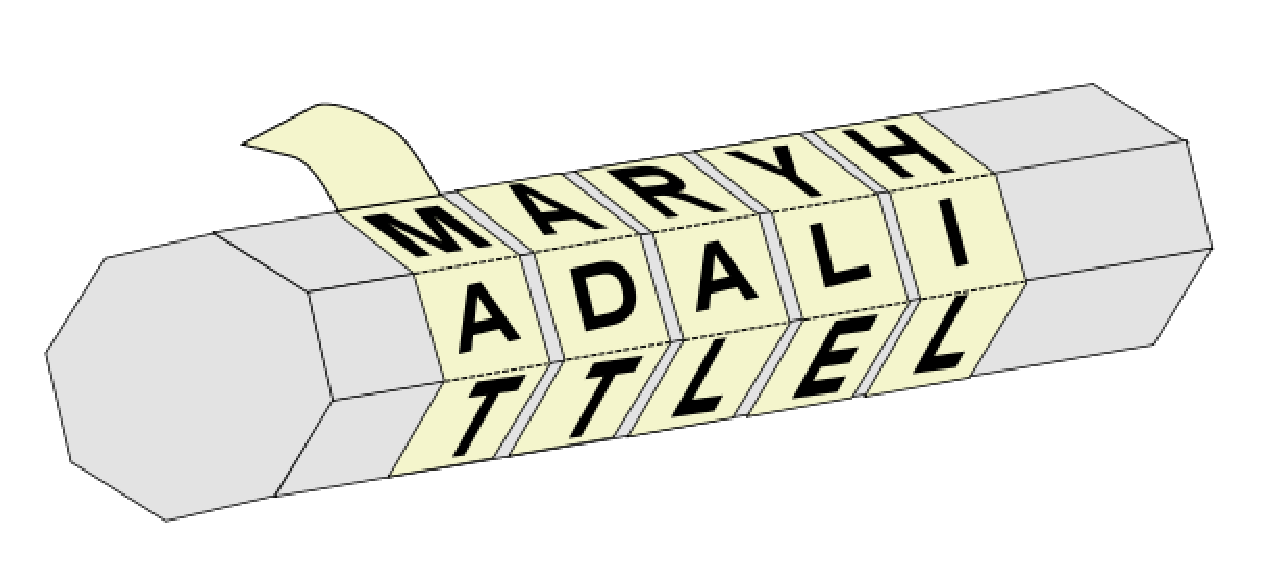
\includegraphics[width=12cm]{Scytale.eps}
 \caption{Sebuah scytale sedang digunakan.\protect\footnotemark}
 \label{fig:scytale}
\end{figure}

\footnotetext{Gambar oleh DMGualtieri, CC BY-SA 3.0
{\tt http://creativecommons.org/licenses/by-sa/3.0},~melalui Wikimedia Commons,
diunduh dari {\tt https://commons.wikimedia.org/wiki/File\%3AScytale.png}}

Di tempat tujuan, dengan asumsi penerima juga mempunyai scytale, pesan akan
muncul kembali seolah-olah secara ajaib ketika lembaran itu dililitkan secara
spiral dan dibaca memanjang.

\ \vskip1mm

\begin{discussion}
Sebelum melanjutkan, kita memerlukan beberapa istilah teknis lagi.
\end{discussion}
\begin{definition}
\label{def:clearplaintext}
\index{teks terang}\index{plainteks}
Pesan yang hendak dikirim Alice kepada Bob dalam bentuk aslinya (dan bentuk
akhir yang dipulihkan) disebut {\bf plainteks} atau {\bf teks terang}.
\end{definition}
\begin{definition}\label{def:encryptioncipher}
\index{enkripsi}\index{cipher}
Algoritme yang digunakan Alice untuk mengubah (mengaburkan) plainteks menjadi
bentuk yang tetap rahasia sekalipun diamati Eve selama pengiriman disebut
{\bf cipher} atau algoritme sandi. Kita juga mengatakan bahwa Alice
{\bf mengenkripsi} pesan (plainteks) tersebut.
\end{definition}
\begin{definition}\label{def:ciphertext}
\index{cipherteks}
Setelah dienkripsi, pesan tersebut disebut {\bf cipherteks} atau
{\bf teks sandi}.
\end{definition}
\begin{definition}\label{def:decrypt}
\index{dekripsi}
Ketika menerima cipherteks, Bob menerapkan algoritme lain untuk
{\bf mendekripsinya} dan memulihkan plainteks.
\end{definition}

\pagebreak
\begin{discussion}
Secara grafis:
\end{discussion}
\begin{center}
\begin{tabular}{|c|c|c|}
\multicolumn{3}{l}{\bf\ \ \ Istilah dasar kripto:}\\
\hline
Alice  & pada jaringan publik & Bob \\
\hline
{\bf plainteks}/{\bf teks terang} & & \\
pesan $m$  & & \\
{\bf mengenkripsi} $m$ menjadi $c$& &\\
mengirim $c$ & \ \quad$\rightarrowtail\ \ \ ${\bf cipherteks}\ $c\ \ \ \rightarrowtail$\quad\  & menerima $c$\\
& & {\bf mendekripsi} $c$ untuk\\
& & memulihkan plainteks $m$\\
\hline
\end{tabular}
\end{center}
\begin{discussion}

\ \vskip1mm

Andaikan seorang mata-mata melihat para pengintai di lapangan melilitkan
lembaran perkamen pada tombak dan menulis sepanjang tombak itu. Artinya, Eve
mengetahui algoritme enkripsinya. Meskipun {\it algoritmenya} diketahui,
kerahasiaan masih mungkin dipertahankan.
\end{discussion}
\begin{definition}\label{def:key}
\index{kunci}
Informasi tambahan---sebagian digunakan dalam enkripsi dan sebagian diperlukan
agar dekripsi berhasil---disebut {\bf kunci}.
\end{definition}
\begin{discussion}

Dalam enkripsi menggunakan scytale, diameter scytale merupakan kuncinya. Bahkan,
ada dugaan bahwa scytale juga berfungsi sebagai bentuk autentikasi sederhana:
hanya Alice yang mempunyai scytale yang cocok dengan milik Bob. Jadi, jika Bob
dapat membaca rangkaian huruf yang bermakna di sepanjang scytale miliknya, ia
mengetahui bahwa Alice-lah yang mengirimkannya.

Bahkan dengan kunci, kelemahan kriptosistem ini cukup jelas. Dan Athena memang
kalah dalam Perang Peloponnesos.

\ \vskip1mm

Pengalaman kriptologi selama berabad-abad menunjukkan bahwa algoritme suatu
kriptosistem justru sebaiknya dibuka kepada publik, sedangkan hanya kunci bagi
saluran komunikasi tertentu (misalnya antara Alice dan Bob) yang dirahasiakan.
Ada banyak alasan untuk pendekatan ini. Alasan utamanya barangkali adalah bahwa
pembuat kriptosistem tidak pernah dapat memastikan bahwa ia telah memikirkan
semua metode kriptanalisis yang mungkin digunakan untuk menyerang sistemnya.
Karena itu, lebih baik pembuat sistem membiarkan komunitas kripto seluas-luasnya
menguji sistem tersebut, dan hanya sistem yang telah bertahan terhadap serangan
semacam itu yang patut digunakan. Bagaimanapun, inilah dasar metode ilmiah:
ilmuwan menerbitkan seluruh rincian eksperimennya agar orang lain dapat
mencobanya, memberikan verifikasi independen, atau menemukan sesuatu yang
perlu dikritik.

\end{discussion}
Gagasan bahwa keamanan kriptosistem harus bertumpu pada kerahasiaan kunci,
bukan kerahasiaan algoritme, dikenal sebagai {\bf Prinsip Kerckhoffs}
\index{Prinsip Kerckhoffs}. Nama itu merujuk pada gagasan perancangan
kriptosistem yang ditulis Auguste Kerckhoffs pada tahun 1883 dalam karya dua
bagiannya, {\it La Cryptographie militaire}. Prinsip ini berlawanan dengan
kriptosistem yang dianggap sangat lemah karena bergantung pada harapan bahwa
algoritmenya tidak akan pernah diketahui. Sistem semacam itu bertumpu pada
paradigma {\bf keamanan melalui ketertutupan} ({\it security through obscurity})
yang tidak bijaksana.\index{keamanan melalui ketertutupan}

\ifdefined\suppressallexercises
  {}
\else
  \vfill
  \pagebreak
  \subsection*{Latihan untuk \S\ref{sec:SSH}}
\fi

\begin{exercise}
Andaikan, untuk suatu $k\in\NN$, plainteks yang hendak dikirim Alice terdiri
atas simbol-simbol $m_1,\dots,m_k$. Andaikan diameter scytale yang digunakannya
memungkinkan $s\in\NN$ huruf ditulis pada setiap putaran spiral perkamen ketika
perkamen itu dililitkan pada scytale.

Tuliskan satu atau beberapa rumus yang mendeskripsikan huruf-huruf
$c_1,\dots,c_k$ dalam cipherteks. Anda harus mengandaikan $s<k$ dan, jika
diinginkan, boleh mengandaikan hubungan tertentu yang berguna, seperti
$s\mid k$.
\end{exercise}
\begin{exercise}
Sekalipun kriptosistem scytale kuat, penggunaannya untuk {\it autentikasi}
mungkin bermasalah. Jelaskan bagaimana autentikasi dapat gagal bergantung pada
pesan yang dikirim; berikan satu atau dua contoh pesan yang ``buruk'' untuk
autentikasi.
\end{exercise}
\begin{exercise}
Kriptosistem scytale tampak lemah. Jelaskan bagaimana Anda akan melakukan
kriptanalisis terhadapnya.
\end{exercise}

\vfill
\pagebreak
\ifdefined\boundarysixteen
  \def\finishboundarysixteen{\backmatter
    \bibliographystyle{amsalpha}
    \bibliography{refs}
    \printindex
    \end{document}}
\else
  \let\finishboundarysixteen\relax
\fi
\finishboundarysixteen
\section{Cipher Caesar dan Varian-Variannya}\label{sec:CCaIV}

\begin{discussion}
Sistem lain yang berasal dari zaman kuno konon digunakan oleh Julius Caesar.
\end{discussion}
\begin{definition}
\label{def:caesarcipher}
\index{cipher Caesar!definisi}
Alice mengambil pesannya, menghapus semua spasi dan tanda baca, lalu menyamakan
kapitalisasi seluruh hurufnya (misalnya menjadi huruf kapital). Kemudian ia
menggeser setiap huruf sejauh $k$ posisi ke depan dalam alfabet, kembali dari Z
ke A jika perlu. Di sini $k\in\ZZ$ adalah bilangan tetap yang hanya diketahui
Alice dan Bob serta disebut {\bf kunci}.

Untuk mendekripsi, Bob cukup menggeser setiap huruf sejauh $k$ posisi ke belakang
dalam alfabet, kembali dari A ke Z jika perlu. Dengan kata lain, Bob mengenkripsi
cipherteks menggunakan kunci $-k$ untuk memperoleh plainteks.

Sistem ini disebut {\bf kriptosistem Caesar}.
\end{definition}
\begin{discussion}

Julius Caesar\index{Julius Caesar} tampaknya biasa menggunakan nilai kunci
$k=3$. Octavian\index{Octavian (Augustus)}, cucu dari saudari Julius Caesar,
kemudian menjadi Kaisar Augustus\index{Augustus} dan suka menggunakan $k=-1$.

Jika kita menggunakan apa yang disebut alfabet Latin (meskipun alfabet ini
bukan alfabet yang digunakan di Romawi kuno) dengan 26 huruf, ada satu nilai
kunci yang sangat menarik: 13. Dengan nilai itu, enkripsi dan dekripsi merupakan
transformasi yang persis sama. Pada zaman modern, transformasi ini disebut
{\bf ROT13}\index{ROT13}, dan pernah memainkan peran kecil dalam sejarah modern
Internet. Misalnya, kiriman di ruang obrolan dan papan buletin awal kadang-kadang
memuat bagian yang tidak boleh langsung terlihat oleh siapa saja yang membaca
kiriman, tetapi tetap dapat dibuka oleh pembaca yang bersungguh-sungguh (seperti
bocoran alur dalam ulasan gim, buku, atau film baru yang populer). Bagian semacam itu
sering disertakan setelah terlebih dahulu diproses dengan ROT13.

Walaupun sebenarnya sama sekali tidak aman, ROT13 bahkan pernah digunakan untuk
tujuan keamanan yang sesungguhnya dalam beberapa produk komersial, termasuk
pada bagian tertentu dari beberapa versi sistem operasi Windows.

\ \vskip1mm

Cipher Caesar sudah berhasil dipecahkan sepenuhnya (dengan beberapa cara; lihat
\S\ref{sec:FSiCFA} di bawah) sebelum tahun 1000 M, tetapi salah satu turunannya
dikembangkan pada akhir Abad Pertengahan dan dianggap sebagai teknologi
kriptologi termaju hingga awal zaman modern.

\end{discussion}
\begin{definition}
\label{def:vigenerecipher}
\index{cipher Vigen\`ere}
Sekali lagi, Alice mengambil pesannya, menghapus semua spasi dan tanda baca,
lalu menyamakan kapitalisasi seluruh hurufnya (misalnya menjadi huruf kapital).
Kali ini, kunci $\vec{k}=(k_1,\dots,k_\ell)$ yang dimiliki bersama oleh Alice
dan Bob merupakan tupel-$\ell$, untuk $\ell\in\NN$, yang terdiri atas bilangan
bulat $k_1,\dots,k_\ell\in\ZZ$.

Untuk mengenkripsi, Alice menelusuri pesan plainteks dan barisan kuncinya
bersama-sama, satu huruf demi satu huruf. Setiap huruf plainteks digeser ke depan
(kembali dari Z ke A jika perlu) sebanyak bilangan yang ditentukan oleh komponen
kunci yang bersesuaian. Jika komponen kuncinya habis, Alice kembali ke awal
barisan kunci.

Untuk mendekripsi, Bob menggeser setiap huruf ke belakang sesuai komponen kunci
yang bersesuaian, kembali dari A ke Z jika perlu. Dengan kata lain, Bob
mengenkripsi menggunakan kunci
$-\vec{k}=(-k_1,\dots,-k_\ell)$.

Sistem ini disebut {\bf kriptosistem Vigen\`ere}.
\end{definition}
\begin{discussion}

Secara tradisional, kunci Vigen\`ere berupa sebuah kata yang dituliskan,
dihafalkan, dan dimiliki bersama oleh Alice dan Bob. Ketika mengenkripsi atau
mendekripsi, huruf-huruf kata kunci itu ``ditambahkan'' pada huruf-huruf pesan
seperti dijelaskan di atas, dengan konvensi $A=1$, $B=2$, dan seterusnya.

Perhatikan bahwa Vigen\`ere dengan panjang kunci $\ell$ pada dasarnya merupakan
$\ell$ cipher Caesar yang berjalan paralel. Bahkan, jika $\ell=1$, keduanya
merupakan kriptosistem yang persis sama. Karena itu, Vigen\`ere pada dasarnya
$\ell+1$ kali lebih sulit dipecahkan daripada Caesar; suku ``${}+1$'' muncul
karena Eve bahkan tidak mengetahui $\ell$. Meskipun demikian, setelah beberapa
ratus tahun dianggap tidak dapat dipecahkan dan digunakan sebagai cipher
diplomatik utama di istana-istana Eropa, metode untuk memecahkan Vigen\`ere
akhirnya dikembangkan.

\ \vskip1mm

Sebagai varian terakhir cipher Vigen\`ere, andaikan kita bergerak ke arah yang
berlawanan dari kasus ekstrem $\ell=1$ dan memilih $\ell$ sepanjang mungkin.

\end{discussion}
\begin{definition}
\label{def:onetimepad}
\index{pad sekali pakai}
{\bf Pad sekali pakai} ({\it one-time pad}) adalah kriptosistem Vigen\`ere yang
kuncinya sama panjang dengan pesan, dipilih secara acak, dan tidak pernah
digunakan kembali. [Kunci dalam kriptosistem ini juga disebut {\it pad sekali
pakai}\footnote{Sinekdoke lagi!}.]
\end{definition}
\begin{discussion}

(Pad sekali pakai kadang-kadang disebut {\it Cipher Vernam}
\index{Cipher Vernam}. Sebutan ini tidak tepat jika dilihat dari sejarah
intelektual kriptosistem yang sebenarnya.)

Barisan kunci yang baik sangat penting dalam kriptosistem pad sekali pakai.
Kabar baiknya, dapat dibuktikan bahwa jika pad sekali pakai benar-benar acak,
kriptosistem yang dihasilkan memang aman secara sempurna. Dalam ilmu komputer,
sifat ini disebut {\it aman secara teori informasi}
\index{aman secara teori informasi}, sebab bukti keamanannya tidak bergantung
pada asumsi apa pun tentang sumber daya komputasi yang tersedia bagi penyerang.
[Lihat \cite{shannon1949communication} dan \cite{shannon1948mathematical} untuk
bukti tersebut.] Kriptosistem lain yang akan kita jumpai di bawah hanya aman
jika kita mengandaikan bahwa penyerang mempunyai akses ke komputer jenis
tertentu (asumsi yang lazim ialah sebuah {\it mesin Turing waktu-polinomial
probabilistik}\index{mesin Turing waktu-polinomial probabilistik}; bidang ilmu
komputer yang membahas hal ini disebut {\it kompleksitas komputasi}; lihat,
misalnya, \cite{arora2009computational}).

Pad yang sama juga tidak boleh digunakan lebih dari sekali. Jika digunakan
kembali, penyerang dapat mengambil selisih kedua cipherteks huruf demi huruf,
yang akan meniadakan pad sepenuhnya dari perhitungan. Setelah itu, pesan biasanya
dapat ditentukan dengan cepat.

Pada zaman modern, setelah munculnya jaringan komunikasi digital, pesan ditulis
sebagai data komputer. Dengan demikian, semuanya disimpan (dan dikirimkan)
sebagai bit, yaitu $1$ dan $0$. Untuk bit, padanan penggeseran huruf dalam
alfabet dengan kembali dari Z ke A bila perlu adalah: tidak melakukan apa pun
jika besar pergeserannya genap, atau menukar $0$ dan $1$ jika pergeserannya
ganjil.

Dengan kata lain, jika pesan dan kunci sama-sama dituliskan seluruhnya sebagai
bit---anggap setiap bit sebagai salah satu dari elemen
$[0],[1]\in\ZZ/2\ZZ$---enkripsi tepat
berupa penjumlahan bit-bit yang bersesuaian modulo $2$. Karena itu, pad sekali
pakai yang baik merupakan untaian bit (kelas-kelas kongruensi dalam
$\ZZ/2\ZZ$) yang sangat acak dan sangat panjang.

Masalah besar pad sekali pakai adalah {\it distribusi kunci:}
\index{distribusi kunci} Alice dan Bob harus sudah memiliki bersama pad sekali
pakai yang sangat besar sebelum mulai berkomunikasi. Panjangnya harus
sekurang-kurangnya sama dengan jumlah seluruh huruf (atau bit pada zaman
komputer) dalam semua pesan yang akan mereka kirim pada masa depan.

Hal ini menyarankan pendekatan menarik terhadap kriptografi: carilah cara agar
Alice dan Bob dapat berbagi sebuah rahasia kecil yang memungkinkan keduanya
menghasilkan barisan bit sepanjang apa pun, memperoleh barisan yang sama, tetapi
barisan itu tampak sepenuhnya acak bagi setiap penyerang. Jika hal ini mungkin,
mereka dapat menggunakan barisan {\it acak semu}\index{acak semu} tersebut
sebagai pad sekali pakai. Disebut acak semu karena barisan itu sebenarnya tidak
acak---Alice dan Bob dapat menentukannya terlebih dahulu dari rahasia awal yang
kecil---tetapi bagi semua penyerang barisan itu tampak acak. [Lihat
\cite{luby1996pseudorandomness} untuk pembahasan lebih lanjut tentang keacakan
semu.]
\end{discussion}

\ifdefined\suppressallexercises
  {}
\else
  \vfill
  \pagebreak
  \subsection*{Latihan untuk \S\ref{sec:CCaIV}}
\fi

\begin{exercise}
ROT13 dianggap menarik karena mengurangi banyaknya kode yang perlu dibuat:
program yang sama dapat melakukan dekripsi maupun enkripsi, sebab penerapan
ROT13 untuk kedua kalinya membatalkan transformasi ROT13 yang pertama.

Apakah hal yang sama berlaku untuk cipher Caesar berkunci lainnya? Buatlah
konjektur tentang apakah, untuk suatu kunci cipher Caesar $k\in\ZZ$ dan pesan
$m$, selalu terdapat $n\in\NN$ sedemikian sehingga
$$
\overbrace{e^C_k\circ\dots\circ e^C_k}^{\text{$n$ kali}}(m)=m
$$
di mana $e^C_k$ adalah fungsi enkripsi Caesar dengan kunci $k$. Jika ya,
carilah rumus untuk $n$ terkecil semacam itu, yang boleh bergantung (jika perlu)
pada $k$, $m$, dan banyaknya huruf dalam alfabet yang digunakan untuk menulis
$m$.
\end{exercise}

\begin{exercise}
Lanjutkan latihan sebelumnya. Sekarang andaikan
$\vec{k}=(k_1,\dots,k_\ell)$ merupakan tupel-$\ell$, untuk $\ell\in\NN$, yang
terdiri atas bilangan bulat $k_1,\dots,k_\ell\in\ZZ$, dan
$e^V_{\vec{k}}$ adalah fungsi enkripsi Vigen\`ere dengan kunci $\vec{k}$.
Tentukan apakah, untuk setiap pesan $m$, terdapat $n\in\NN$ sedemikian sehingga
$$
\overbrace{e^V_{\vec{k}}\circ\dots\circ e^V_{\vec{k}}}^{\text{$n$ kali}}(m)=m
$$
dan, jika ya, carilah rumus untuk $n$ terkecil semacam itu, yang boleh
bergantung (jika perlu) pada $\vec{k}$, $m$, dan banyaknya huruf dalam alfabet
yang digunakan untuk menulis $m$.
\end{exercise}

\begin{exercise}
Andaikan Eve mempunyai kembaran bernama Vev. Keduanya mengamati
cipherteks $c$ yang dikirim Alice kepada Bob dan berhasil mereka cegat. Mereka
menduga bahwa pasangan kekasih konyol Alice dan Bob menggunakan pad sekali
pakai untuk mengenkripsi komunikasi mereka. Eve dan Vev sama-sama melakukan
banyak perhitungan dan mengira telah berhasil mendekripsi $c$ dengan benar.
Sayangnya, Eve dan Vev masing-masing memperoleh nilai $m_e$ dan $m_v$ yang
berbeda (dan keduanya bermakna!), lalu menganggap nilainya sebagai plainteks
yang hendak dikirim Alice kepada Bob.

Pad sekali pakai $p_e$ dan $p_v$ apakah yang, menurut perhitungan (atau tebakan)
mereka masing-masing, digunakan Alice?

Apakah hasil dekripsi usulan $m_e$ dan $m_v$ dapat dipilih sembarang, atau adakah
hubungan antara kedua hasil dekripsi usulan, pad usulan $p_e$ dan $p_v$,
plainteks sebenarnya, serta pad sekali pakai yang benar-benar digunakan Alice?

Kerjakan satu contoh konkret. Jika pesan teks terang asli Alice $m$ adalah
{\tt aardvark}, mungkinkah Eve mengira pesannya
$m_e=$~{\tt iloveyou}, sedangkan Vev mengira pesannya
$m_v=$~{\tt ihateyou}? Jika mungkin, berikan contoh cipherteks $c$ yang
bersesuaian, pad sekali pakai Alice dan Bob $p_{AB}$, hasil dekripsi usulan
$m_e$ dan $m_v$, serta pad sekali pakai usulan $p_e$ dan $p_v$.
\end{exercise}

\vfill
\pagebreak
\ifdefined\boundaryseventeen
  \def\finishboundaryseventeen{\backmatter
    \bibliographystyle{amsalpha}
    \bibliography{refs}
    \printindex
    \end{document}}
\else
  \let\finishboundaryseventeen\relax
\fi
\finishboundaryseventeen
\section{Langkah Awal dalam Kriptanalisis: Analisis Frekuensi}
\label{sec:FSiCFA}

\begin{discussion}
Cipher Caesar tampak sangat lemah. Namun, ketika kita melihat suatu cipherteks,
seperti
\begin{verbatim}
            wrehruqrwwrehwkdwlvwkhtxhvwlrq
            zkhwkhuwlvqreohulqwkhplqgwrvxiihu
            wkhvolqjvdqgduurzvrirxwudjhrxviruwxqh
            ruwrwdnhdupvdjdlqvwdvhdriwurxeohv
            dqgebrssrvlqjhqgwkhp
\end{verbatim}
sulit untuk mengetahui harus mulai dari mana---teks itu nyaris sama sekali
tidak tampak seperti bahasa Inggris.

Mungkin kita perlu mulai dari cipher Caesar itu sendiri, dengan mengandaikan
(secara anakronistis) bahwa Caesar mengikuti Prinsip Kerckhoffs, atau (lebih
sesuai dengan zamannya) bahwa para mata-mata telah mengetahui kriptosistemnya
tetapi belum mengetahui kuncinya.

Kita segera menyadari bahwa hal yang tidak diketahui, yaitu kunci, begitu kecil
dibandingkan dengan kesulitan yang ditimbulkannya. Bahkan, jika kita memilih
kunci secara acak, hampir empat dari 100 percobaan akan menghasilkan dekripsi
yang benar semata-mata karena keberuntungan. Perhitungan ini menggunakan
``alfabet Latin'' modern yang terdiri atas 26 huruf; pada zaman Caesar,
alfabet Latin yang sebenarnya hanya memiliki 23 huruf, sehingga peluangnya
bahkan lebih baik. Secara formal, kita membicarakan konsep berikut.
\end{discussion}
\begin{definition}\label{def:keyspace}\index{ruang kunci}
Himpunan semua kunci yang sah untuk suatu kriptosistem disebut
{\bf ruang kunci}.
\end{definition}
\begin{example}\label{eg:keyspaceCaesar}
Ruang kunci kriptosistem cipher Caesar adalah alfabetnya.
\end{example}
\begin{example}\label{eg:keyspaceVigenere}
Ruang kunci kriptosistem cipher Vigen\`ere dengan panjang kunci $\ell$ adalah
semua barisan yang terdiri atas $\ell$ huruf dalam alfabet. Karena itu, ruang
tersebut memiliki $N^\ell$ elemen jika alfabetnya berukuran $N$. Jika panjang
kunci yang tepat tidak diketahui, tetapi diketahui tidak melebihi suatu batas
$L\in\NN$, terdapat $\sum_{j=1}^L N^j$ kemungkinan kunci.
\end{example}
\begin{example}\label{eg:keyspaceOTP}
Setiap barisan huruf sepanjang $M$ merupakan kemungkinan kunci (pad) untuk
enkripsi pad sekali pakai atas pesan sepanjang $M$. Karena itu, terdapat $N^M$
kemungkinan pad sekali pakai untuk pesan sepanjang $M$ pada alfabet berukuran
$N$.
\end{example}

\begin{discussion}
Kita menghitung ukuran berbagai ruang kunci tersebut karena salah satu
kelemahan cipher Caesar adalah ruang kuncinya yang begitu kecil. Strategi yang
lebih baik daripada menebak secara acak ialah mencoba semua kunci yang mungkin
dan melihat kunci mana yang menghasilkan dekripsi yang benar. Hanya ada 26
kunci (atau 23 pada zaman Julius)! Pendekatan ini disebut {\it serangan brute
force} [atau {\it pencarian menyeluruh}].\index{serangan brute force}
\index{pencarian menyeluruh} Bahkan pada zaman Caesar, ruang kunci cipher Caesar
sudah begitu kecil sehingga Eve dapat memeriksa semua kunci dan melihat kunci
mana yang menghasilkan teks terang pesan Alice kepada Bob.

Cipher Vigen\`ere sedikit lebih sulit. Sebagai contoh, jika panjang kunci
diketahui sama dengan lima, hampir 12 juta kunci harus dicoba. Sebelum zaman
komputer, pekerjaan ini sama sekali tidak mungkin ditangani. Bahkan pada abad
ke-21, ketika komputer dapat menghasilkan semua kemungkinan dekripsi itu dalam
waktu yang bagi manusia tampak seketika, masih ada masalah: manusia harus
memeriksa 12 juta kemungkinan tersebut dan memilih dekripsi yang sah.

{\it Mechanical Turk} milik Amazon (lihat
{\tt https://www.mturk.com/mturk/welcome})\index{Mechanical Turk} mungkin dapat
menghimpun cukup banyak tenaga manusia untuk menyelesaikan satu dekripsi
Vigen\`ere dengan brute force. Namun, pendekatan yang lebih baik ialah menulis
program komputer yang dapat membedakan teks tanpa makna dari pesan nyata yang
mungkin dikirim Alice kepada Bob. Dengan begitu, serangan brute force dapat
berhasil dalam beberapa saat.

Untuk membedakan teks tanpa makna dari pesan nyata, kita perlu mengetahui
pesan-pesan nyata apa saja yang mungkin. Hal ini memotivasi definisi berikut.
\end{discussion}
\begin{definition}\label{def:messagespace}\index{ruang pesan}
Himpunan pesan yang mungkin dalam suatu komunikasi terenkripsi disebut
{\bf ruang pesan}.
\end{definition}
\begin{discussion}
Tanpa suatu struktur pada ruang pesan, kriptanalisis dapat menjadi nyaris
mustahil. Misalnya, jika Alice mengirimkan kode kombinasi sebuah brankas kepada
Bob melalui surel dalam bentuk terenkripsi, ruang pesannya tidak terlalu besar
tetapi tidak mempunyai ciri yang dapat dikenali. Serangan brute force tidak
memiliki cara untuk menentukan hasil dekripsi mana yang merupakan kode
kombinasi sebenarnya.

Namun, andaikan ruang pesan komunikasi Alice dan Bob berupa himpunan teks pendek
(atau panjang, yang lebih baik) dalam bahasa Inggris. Teks bahasa Inggris
mempunyai cukup banyak struktur; manusia penutur bahasa Inggris tentu dapat
mengenali bahasa Inggris yang wajar. Pertanyaannya ialah apakah proses
mendeteksi teks bahasa Inggris yang wajar dapat diotomatisasi.

Mari kita lihat kembali contoh enkripsi Caesar pada awal bagian ini. Kita sudah
melihat bahwa hasilnya tidak tampak seperti bahasa Inggris---tetapi dalam hal
apa? Salah satunya tentu karena teks itu tidak memuat kata bahasa Inggris.
Orang yang mengetahui bahasa Inggris mengenal sebagian besar kosakatanya dan
dapat melihat bahwa teks tersebut tidak memuat kata-kata itu, kecuali mungkin
``up'' dan ``i'' (beberapa kali).

Hal ini menyarankan sebuah pendekatan: ambil daftar semua kata bahasa Inggris
beserta semua bentuk varian dan turunannya; tambahkan beberapa barisan acak
pendek yang mungkin muncul di dalam bahasa Inggris baku (misalnya ketika Alice
mengutip ucapan tanpa makna yang didengarnya atau menyalin grafiti pada sisi
gerbong kereta bawah tanah); lalu bandingkan daftar itu dengan semua kemungkinan
dekripsi cipherteks. Skema ini tidak terlalu praktis. Namun, jika ruang pesannya
cukup kecil, pendekatan semacam ini masuk akal.

Jika kita kembali melihat pesan tersebut, pembaca bahasa Inggris juga segera
merasa bahwa huruf atau kombinasi hurufnya tidak tepat. Misalnya, tampaknya tidak
ada cukup banyak vokal. Pemeriksaan seberapa sering huruf muncul dalam sebuah
teks dibandingkan dengan frekuensi yang diharapkan disebut {\it analisis
frekuensi}.\index{analisis frekuensi} Penggunaannya dalam kriptanalisis
tampaknya pertama kali dijelaskan oleh filsuf dan matematikawan Muslim al-Kindi
\footnote{Al-Kindi adalah tokoh yang sangat menarik dalam sejarah intelektual
Muslim awal. Sebagai contoh, tampaknya ia memperkenalkan bilangan Hindu beserta
notasi nilai tempatnya ke dunia Muslim.}\index{al-Kindi} dalam karyanya pada
abad ke-9, {\it Manuskrip tentang Penguraian Pesan Kriptografis}.

Berikut adalah tabel frekuensi huruf dalam sejumlah teks bahasa Inggris baku
(beberapa drama Shakespeare):\index{frekuensi huruf, bahasa Inggris}
\begin{figure}[H]
 \centering
 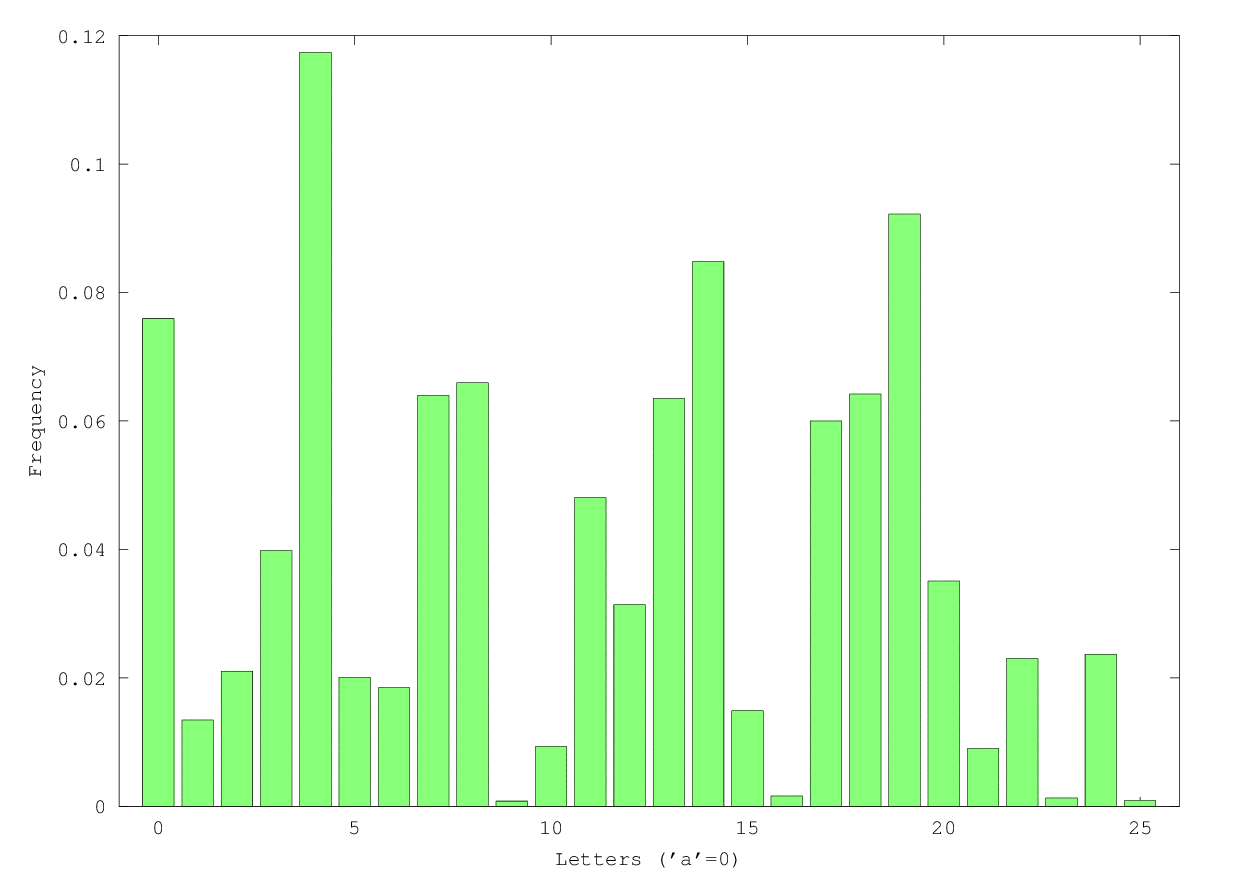
\includegraphics[width=12cm]{eng_freq_hist.eps}
 \caption{Frekuensi huruf dalam beberapa drama Shakespeare}
 \label{fig:eng_freq_hist}
\end{figure}
Perhatikan bahwa huruf `e' merupakan huruf yang paling sering muncul, meskipun
hanya dengan selisih kecil. Jadi, pendekatan kriptanalisis pertama menggunakan
analisis frekuensi dapat dilakukan dengan memilih kunci dekripsi Caesar yang
menggeser huruf paling sering dalam cipherteks menjadi `e'. Untuk cipherteks
pada awal bagian ini, pendekatan tersebut menghasilkan dekripsi:
\begin{verbatim}
            ezmpzcyzeezmpesletdespbfpdetzy
            hspespcetdyzmwpctyespxtyoezdfqqpc
            espdwtyrdlyolcczhdzqzfeclrpzfdqzcefyp
            zcezelvplcxdlrltydeldplzqeczfmwpd
            lyomjzaazdtyrpyoespx
\end{verbatim}
Hasilnya kurang baik. Rupanya, hanya memperhatikan huruf yang paling sering
belum cukup: huruf paling sering dalam plainteks pesan ini bukan `e'.

Sebagai gantinya, mari kita lihat seluruh tabel frekuensi cipherteks ini.
\begin{figure}[H]
 \centering
 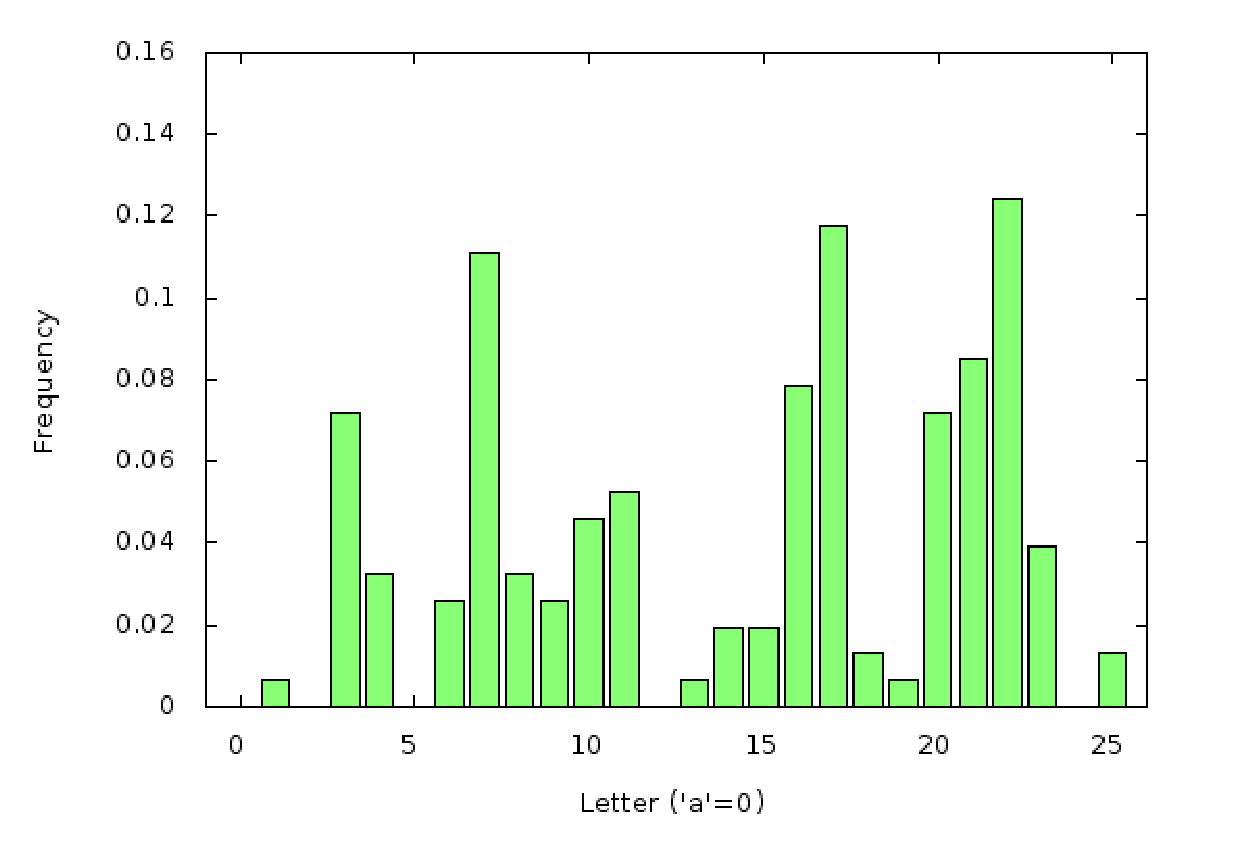
\includegraphics[width=12cm]{samp_Cct_hist.eps}
 \caption{Frekuensi huruf dalam contoh cipherteks Caesar}
 \label{fig:samp_Cct_hist}
\end{figure}
Sayangnya, hasil ini tidak persis sama dengan distribusi frekuensi bahasa
Inggris baku (berdasarkan Shakespeare), bahkan bukan sekadar versi distribusi
Shakespeare yang digeser (dengan kembali dari 25 ke 0). Namun, mungkin salah
satu pergeserannya cukup dekat dengan distribusi Shakespeare.

Hal ini menyarankan pendekatan kriptanalisis yang lebih halus:
\index{cipher Caesar!pemecahan} coba semua kemungkinan dekripsi (tidak terlalu
berat untuk cipher Caesar karena ruang kuncinya kecil), lalu pilih hasil yang
seluruh tabel frekuensi hurufnya paling dekat dengan tabel frekuensi bahasa
Inggris baku. Jadi, kita {\it tidak} hanya melihat huruf yang paling sering,
melainkan seluruh distribusi frekuensinya; dan kita {\it tidak} mencari
kecocokan persis, melainkan kecocokan hampiran terbaik.

Pertanyaan berikutnya ialah cara terbaik untuk mengukur jarak antara dua
distribusi. Salah satu pendekatan yang lazim ialah mengukur besaran berikut.
\end{discussion}
\begin{definition}
\index{jarak antara distribusi frekuensi}\index{galat kuadrat}
{\bf Galat kuadrat total} adalah jarak antara dua distribusi $f$ dan $g$ yang
diberikan oleh
$$
d(f,g)=\sum_{j=0}^{25} \left(f(j)-g(j)\right)^2
$$
di mana distribusi selalu didefinisikan pada huruf dalam bentuk
`a'=0, `b'=1, dan seterusnya.
\end{definition}
\begin{discussion}
Meminimumkan jarak ini ekuivalen dengan metode {\it kuadrat terkecil} dalam
statistika atau aljabar linear.\index{kuadrat terkecil}

Dengan menerapkan strategi ini pada cipherteks dari awal bagian, kita memperoleh
hasil berikut.
\begin{figure}[H]
 \centering
 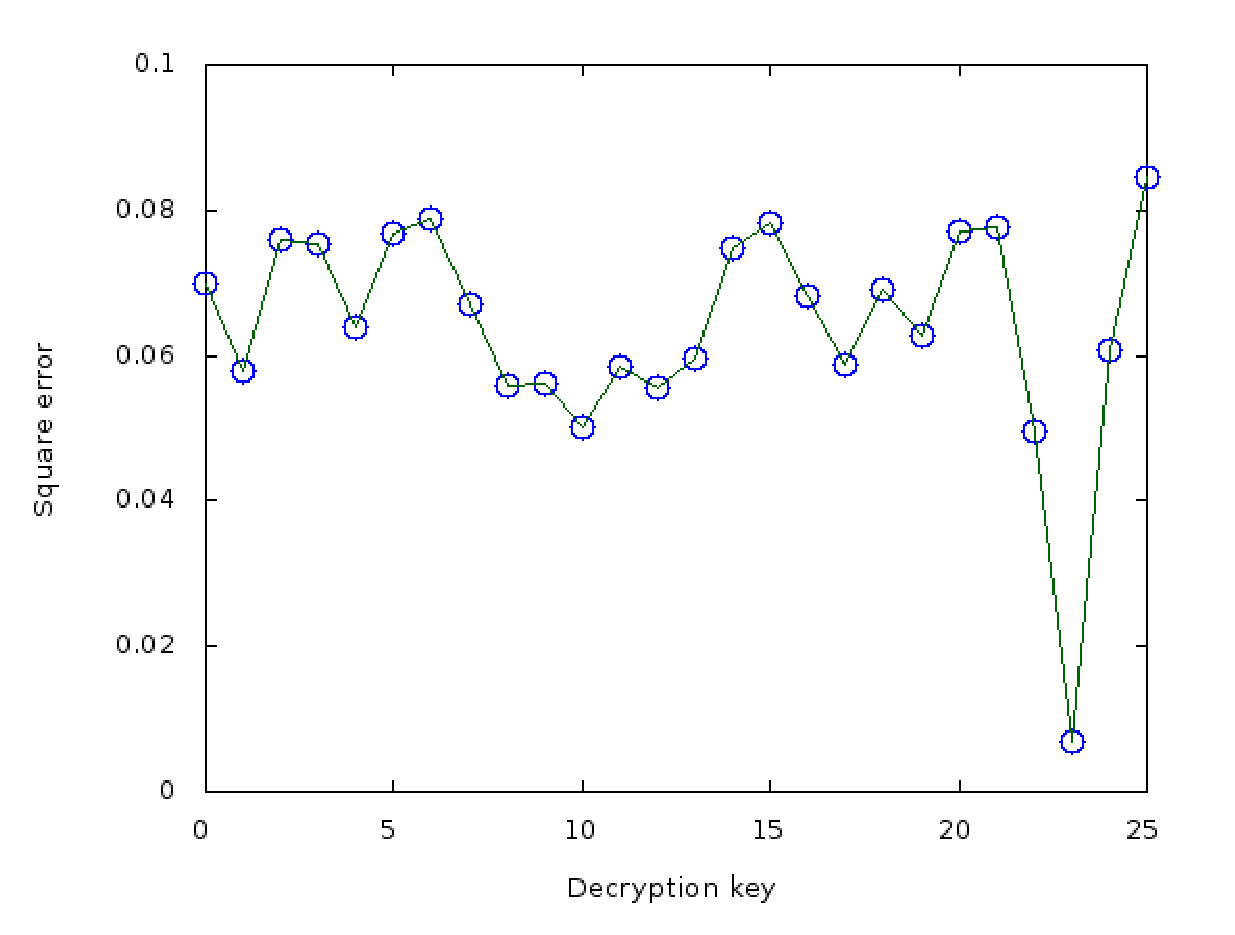
\includegraphics[width=12cm]{seadk_Cct.eps}
 \caption{Galat kuadrat untuk semua kunci dekripsi pada contoh cipherteks Caesar}
 \label{fig:seadk_Cct}
\end{figure}
Galat kuadrat minimum diperoleh dari kunci dekripsi 23 (yang bersesuaian dengan
kunci enkripsi awal 3; secara anakronistis, enkripsi ini dilakukan oleh Julius
sendiri). Teks terang yang bersesuaian adalah
\begin{verbatim}
            tobeornottobethatisthequestion         
            whethertisnoblerinthemindtosuffer
            theslingsandarrowsofoutrageousfortune
            ortotakearmsagainstaseaoftroubles
            andbyopposingendthem
\end{verbatim}
yang tampak cukup meyakinkan.

Menariknya, pendekatan untuk mendeteksi teks bermakna ini cukup tangguh, bahkan
untuk teks sangat pendek yang distribusi frekuensinya mungkin cukup jauh dari
standar bahasa Inggris. Sebagai contoh, untuk cipherteks
\begin{center}
{\tt rkkrtbrkeffespkyvtifjjifruj}
\end{center}
kita memperoleh
\begin{figure}[H]
 \centering
 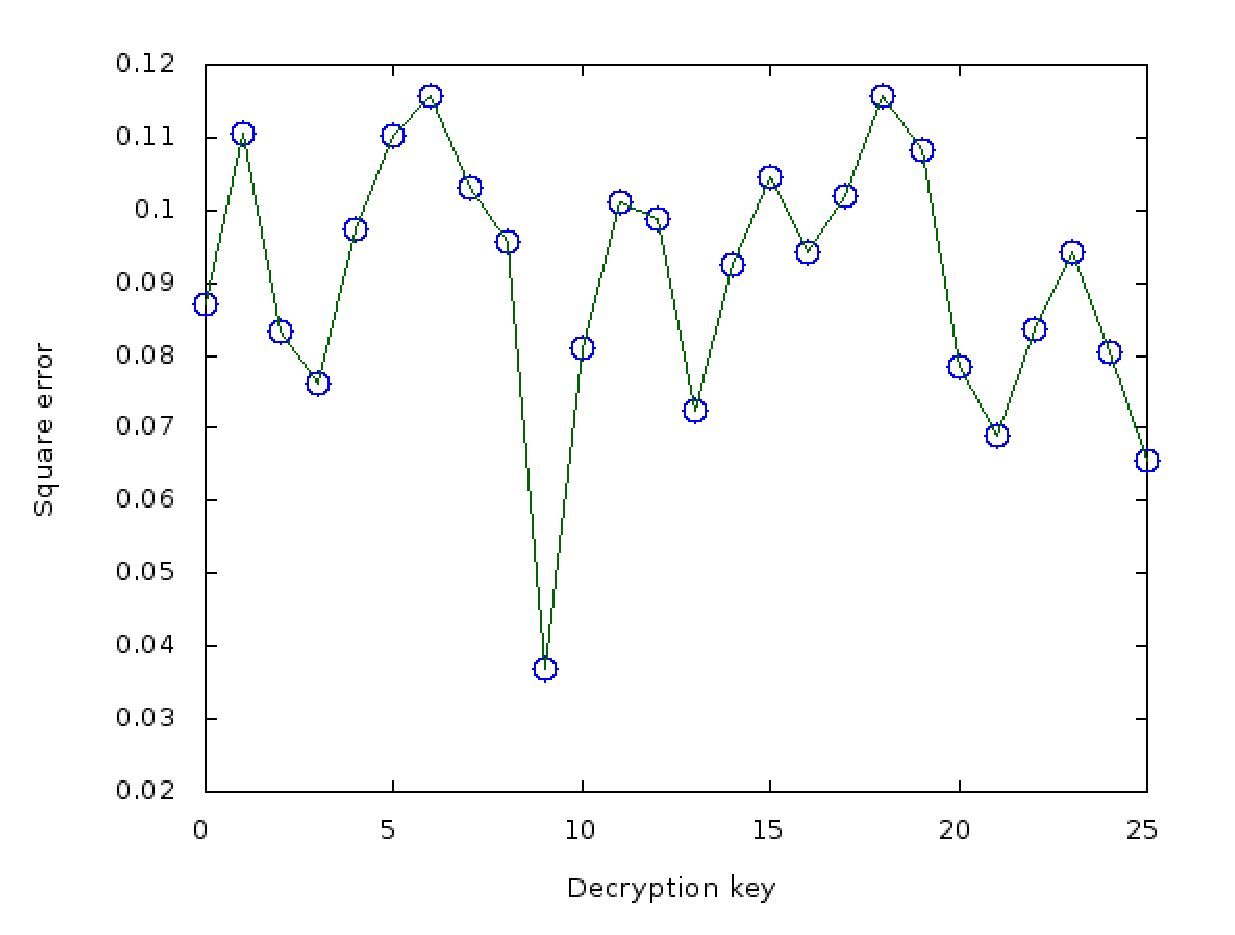
\includegraphics[width=12cm]{seadk_rkkrt.eps}
 \caption{Galat kuadrat untuk semua kunci dekripsi pada cipherteks Caesar
          {\tt rkkrtbrkeffespkyvtifjjifruj}}
 \label{fig:seadk_rkkrt}
\end{figure}
\noindent yang menunjukkan bahwa kunci dekripsinya adalah 9 dan bersesuaian
dengan kunci enkripsi 17. Jadi, teks terangnya pasti
\begin{center}
{\tt attackatnoonbythecrossroads}
\end{center}
yang tampak seperti sesuatu yang mungkin dikatakan Julius.

\ \vskip1mm

Cukup sampai di sini kriptanalisis cipher Caesar. Ketika beralih ke
Vigen\`ere, persoalan pertama adalah menentukan panjang kunci. Jika panjang
kunci $\ell$ diketahui, kita dapat membagi cipherteks menjadi $\ell$ teks yang
lebih pendek: teks pertama memuat karakter-karakter berselang $\ell$ posisi
mulai dari karakter pertama, teks kedua mulai dari karakter kedua, dan
seterusnya, hingga teks yang dimulai dari karakter ke-$\ell$. Dengan menerapkan
pemecah Caesar otomatis yang
dijelaskan di atas, kita memperoleh $\ell$ komponen kunci dan kemudian
plainteksnya.

Untuk mempermudah, andaikan kita mengambil seluruh {\it Hamlet} dan
mengenkripsinya dengan Vigen\`ere menggunakan kata kunci
{\tt hippopotomonstrosesquipedaliophobia}, yang bersesuaian dengan kunci numerik
\begin{align*}
k=(7,8,15,15,14,15,14,19,14,12,14,13,18,19,17,14,\\
18,4,18,16,20,8,15,4,3,0,11,8,14,15,7,14,1,8,0)
\end{align*}
Sebagai contoh, bagian cipherteks yang bersesuaian dengan kutipan untuk
memecahkan cipher Caesar di atas adalah

\vfill
\begin{verbatim}
            hdxajnioomjvdtfvstrqitmfozlxjj
            kcmiosgpenjjbgxmcmtfzltmaudofpmwg
            odsntxuuhwjywmrjpnieosoqlfbpjoqyyljia
            cmbdaozawminabtdhrtyndlncugkflswh
            vjrwgdwddoeicznymcyl
\end{verbatim}
Jika Eve berharap teks ini hanya dienkripsi dengan Caesar, sehingga panjang
kunci Vigen\`ere adalah $\ell=1$, ia akan memperoleh frekuensi huruf berikut.
\begin{figure}[H]
 \centering
 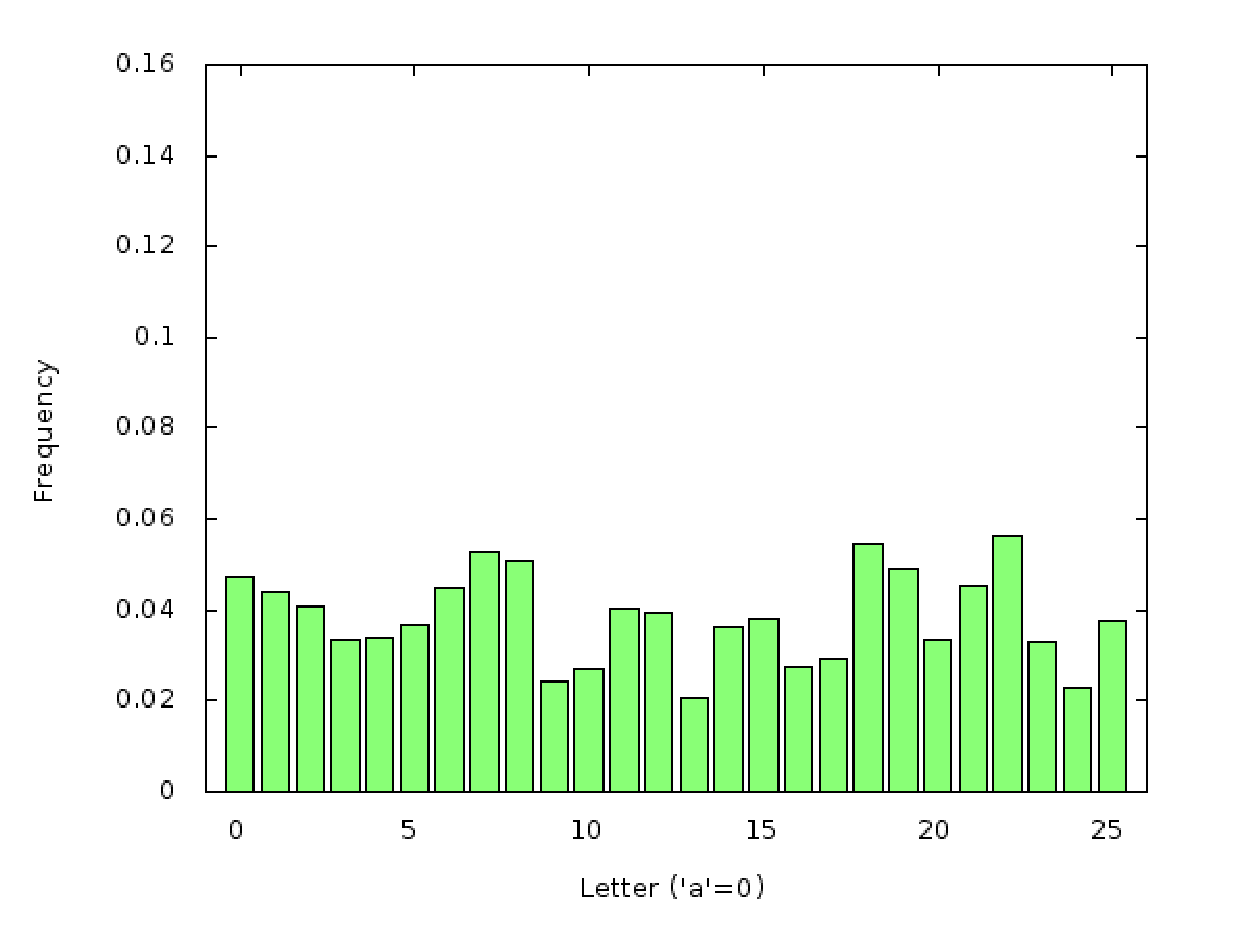
\includegraphics[width=12cm]{hamhip_freqs.eps}
 \caption{Frekuensi huruf dalam enkripsi Vigen\`ere atas {\it Hamlet}
          dengan kunci {\tt hippopotomonstrosesquipedaliophobia}}
 \label{fig:hamhip_freqs}
\end{figure}

\noindent
Dibandingkan dengan Gambar~\ref{fig:samp_Cct_hist}, nilai-nilai ini menunjukkan
variasi yang jauh lebih kecil. Bahkan, tidak ada nilai nol maupun nilai yang
jauh lebih besar daripada semua nilai lainnya. Alasannya, secara hampiran
distribusi ini merupakan campuran dari 35 pergeseran distribusi baku bahasa
Inggris dalam Gambar~\ref{fig:eng_freq_hist}, satu untuk setiap posisi kata kunci
{\tt hippopotomonstrosesquipedaliophobia}; jika pergeseran yang sama digabungkan,
hasilnya adalah campuran berbobot dari 16 nilai pergeseran berbeda. Pencampuran
ini menghaluskan seluruh
bentuk khas distribusi yang berguna untuk mengenali pergeseran dekripsi yang
benar.

Meskipun demikian, pemecah Caesar akan menghasilkan suatu nilai kunci untuk
setiap kemungkinan nilai $\ell$ yang dicoba Eve. Untuk setiap posisi kunci,
selalu ada nilai pergeseran yang meminimumkan galat kuadrat. Jika tebakan
panjang kunci $\ell$ salah dan pengelompokan yang dihasilkan mencampurkan
beberapa pergeseran berbeda, nilai minimum ini biasanya tidak terlalu kecil:
distribusi frekuensi huruf pada posisi-posisi cipherteks yang kongruen dengan
$k\pmod{\ell}$, untuk $k\in\NN$ dan $k\le\ell$, biasanya lebih datar, sehingga
jauh (menurut jarak galat kuadrat) dari distribusi bahasa Inggris baku.

Sebagai contoh, pada enkripsi {\it Hamlet} yang sedang kita kaji, andaikan Eve
menebak $\ell=5$ dan mengambil semua huruf pada posisi yang kongruen dengan
$1\pmod{5}$. Pemecah Caesar akan menghasilkan grafik galat kuadrat
berikut:\newline
\begin{figure}[H]
 \centering
 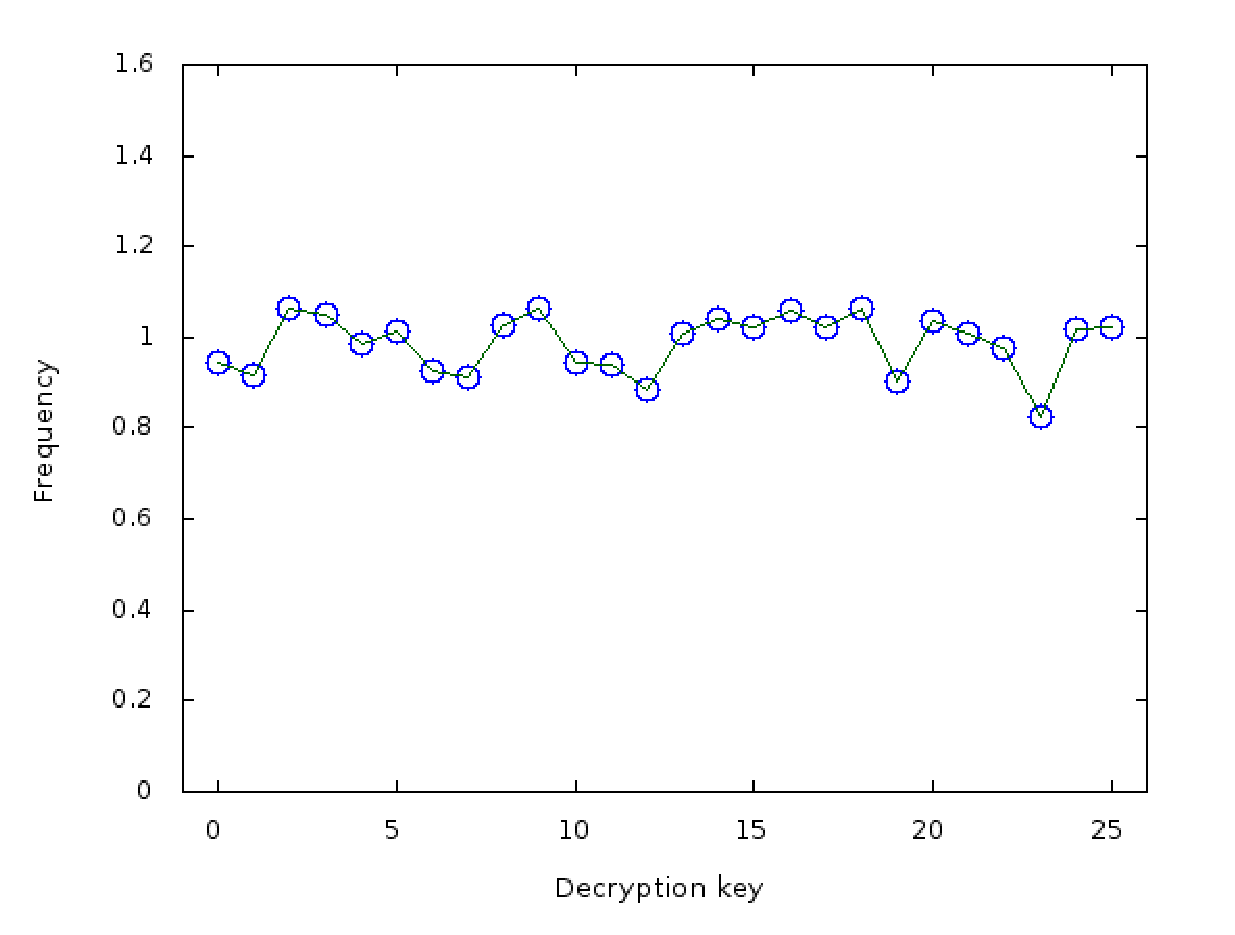
\includegraphics[width=12cm]{seadk_hamhip.eps}
 \caption{Galat kuadrat untuk semua kunci dekripsi pada huruf di posisi yang
          kongruen dengan $1\pmod{5}$ dalam {\it Hamlet} yang dienkripsi
          menggunakan Vigen\`ere dengan kunci
          {\tt hippopotomonstrosesquipedaliophobia}}
 \label{fig:seadk_hamhip}
\end{figure}
Nilai minimum jelas terdapat pada kunci dekripsi 23, tetapi tidak jauh lebih
kecil daripada kemungkinan lain. Selain itu, semua galatnya sekitar sepuluh
kali lebih besar daripada yang tampak pada grafik sebelumnya, seperti
Gambar~\ref{fig:seadk_Cct}.

Jadi, berikut adalah pendekatan kriptanalisis Vigen\`ere. Coba semua panjang
kunci $\ell$ hingga suatu batas $L$. Batas ini ditentukan oleh waktu komputasi
yang tersedia dan tidak boleh begitu besar sehingga pengambilan huruf-huruf
berselang $\ell$ posisi dari cipherteks menyisakan terlalu sedikit huruf untuk
analisis frekuensi yang wajar. Untuk setiap $\ell$ anak untaian yang terdiri
atas huruf-huruf berselang $\ell$ posisi dan masing-masing dimulai pada posisi
$1,\dots,\ell$, terapkan pemecah Caesar. Hasilnya adalah kunci Vigen\`ere optimal
$\vec{k}_\ell=(k_{\ell,1},\dots,k_{\ell,\ell})$ sepanjang $\ell$. Kemudian,
untuk setiap $\ell=1,\dots,L$ dan kunci $\vec{k}_\ell$ yang bersesuaian, hitung
jarak galat kuadrat $d_\ell$ antara cipherteks yang didekripsi menggunakan
$\vec{k}_\ell$ dan distribusi huruf bahasa Inggris baku. Laporkan $\ell$ dan
$\vec{k}_\ell$ sebagai panjang kunci dan kunci Vigen\`ere jika $d_\ell$
merupakan galat kuadrat terkecil yang diperoleh.
\end{discussion}

\ifdefined\suppressallexercises
  {}
\else
  \vfill
  \pagebreak
  \subsection*{Latihan untuk \S\ref{sec:FSiCFA}}
\fi

\begin{exercise}\label{exer:twocaesardecrypts}
Dapatkah Anda menemukan cipherteks Caesar yang memiliki dua hasil dekripsi yang
keduanya tampak seperti bahasa Inggris yang wajar selama serangan brute force?
Jika dapat, berikan contoh yang tepat beserta kunci dekripsinya.
\end{exercise}

\begin{exercise}
Apakah latihan sebelumnya (\ref{exer:twocaesardecrypts}) menjadi lebih sulit
atau lebih mudah untuk cipher Vigen\`ere? Berikan alasan dan contoh.
\end{exercise}

\begin{exercise}
Dalam merancang kriptosistem yang aman, enkripsi yang lebih banyak tampaknya
lebih baik. Jadi, bagaimana jika kita mengenkripsi teks terang dengan satu
kriptosistem, lalu mengenkripsi kembali cipherteks yang dihasilkan untuk membuat
sebuah cipherteks super?

Sejauh ini kita mempunyai dua kriptosistem berkunci pendek: Caesar dan
Vigen\`ere. Kita juga mempunyai pad sekali pakai, tetapi sistem itu sudah aman
secara sempurna dan mempunyai kunci besar, yaitu pad-pad tersebut, sehingga
tidak akan kita pertimbangkan. Andaikan saya membuat kriptosistem baru yang
menerapkan suatu kombinasi enkripsi Caesar dan Vigen\`ere secara berurutan,
semuanya dengan kunci berbeda. Apakah hasilnya merupakan kriptosistem yang jauh
lebih aman? Mengapa atau mengapa tidak?
\end{exercise}

\vfill
\pagebreak
\ifdefined\boundaryeighteen
  \def\finishboundaryeighteen{\backmatter
    \bibliographystyle{amsalpha}
    \bibliography{refs}
    \printindex
    \end{document}}
\else
  \let\finishboundaryeighteen\relax
\fi
\finishboundaryeighteen
\section{Kripto Kunci Publik: Kriptosistem RSA}
\label{sec:tRSAC}

\begin{discussion}
Andaikan Alice dan Bob tidak pernah berkesempatan bertemu langsung, tetapi tetap
ingin bertukar pesan yang dirahasiakan dari Eve. Apa yang dapat mereka lakukan?

Hal ini tampak mustahil dalam konteks kriptosistem yang telah kita bahas.
Mari kita uraikan bagian penting yang membuatnya begitu sulit.
\end{discussion}
\begin{definition}\label{def:symmetric cipher}
\index{cipher/kriptosistem/enkripsi simetris}
Sebuah {\bf cipher simetris} (atau {\bf kriptosistem simetris}) terdiri atas
bagian-bagian berikut, yang semuanya diketahui oleh kedua pihak yang
berkomunikasi dan juga oleh masyarakat umum:
\begin{itemize}
\item ruang pesan $\Mm$;
\item ruang kunci $\Kk$;
\item algoritme enkripsi yang menghasilkan cipherteks $c=e_k(m)$ untuk setiap
pilihan $k\in\Kk$ dan $m\in\Mm$;
\item algoritme dekripsi yang, jika diberi cipherteks $c$ dan $k\in\Kk$,
menghasilkan pesan $d_k(c)\in\Mm$ serta memenuhi
$d_k(e_k(m))=m\ \forall k\in\Kk,m\in\Mm$.
\end{itemize}
Alice dan Bob dapat menggunakan cipher simetris semacam ini dengan menyepakati
secara privat sebuah kunci $k\in\Kk$ yang akan dipakai untuk enkripsi dan
dekripsi. Karena itu, kriptosistem simetris juga disebut
{\bf kriptosistem kunci privat}.
\end{definition}

\begin{discussion}
Secara grafis:
\end{discussion}
\vskip4mm
\begin{center}
\begin{tabular}{|c|c|c|}
\multicolumn{3}{l}{\bf\ \ \ Penyiapan dan notasi dasar kripto kunci privat:}\\
\hline
\multicolumn{3}{|c|}{komunikasi privat}\\
\multicolumn{3}{|c|}{Alice\quad$\longleftrightarrow$\quad pertukaran kunci bersama
$k\in\Kk$\quad$\longleftrightarrow$\quad Bob}\\
\hline
\hline
 & pada jaringan publik & \\
\hline
\ pesan $m_A\in\Mm$\  & & \\
\ \ hitung $c_A=e_k(m_A)$\ \ &  & \\
kirim $c_A$ &\ \quad$\rightarrowtail\ \ \ $ cipherteks\ $c_A\ \ \ \rightarrowtail$\quad\ & terima $c_A$\\
& & hitung $m_A=d_k(c_A)$\\
\hline
& & pesan $m_B\in\Mm$ \\
& &\ \ hitung $c_B=e_k(m_B)$\ \ \\
terima $c_B$ &\ \quad$\leftarrowtail\ \ \ $ cipherteks\ $c_B\ \ \ \leftarrowtail$\quad\ & kirim $c_B$ \\
hitung $m_B=d_k(c_B)$ & & \\
\hline
\multicolumn{3}{|l|}{\quad\qquad\qquad\qquad\qquad$\vphantom{\begin{matrix}1\\1\end{matrix}}${\it dan seterusnya}} \\
\hline
\end{tabular}
\end{center}
\begin{discussion}

\ \vskip2mm\ 
Demi keamanan kriptosistem di atas, ruang kunci $\Kk$ harus cukup besar, atau
keseluruhan sistem harus disusun sedemikian rupa sehingga sulit menentukan
apakah suatu kemungkinan dekripsi tertentu sah (atau keduanya). Jika tidak,
Eve dapat melakukan serangan brute force dengan mencoba semua kemungkinan kunci
$k\in\Kk$ dan melihat hasil $d_k(c)$ mana yang masuk akal sebagai dekripsi.

Bagaimanapun, karena memerlukan pertukaran kunci privat di awal, kriptosistem
simetris tidak cocok untuk situasi yang diajukan pada awal bagian ini. Kita
memerlukan jenis kriptosistem yang berbeda.
\end{discussion}
\begin{definition}\label{def:asymmetric cipher}
\index{cipher/kriptosistem/enkripsi asimetris}
Sebuah {\bf cipher asimetris} (atau {\bf kriptosistem asimetris}) terdiri atas
bagian-bagian berikut, yang semuanya diketahui oleh setiap pihak yang
berkepentingan, baik yang sah maupun yang tidak:
\begin{itemize}
\item ruang pesan $\Mm$;
\item ruang kunci enkripsi $\Kk_e$;
\item ruang kunci dekripsi $\Kk_d$;
\item algoritme pembangkitan kunci $\mathsf{Gen}$ yang menghasilkan pasangan
terkait $(k_e,k_d)\in\Kk_e\times\Kk_d$;
\item algoritme enkripsi yang menghasilkan cipherteks $c=e_{k_e}(m)$ untuk
setiap pilihan $k_e\in\Kk_e$ dan $m\in\Mm$;
\item algoritme dekripsi yang, jika diberi cipherteks $c$ dan
$k_d\in\Kk_d$, menghasilkan pesan $d_{k_d}(c)\in\Mm$ serta, untuk setiap
pasangan $(k_e,k_d)$ yang dihasilkan $\mathsf{Gen}$, memenuhi
$d_{k_d}(e_{k_e}(m))=m\ \forall m\in\Mm$.
\end{itemize}
Untuk menggunakan kriptosistem semacam ini, Bob menjalankan $\mathsf{Gen}$ untuk
memperoleh pasangan $(k_e,k_d)$. Ia merahasiakan kunci dekripsi $k_d$, tetapi
menyediakan kunci enkripsi $k_e$ kepada publik (mungkin melalui situs webnya).
Karena itu, $k_e$ disebut {\bf kunci publik} milik Bob dan $k_d$ disebut
{\bf kunci privat} milik Bob, sedangkan keseluruhan sistem disebut
{\bf kriptosistem kunci publik}.\index{kriptosistem kunci publik}
\index{kunci publik}\index{kunci privat}
\end{definition}

\begin{discussion}
Secara grafis:
\end{discussion}
\vskip4mm
\begin{center}
\begin{tabular}{|c|c|c|}
\multicolumn{3}{l}{\bf\ \ \ Penyiapan dan notasi dasar kripto kunci publik:}\\
\hline
Alice & pada jaringan publik & Bob\\
\hline
& & jalankan $\mathsf{Gen}$ untuk memperoleh\\
& & $(k_e,k_d)\in\Kk_e\times\Kk_d$\\
unduh $k_e$ &\ \quad$\leftarrowtail\ \ \ $ kunci publik\ $k_e\ \ \ \leftarrowtail$\quad\  & terbitkan $k_e$\\
\hline
pesan $m\in\Mm$  & & \\
\ \ hitung $c=e_{k_e}(m)$\ \ &  & \\
kirim $c$ &\ \quad$\rightarrowtail\ \ \ $ cipherteks\ $c\ \ \ \rightarrowtail$\quad\ & terima $c$\\
& & hitung $m=d_{k_d}(c)$\\
\hline
\end{tabular}
\end{center}
\begin{discussion}

\ \vskip2mm\ 
Seperti sebelumnya, keamanan kriptosistem ini terhadap serangan brute force
bergantung pada ukuran $\Kk_d$. Selain itu, karena kunci dan algoritme enkripsi
diketahui Eve, ruang pesan $\Mm$ tidak boleh terlalu kecil. Jika $\Mm$ kecil,
Eve cukup menghitung semua enkripsi $e_{k_e}(m)$ untuk setiap $m\in\Mm$, lalu
membandingkannya dengan cipherteks $c$ yang berhasil dicegatnya.

Serangan terhadap ruang pesan ini dapat dicegah dengan memperbesar ruang
tersebut secara artifisial. Biasanya, orang menambahkan data berikut.
\end{discussion}
\begin{definition}
{\bf Salt kriptografis} adalah data acak yang ditambahkan pada pesan yang hendak
dikirim Alice kepada Bob sebelum dienkripsi, lalu dihapus secara otomatis di
sisi Bob.
\end{definition}
\begin{discussion}
Setelah Alice menambahkan salt pada pesannya, Eve harus menelusuri seluruh ruang
pesan beserta salt, yang dapat jauh lebih besar daripada $\Mm$.

Sebagai manfaat tambahan, salt membuat cipherteks hampir selalu berbeda pada
setiap pengiriman rahasia, sekalipun plainteksnya sama, apabila dipilih secara
independen dari ruang yang cukup besar. Eve tentu mengetahui bahwa Alice dan Bob
sedang berkomunikasi, tetapi dengan hanya membandingkan kesamaan cipherteks,
analisisnya tidak lagi dapat mengenali pengiriman ulang pesan yang sama secara
andal. Tanpa salt, Eve yang
cermat mungkin dapat menghubungkan cipherteks pesan dengan tindakan di dunia
nyata, sehingga pada dasarnya mengetahui hasil dekripsinya tanpa memecahkan
kriptosistem. Jika salt dipilih secara independen dari ruang yang cukup besar,
korelasi yang hanya mengandalkan kesamaan cipherteks menjadi sangat tidak andal,
sebab peluang penggunaan ulang salt yang sama menjadi sangat kecil.

Karena kunci enkripsi Bob $k_e$ tersedia bagi publik, seluruh keamanan
kriptosistem ini runtuh jika Eve dapat memulihkan kunci privat $k_d$ yang
bersesuaian. Di sisi lain, Bob harus dapat membangkitkan pasangan $(k_e,k_d)$
secara layak pada tahap penyiapan. Asimetri antara komputasi maju yang mudah dan
pemulihan rahasia yang sulit ini biasanya dibangun dari fungsi dengan sifat
khusus berikut.
\end{discussion}
\begin{definition}\label{def:onewayfcn}\index{fungsi satu arah}
Fungsi injektif $f:A\to B$ yang dapat dihitung dalam waktu wajar pada komputer
standar (klasik), tetapi inversnya tidak dapat dihitung secara layak, disebut
{\bf fungsi satu arah} [atau {\bf fungsi satu arah kriptografis}].
\end{definition}
\begin{discussion}

\ \vskip1mm

Perkalian dua bilangan, bahkan dua bilangan yang sangat besar, dapat dilakukan
komputer dengan cukup cepat. Menentukan apakah bilangan yang sangat besar itu
prima atau komposit juga ternyata sangat cepat (lihat
\cite{agrawal2004primes} untuk hasil mengagumkan dalam sejarah panjang uji
keprimaan ini).

Namun, belum ditemukan cara klasik yang layak untuk {\it memfaktorkan}
semiprima RSA yang cukup besar, yaitu hasil kali dua prima besar berukuran
sebanding.\footnote{Pernyataan ini berlaku untuk komputer {\it klasik}.
Terdapat algoritme pemfaktoran yang efisien pada {\it komputer kuantum}
\index{komputer kuantum}; lihat \cite{shor1994algorithms} dan
\cite{nielsen2010quantum}.} Pembatasan bentuk ini penting: bilangan genap atau
bilangan dengan faktor kecil dapat difaktorkan dengan mudah, berapa pun
besarnya. Sebagai contoh, salah satu semiprima RSA terbesar yang pernah
difaktorkan pada saat naskah sumber ditulis adalah soal tantangan terkenal
{\bf RSA-768}, sebuah bilangan komposit 232 digit (768 bit). Bilangan itu
akhirnya difaktorkan pada 2009 setelah jaringan berisi ratusan komputer bekerja
bersama selama sekitar dua tahun, meskipun tidak secara eksklusif mengerjakan
soal tersebut. Semiprima RSA sejenis yang lebih besar mudah dibuat, tetapi pada
umumnya jauh lebih sulit difaktorkan.

Karena itu, fungsi yang mengalikan dua bilangan prima besar berukuran sebanding
untuk menghasilkan semiprima yang sangat besar merupakan calon fungsi satu
arah kriptografis yang baik.

Pada 1978, Ron Rivest,\index{Rivest, Ron} Adi Shamir\index{Shamir, Adi}, dan
Leonard Adleman\index{Adleman, Leonard} menjelaskan
(\cite{rivest1978method}) kriptosistem kunci publik berikut yang didasarkan pada
fungsi satu arah tersebut.
\end{discussion}
\begin{definition}\label{def:rsacryptosystem}
\index{RSA!kriptosistem}
Bob memulai dengan memilih dua bilangan prima sangat besar yang berbeda, $p$
dan $q$. Hasil kalinya $n=pq$ disebut {\bf modulus RSA} yang bersesuaian.
\index{RSA!modulus} Bob juga memilih bilangan $e$ yang memenuhi
$1<e<\phi(n)$ dan $\gcd(e,\phi(n))=1$.
\index{fungsi $\phi$/totient Euler!digunakan}
\index{pembagi persekutuan terbesar!digunakan} Bilangan $e$ biasanya memiliki
sangat sedikit angka 1 ketika ditulis dalam basis dua, misalnya $3$ atau
$65537=10000000000000001_2$. Bilangan ini disebut {\bf eksponen RSA}.
\index{RSA!eksponen}

{\bf Kunci publik} [{\bf enkripsi}] {\bf RSA} $k_e$ terdiri atas pasangan
$(n,e)$; himpunan semua pasangan semacam itu adalah $\Kk_e$.

{\bf Kunci privat} [{\bf dekripsi}] {\bf RSA} $k_d$ terdiri atas pasangan
$(n,d)$, dengan $d$ dipilih sebagai wakil positif terkecil dari
\index{fungsi $\phi$/totient Euler!digunakan}
$$
d=e^{-1}\pmod{\phi(n)},
$$
dan $\Kk_d$ adalah himpunan semua pasangan semacam itu.

Algoritme pembangkitan kunci RSA $\mathsf{Gen}$ memilih $p,q,e$ seperti di atas,
menghitung $n=pq$ dan $d=e^{-1}\pmod{\phi(n)}$, lalu menghasilkan pasangan
$(k_e,k_d)=((n,e),(n,d))$. Data faktor $p,q$ (atau $\phi(n)$) digunakan pada
tahap penyiapan dan tidak perlu menjadi bagian kunci dekripsi operasional.

Ruang pesan kriptosistem ini adalah
$\Mm=\left\{m\in\ZZ \mid 0\le m<n\right\}$.

Enkripsi diberikan oleh
$$
c=e_{(n,e)}(m)=m^e\pmod{n}\ .
$$

Dekripsi diberikan oleh
$$
d_{(n,d)}(c)=c^d\pmod{n}\ .
$$

Keseluruhan sistem di atas disebut {\bf kriptosistem RSA}.
\end{definition}

\begin{discussion}
Secara grafis:
\end{discussion}
\vskip4mm
\begin{center}
\begin{tabular}{|c|c|c|}
\multicolumn{3}{l}{\bf\ \ \ Penyiapan dan notasi kriptosistem RSA:}\\
\hline
Alice & pada jaringan publik & Bob\\
\hline
& & pilih prima besar berbeda $p$ dan $q$\\
& & hitung {\bf modulus RSA} $n=pq$\\
& & pilih {\bf eksponen RSA} $e\in\NN$\\
& & dengan $1<e<\phi(n)$\\
& & dan $\gcd(e,\phi(n))=1$\\
unduh $k_e$ &\ \quad$\leftarrowtail\ \ \ $ kunci publik\ $k_e\ \ \ \leftarrowtail$\quad\  & terbitkan $k_e=(n,e)$\\
& & hitung $d=e^{-1}\pmod*{\phi(n)}$\\
\hline
pesan $m\in\Mm$  & & \\
hitung $c=e_{(n,e)}(m)$& & \\
${}=m^e\pmod*{n}$\ \ &  & \\
kirim $c$ &\ \quad$\rightarrowtail\ \ \ $ cipherteks\ $c\ \ \ \rightarrowtail$\quad\ & terima $c$\\
& & hitung $m=d_{(n,d)}(c)$\\
& & ${}=c^d\pmod*{n}$\\
\hline
\end{tabular}
\end{center}
\begin{discussion}

\ \vskip2mm\ 
Pertama-tama, kita perlu memastikan bahwa sistem ini memenuhi syarat dasar agar
berfungsi sebagai kriptosistem.
\end{discussion}
\begin{proposition}\label{prop:RSAworks}
Gunakan notasi dalam definisi kriptosistem RSA di atas. Untuk setiap pesan
$m\in\Mm$, berlaku $d_{(n,d)}(e_{(n,e)}(m))=m$.
\end{proposition}
\begin{proof}
Setiap $m\in\Mm$ mewakili suatu kelas dalam $\ZZ/n\ZZ$. Kita tidak akan
membedakan kelas tersebut dari wakilnya $m$ yang memenuhi $0\le m<n$.

Kita membentuk $d$ sebagai $d=e^{-1}\pmod{\phi(n)}$.
\index{fungsi $\phi$/totient Euler!digunakan} Artinya,
$e\cdot d\equiv1\pmod{\phi(n)}$, sehingga terdapat $k\in\ZZ$ dengan
$e\cdot d=1+k\phi(n)$.

Kemudian, menurut Teorema Euler~\ref{thm:eulers}
\index{Teorema Euler!digunakan}, untuk setiap $m\in\Mm$ yang memenuhi
$\gcd(m,n)=1$ \index{pembagi persekutuan terbesar!digunakan}
\index{fungsi $\phi$/totient Euler!digunakan}, berlaku
$$
d_{(n,d)}(e_{(n,e)}(m))\equiv(m^e)^d=m^{ed}=m^{1+k\phi(n)}\equiv m\cdot(m^{\phi(n)})^k\equiv m\cdot(1)^k\equiv m\pmod{n}
$$
seperti yang diinginkan. Kasus $\gcd(m,n)\neq1$
\index{pembagi persekutuan terbesar!digunakan} menjadi
Latihan~\ref{exc:RSAmessagecommonfactor} dalam bagian ini.
\end{proof}
\begin{discussion}

Selain memastikan fungsi dasarnya, kita perlu menilai seberapa praktis RSA.
Mari kita telusuri dengan cermat algoritme yang diperlukan pada setiap langkah.

\end{discussion}
\begin{enumerate}
\begin{discussion}
\item Bob harus memilih prima besar $p$ dan $q$. Seperti telah disebutkan,
terdapat algoritme yang dapat menentukan keprimaan suatu bilangan dalam waktu
wajar. Lebih tepatnya, komputer (klasik) dapat menentukan apakah bilangan $k$
prima dalam waktu yang dibatasi oleh suatu fungsi polinomial dari $\log(k)$.
[Inilah arti lazim {\it komputasi layak}\index{komputasi layak!definisi} dalam
kriptologi.]
\item Selain itu, jumlah prima cukup banyak sehingga Eve tidak dapat melakukan
pencarian brute force atas semua kemungkinan. Hal ini mengikuti Teorema Bilangan
Prima, yang memberikan banyaknya prima secara asimtotik.
\end{discussion}
\begin{theorem}\label{thm:primenumber}\index{Teorema Bilangan Prima}
Untuk $x\in\RR$ dengan $x>0$, definisikan {\bf fungsi penghitung prima}
\index{fungsi penghitung prima} sebagai
$\pi(x)=\#\{p\in\NN\mid p\text{ prima dan }p\le x\}$. Maka
$$
\lim_{x\to\infty} \frac{\pi(x)}{x/\ln(x)} = 1.
$$
\end{theorem}
\begin{discussion}
Teorema ini merupakan salah satu permata teori bilangan analitik. Teorema ini
dibuktikan pada 1896 oleh Jacques Hadamard dan Charles Jean de la
Vall\'ee-Poussin, walaupun bagian-bagian pentingnya telah diketahui sebelumnya
oleh tokoh seperti Euler, Legendre, dan Riemann. Buktinya sulit, bahkan bukti
{\it elementer} yang diberikan Atle Selberg dan Paul Erd\"os pada 1948.

Salah satu akibat Teorema Bilangan Prima ialah bahwa peluang sebuah bilangan $k$
yang dipilih secara acak adalah prima kira-kira $1/{\ln(k)}$. Sebagai
contoh, untuk mencari prima 200 digit, kita memilih bilangan acak berukuran itu
dan perlu menguji sekitar $\ln(10^{200})=461$ bilangan sebelum memperoleh suatu
prima. Jumlah komputasi ini masih wajar.
\item Setelah memiliki modulus RSA $n=pq$, kita dapat menghitung fungsi totient
Euler $\phi(n)=(p-1)(q-1)$\index{fungsi $\phi$/totient Euler!digunakan}
\index{fungsi $\phi$/totient Euler!nilai} hampir seketika dengan
Teorema~\ref{thm:phiismultiplicative}.
\item Menentukan eksponen RSA $e$ yang relatif prima terhadap $\phi(n)$
\index{fungsi $\phi$/totient Euler!digunakan} tidak sulit karena terdapat banyak
pilihan. Bahkan, dalam arti yang tepat, peluang bahwa dua bilangan yang dipilih
secara acak saling relatif prima adalah $\frac{6}{\pi^2}$ (untuk
pernyataan tepat beserta buktinya, lihat \cite{hardy1979introduction}).
Pengujian calon $e$ juga efisien sebab, seperti akan kita lihat dalam
Latihan~\ref{exc:EAcomplexitybound}, waktu Algoritma Euklides
\index{Algoritma Euklides!digunakan} dibatasi oleh fungsi polinomial dari
logaritma bilangan-bilangan yang terlibat. Jadi, komputasinya
{\it layak}\index{komputasi layak!digunakan}.
\item Selanjutnya, $d=e^{-1}\pmod{\phi(n)}$ dapat dihitung sangat cepat dengan
Algoritma Euklides diperluas\index{fungsi $\phi$/totient Euler!digunakan}
(Teorema~\ref{thm:euclideanalg})\index{Algoritma Euklides!digunakan}. Algoritme
ini tentu lebih lambat daripada Algoritma Euklides dasar, tetapi tetap layak.
\index{komputasi layak!digunakan}
\item Enkripsi dan dekripsi RSA sama-sama berupa pemangkatan suatu bilangan
modulo $n$. Untungnya, terdapat algoritme bernama {\bf eksponensiasi modular
cepat}\index{eksponensiasi modular cepat} yang juga menyelesaikannya dalam waktu
yang dibatasi oleh fungsi polinomial dari logaritma bilangan-bilangan yang
diberikan.
\item Persoalan praktis terakhir ialah cara Alice benar-benar menggunakan RSA
untuk mengirim pesan yang diinginkannya, bukan sekadar bilangan $m\in\ZZ$ yang
memenuhi $0\le m<n$.

Ini merupakan persoalan baku dalam kriptografi matematis dan mempunyai solusi
baku. Biasanya, Alice harus mengambil pesannya karakter demi karakter lalu
menyalinnya menjadi barisan bilangan menurut suatu standar yang diterima. Sejak
dekade 1960-an, hal ini dilakukan menggunakan {\bf kode ASCII} [American Standard Code
for Information Interchange, Kode Standar Amerika untuk Pertukaran Informasi]
\index{ASCII}. ASCII memberikan bilangan biner 7 bit untuk 26 huruf alfabet
Latin (modern), baik huruf besar maupun kecil, serta untuk sekumpulan simbol
yang lazim dan beberapa tambahan modern yang biasanya tidak dicetak, seperti
$11110_2$ {\it Pemisah Rekaman}, $111_2$ {\it Bel}, dan $1011_2$ {\it Tab
Vertikal}. Kini, kode-kode ASCII selalu disimpan dalam satu byte (8 bit) dengan
menambahkan bit $0$ di depan.

Ketika World Wide Web menjadi fenomena global, kebutuhan akan lebih banyak
alfabet dan bahkan sistem tulisan nonalfabetis (seperti aksara Tionghoa) terus
meningkat. Hal ini menghasilkan sistem bernama {\bf Unicode}\index{Unicode}
yang, pada versi 6.3 tahun 2013, memuat lebih dari 110.000 karakter. Unicode
disimpan dengan berbagai pengodean. Dua yang paling umum adalah {\bf UTF-8},
yang menggunakan satu hingga empat byte per karakter, dan {\bf UTF-16}, yang
menggunakan dua atau empat byte per karakter.

Jadi, Alice biasanya menuliskan pesannya dalam ASCII atau Unicode, menyambungkan
semua byte secara berurutan, lalu memotong seluruh pesan menjadi blok-blok
sepanjang $b$ bit. Di sini $b\in\NN$ dipilih sebagai nilai terbesar yang
memenuhi $2^b<n$. Dengan demikian, setiap blok $b$ bit dapat dipandang sebagai
bilangan bulat $m\in\ZZ$ yang memenuhi $0\le m<n$, sehingga RSA dapat diterapkan
pada pesan tersebut satu blok demi satu blok.

(Kita mengabaikan banyak perincian, misalnya cara menyisakan ruang untuk salt,
pendekatan lain, dan persoalan struktur blok. Lihat referensi baku tentang
kriptografi, seperti \cite{ferguson2003practical} atau
\cite{menezes1996handbook}.)
\end{discussion}
\end{enumerate}

\ifdefined\suppressallexercises
  {}
\else
  \vfill
  \pagebreak
  \subsection*{Latihan untuk \S\ref{sec:tRSAC}}
\fi

\begin{exercise}\label{exc:RSAmessagecommonfactor}
Dalam soal ini, Anda akan menyelesaikan bukti
Proposisi~\ref{prop:RSAworks}, yang menyatakan bahwa dekripsi RSA berfungsi
dengan benar dalam semua kasus.

Sebagai langkah pertama, nyatakan secara formal dan buktikan sebuah lema:
untuk prima berbeda $p$ dan $q$, dua bilangan bulat $r$ dan $s$ kongruen modulo
$pq$ jika dan hanya jika keduanya kongruen modulo $p$ dan modulo $q$.
{\it [Petunjuk: Teorema Sisa Cina.]}\index{Teorema Sisa Cina}

Sekarang, gunakan hasil di atas untuk membuktikan kasus yang belum dibuktikan
dalam Proposisi~\ref{prop:RSAworks}. Diberikan prima berbeda $p$ dan $q$,
tetapkan $n=pq$. Misalkan $e\in\NN$ memenuhi $\gcd(e,\phi(n))=1$
\index{pembagi persekutuan terbesar!digunakan} dan $d\in\NN$ merupakan invers
$e$ modulo $\phi(n)$.\index{fungsi $\phi$/totient Euler!digunakan} Buktikan
bahwa untuk setiap $m\in\ZZ$ yang memenuhi $0\le m<n$ dan
$\gcd(m,n)\neq1$, berlaku
$m^{ed}\equiv m\pmod{n}$.
\end{exercise}

\begin{exercise}
Berapa banyak komputasi yang diperlukan untuk menghitung $a^k\pmod{n}$ bagi
$a\in\ZZ$ dan $k,n\in\NN$ dengan $n\ge2$?

Misalkan $D$ adalah panjang maksimum masukan $a$, $k$, dan $n$, diukur dalam
digit. Perkalian dua bilangan merupakan instruksi dasar pada sebagian besar
komputer modern dan dapat dianggap memerlukan satu satuan waktu. (Atau, Anda
dapat melakukan sejumlah manipulasi lebih kecil yang banyaknya dibatasi oleh
fungsi polinomial dari panjang operan; pilihan ini tidak memengaruhi bagian
selanjutnya dari soal.) Demikian pula, pembagian bersisa merupakan satu
instruksi mesin (misalnya pada prosesor keluarga Pentium) atau dapat dilakukan
dengan cara sekolah dasar dalam waktu polinomial terhadap panjang masukannya.

Anggaplah pekerjaan untuk melakukan satu perkalian lalu mereduksi modulo $n$
dibatasi oleh fungsi polinomial $p(D)$.

Jika kita sekadar membentuk $k$ faktor $a$, melakukan $k-1$ perkalian, dan
mereduksi modulo $n$ pada setiap langkah, waktunya berorde $O(kp(D))$. Karena
bilangan $k$ yang terdiri atas $D$ digit dapat berorde $10^D$, batas waktu ini
bersifat {\it eksponensial} terhadap panjang masukan $D$.

Cobalah menemukan algoritme eksponensiasi yang jauh lebih cepat, dengan waktu
polinomial alih-alih eksponensial.

{\it [Petunjuk: (1) Buat tabel kuadrat berulang dari $a$ modulo $n$, yaitu
$a^2$, $a^4$, $a^8$, dan seterusnya. (2) Tuliskan $k$ dalam basis dua dan
uraikan $a^k$ menggunakan bentuk biner $k$, aturan pemangkatan biasa, dan tabel
tersebut. Hasil akhirnya harus mendeskripsikan cara menghitung
$a^k\pmod{n}$; periksa dengan cermat berapa banyak waktu yang diperlukan.]}
\end{exercise}

\begin{exercise}\label{exc:EAcomplexitybound}
Untuk $k\in\NN$, lakukan permainan berikut:
\begin{enumerate}
\item gunakan Algoritma Pembagian\index{Algoritma Pembagian!digunakan} untuk
membagi $k$ dengan dua dan memperoleh hasil bagi $q$ serta sisa $r$;
\item ganti $k\leftarrow q$;
\item jika $k>0$, ulangi dari langkah (1); jika tidak, berhenti.
\end{enumerate}
Berikan batas banyaknya langkah sampai permainan ini berhenti. Nyatakan jawaban
sebagai fungsi dari $k$, fungsi dari banyaknya bit yang diperlukan untuk
menuliskan $k$ dalam basis dua, atau fungsi dari banyaknya digit yang diperlukan
untuk menuliskan $k$ dalam basis 10.

Tunjukkan bahwa setiap dua langkah Algoritma Euklides membuat suku-suku sisa
$r_i$ berkurang sekurang-kurangnya dengan faktor $1/2$. Dengan kata lain, jika
kita menggunakan notasi Teorema~\ref{thm:euclideanalg}, maka
$r_{j+2}<\frac12r_j$ untuk setiap $j\in\ZZ$ yang memenuhi $j\ge0$.

Jelaskan mengapa hal ini berarti Algoritma Euklides
\index{Algoritma Euklides!digunakan} memerlukan paling banyak
$2\lfloor\log_2(b)\rfloor+1$ langkah pembagian untuk menghitung $\gcd(a,b)$
\index{pembagi persekutuan terbesar!digunakan}. Turunkan pula batas linear
sebesar paling banyak tujuh kali banyaknya digit desimal $b$, dengan memeriksa
kasus ujung kecil secara terpisah.
{\it [Petunjuk: berapakah $\log_2(10)$?]}

Jelaskan mengapa hasil ini berarti Algoritma Euklides
\index{Algoritma Euklides!digunakan} merupakan komputasi yang {\it layak}
secara kriptologis\index{komputasi layak!digunakan}, dalam pengertian bagian
ini.
\end{exercise}

\vfill
\pagebreak
\ifdefined\boundarynineteen
  \def\finishboundarynineteen{\backmatter
    \bibliographystyle{amsalpha}
    \bibliography{refs}
    \printindex
    \end{document}}
\else
  \let\finishboundarynineteen\relax
\fi
\finishboundarynineteen
\section{Tanda Tangan Digital}
\label{sec:DSs}

\begin{discussion}
Kriptosistem kunci publik memungkinkan beberapa penggunaan yang tidak tersedia
pada kriptosistem simetris. Salah satu penggunaan yang makin penting dalam
ekonomi digital modern ialah pembuatan {\it tanda tangan digital}: bagian dari
dokumen elektronik yang diharapkan memiliki salah satu sifat tanda tangan
fisik, yakni sulit dipalsukan oleh penyamar. Dokumen bertanda tangan semacam itu
mungkin diperlukan, misalnya, jika Bob dari bagian sebelumnya (yang memasang
kunci publik RSA-nya di situs web) hendak mengirim kontrak yang mengikat secara
hukum melalui surel. Barangkali Alice dan Bob ingin mengirim kepada calon
pemilik rumah mereka, Larry, perjanjian sewa bertanda tangan untuk apartemen
yang akan mereka tinggali bersama. Ketika menerima surel dari Bob yang berbunyi
``Saya setuju terikat oleh ketentuan perjanjian sewa ini,'' Larry perlu yakin
bahwa surel tersebut benar-benar berasal dari Bob; tanda tangan digital dapat
memberikan keyakinan itu.

Untuk skema dasar berikut, kita memerlukan sifat tambahan. Setiap pesan yang
hendak ditandatangani harus berada dalam domain operasi privat $d_{k_d}$; untuk
setiap pasangan $(k_e,k_d)$ yang dihasilkan $\mathsf{Gen}$ dan setiap $m\in\Mm$,
harus berlaku $e_{k_e}(d_{k_d}(m))=m$, seperti pada RSA. Definisi umum
kriptosistem asimetris sebelumnya hanya mensyaratkan urutan sebaliknya.

Bob lalu dapat melakukan hal berikut. Ia mengambil salinan perjanjian sewa,
menambahkan bagian di akhir yang menyatakan persetujuannya atas ketentuan
tersebut dan memuat informasi pengenal pribadi (mungkin pindaian surat izin
mengemudinya). Sebut seluruh bongkah data ini $m$. Bob kemudian menerapkan
algoritme {\it dekripsi} dengan kunci privat (dekripsi) $k_d$, sehingga
diperoleh $s=d_{k_d}(m)$. Nilai $s$ ini disebut tanda tangan Bob atas pesan $m$.
Ia lalu mengirimkan $m$ dan $s$ kepada Larry melalui surel.

Ketika menerima pesan bertanda tangan ini, Larry mula-mula memisahkan tanda
tangan $s$, lalu menghitung enkripsinya, $e_{k_e}(s)$, menggunakan kunci publik
yang ia unduh dari situs web Bob. Berdasarkan sifat tambahan di atas, hasilnya
harus sama dengan $m$. Verifikasi $e_{k_e}(s)=m$ itu sendiri hanya menetapkan
konsistensi aljabar pasangan $(m,s)$ terhadap kunci publik tersebut. Untuk
menyimpulkan bahwa Bob menghasilkan tanda tangan dan bahwa pesan tidak berubah
sejak ditandatangani, Larry juga harus mengandalkan skema tanda tangan yang tak
dapat dipalsukan, kunci privat Bob yang tidak terkompromi, serta pengikatan
tepercaya antara identitas Bob dan kunci publik tersebut. Bahkan dengan
asumsi-asumsi itu, verifikasi tidak dengan sendirinya membuktikan identitas
pengirim surel ataupun kebaruan pesan, sebab pasangan bertanda tangan yang lama
dapat diteruskan atau diputar ulang oleh siapa pun.

Secara grafis:
\vskip4mm
\end{discussion}
\begin{center}
\resizebox{\textwidth}{!}{%
\begin{tabular}{|c|c|c|}
\multicolumn{3}{l}{\bf\ \ \ Tanda tangan digital dasar:}\\
\hline
Larry & pada jaringan publik & Bob\\
\hline
& & jalankan $\mathsf{Gen}$ untuk memperoleh\\
& & $(k_e,k_d)\in\Kk_e\times\Kk_d$\\
unduh $k_e$ &\ \quad$\leftarrowtail\ \ \ $ kunci publik\ $k_e\ \ \ \leftarrowtail$\quad\  & terbitkan $k_e$\\
\hline
& & pesan $m\in\Mm$ \\
& & hitung $s=d_{k_d}(m)$ \\
terima $(m,s)$&\ \quad$\leftarrowtail\ \ \ $ pesan bertanda tangan\ $(m,s)\ \ \ \leftarrowtail$\quad\ & kirim $(m,s)$\\
\hline
jika $e_{k_e}(s)=m$\qquad\quad \  & &\\
{\sc terima}\qquad\ & &\\
\ \ jika tidak,\qquad\qquad\quad\ & &\\
\ \ {\sc tolak}\qquad\ & &\\
\hline
\end{tabular}%
}
\end{center}
\begin{discussion}

\ \vskip2mm\ 
Salah satu masalah skema ini ialah ukuran pesan secara efektif menjadi dua kali
lipat. Tanda tangan yang lebih kecil dan efisien dapat dibuat dengan
mendekripsi bukan seluruh $m$, melainkan nilai suatu fungsi $h(m)$. Fungsi $h$
harus menerima pesan berukuran sebarang dan menghasilkan ringkasan data yang
kecil, tetapi tetap bergantung pada setiap bagian masukan $m$. Bagaimanapun,
jika $h(m)$ hanya bergantung pada 100 bit pertama $m$, misalnya, Eve yang
berniat jahat dapat mengubah pesan selama pengiriman tanpa terdeteksi selama ia
tidak mengubah 100 bit pertama pesan tersebut.

Kriptolog mempunyai nama untuk fungsi seperti $h$ ini.
\end{discussion}
\begin{definition}\label{def:cryptohashfcn}\index{fungsi hash kriptografis}
Fungsi $h$ yang menerima string bit berpanjang sebarang dan menghasilkan string
bit berpanjang tetap disebut {\bf fungsi hash kriptografis} jika memenuhi
\begin{description}
\item[kemudahan komputasi] nilai $h(m)$ dapat dihitung secara
layak\index{komputasi layak!digunakan} untuk setiap $m$;
\item[ketahanan praimaji]\index{ketahanan praimaji} jika masukan tantangan $M$
dipilih secara acak menurut distribusi yang ditetapkan dan hanya nilai target
$t=h(M)$ yang diberikan, mencari $m$ sedemikian sehingga $h(m)=t$ tidak layak
dilakukan\index{komputasi layak!digunakan};
\item[ketahanan praimaji kedua]\index{ketahanan praimaji kedua} jika diberikan
masukan tertentu $m_1$, mencari masukan lain $m_2$ sedemikian sehingga
$h(m_2)=h(m_1)$ tidak layak dilakukan\index{komputasi layak!digunakan};
\item[ketahanan tumbukan]\index{ketahanan tumbukan} mencari dua pesan berbeda
$m_1\ne m_2$ sedemikian sehingga $h(m_2)=h(m_1)$ tidak layak dilakukan
\index{komputasi layak!digunakan}.
\end{description}
Kata {\it layak} dan {\it tidak layak}\index{komputasi layak!digunakan} di sini
bermakna sama seperti pada bagian sebelumnya: komputasi tersebut dapat atau
tidak dapat diselesaikan dalam waktu yang dibatasi oleh suatu fungsi polinomial
dari ukuran masukan.
\end{definition}
\begin{discussion}

Perhatikan bahwa karena fungsi hash menerima masukan berpanjang sebarang tetapi
mempunyai ukuran keluaran tetap, pasti terdapat tak hingga banyak tumbukan.

Pembuatan fungsi hash kriptografis sedikit menyerupai seni gelap. Ternyata,
jika suatu calon fungsi hash dibangun dengan struktur yang jelas (biasanya
struktur matematis), terutama bila fungsi itu cepat dihitung, komunitas
kriptologi biasanya menemukan cara untuk menembus salah satu syarat
ketahanannya. Karena itu, algoritme yang digunakan secara luas cenderung berupa
komputasi yang sangat {\it ad hoc}, tampak rumit, dan sejauh ini bertahan
terhadap upaya membalikkan fungsi atau mematahkan sifat ketahanannya.

\end{discussion}
\begin{example}\label{eg:md5} Selama kira-kira satu dasawarsa sejak awal
1990-an, fungsi hash kriptografis yang paling luas digunakan bernama
{\tt md5}\index{md5}. Algoritme ini dikembangkan oleh Ron
Rivest\index{Rivest, Ron} dan diterbitkan pada 1992. Ukuran keluaran {\tt md5}
adalah 128 bit.

Walaupun {\tt md5} telah dicurigai memiliki kelemahan sejak pertengahan
1990-an, serangan nyata baru diterbitkan pada 2004, ketika ditunjukkan bahwa
fungsi ini tidak tahan tumbukan\cite{wang2005break}. Pada saat naskah sumber
ini ditulis, {\tt md5} masih digunakan secara luas untuk memeriksa apakah
transfer data berukuran besar mengalami galat transmisi; dengan kata lain,
fungsi ini tetap berguna untuk menguji kerusakan data yang tidak disengaja.
(Dalam konteks pembuktian integritas data terhadap kerusakan yang tidak
disengaja ini, fungsi hash sering disebut {\bf sidik jari}.\index{sidik jari})
\end{example}

\begin{example}\label{eg:SHA1} Sejak akhir 1990-an hingga tidak lama sebelum
naskah sumber ini ditulis, fungsi hash kriptografis yang paling luas digunakan
dan ditanamkan dalam banyak protokol kriptografis yang diterima luas serta
distandardisasi adalah {\tt SHA-1},\index{SHA-1} dengan ukuran keluaran 160 bit.

{\tt SHA-1} dikembangkan oleh Badan Keamanan Nasional Amerika Serikat (NSA)
\index{Badan Keamanan Nasional, AS [NSA]} melalui proses yang sebagian terbuka,
lalu diadopsi oleh Institut Standar dan Teknologi Nasional Amerika Serikat
(NIST)\index{Institut Standar dan Teknologi Nasional, AS [NIST]} sebagai bagian
dari beberapa Standar Pemrosesan Informasi Federal Amerika Serikat
\index{Standar Pemrosesan Informasi Federal, AS}.

Pada 2004, diterbitkan sejumlah penelitian yang menunjukkan bahwa {\tt SHA-1}
mungkin rentan terhadap jenis serangan tertentu. (Lihat
\cite{poritz2004hash}.) Karena itu, pada 2010 NIST mewajibkan banyak aplikasi
perlindungan data federal Amerika Serikat beralih ke fungsi hash lain.
\end{example}

\begin{example}\label{eg:SHA2} Pada saat naskah sumber ini ditulis, sebagian
besar pengguna dan organisasi yang memerhatikan keamanan merekomendasikan
{\tt SHA-2},\index{SHA-2} biasanya dalam varian ``{\tt SHA-256}''
\index{SHA-256} yang memiliki ukuran keluaran 256 bit. Mengingat pengungkapan
ketika itu mengenai keterlibatan NSA\index{Badan Keamanan Nasional, AS [NSA]}
dalam protokol kriptografis dan pelemahan protokol tersebut, partisipasi NSA
dalam pengembangan {\tt SHA-2} mungkin menimbulkan kekhawatiran.
\end{example}

Untuk menerapkan operasi RSA pada keluaran bit $h(m)$, terlebih dahulu gunakan
enkode tanda tangan yang disepakati untuk memperoleh wakil pesan
$H_n(m)\in\Mm=\{0,\dots,n-1\}$. Skema RSA standar menggunakan enkode dan
padding khusus sebelum menerapkan operasi privat; diagram berikut hanya
menunjukkan alur matematis skematis dan bukan konstruksi yang siap dipakai.

\vskip-3mm
\begin{discussion}
Secara grafis:

\end{discussion}
\begin{center}
\resizebox{\textwidth}{!}{%
\begin{tabular}{|c|c|c|}
\multicolumn{3}{l}{\bf\ \ \ Tanda tangan digital RSA:}\\
\hline
Charlie  & pada jaringan publik &  Bob\\
\hline
& & lakukan penyiapan RSA, buat\\
& & $k_e=(n,e)$ dan $d$\\
unduh $k_e$ &\ \quad$\leftarrowtail$\ \ \ kunci verifikasi $k_e\ \ \ \leftarrowtail$\quad\  & terbitkan $k_e$\\
\hline
& & pesan $m\in\Mm$\\
& & hitung $s=(H_n(m))^d\pmod n$\\
terima $(m,s)$&\ \quad$\leftarrowtail\ \ \ $ pesan bertanda tangan\ $(m,s)\ \ \ \leftarrowtail$\quad\ & kirim $(m,s)$\\
\hline
jika $H_n(m)=s^e\pmod*{n}$\  & &\\
{\sc terima}\qquad\ & &\\
\ \ jika tidak, {\sc tolak}\qquad\ & &\\
\hline
\end{tabular}%
}
\end{center}
\begin{discussion}

Dengan pemahaman ini, kita dapat mendeskripsikan tanda tangan digital secara
lebih formal.
\end{discussion}
\begin{definition}\label{def:RSAdigsigs}
Misalkan Bob menyiapkan kriptosistem RSA seperti dalam
Definisi~\ref{def:rsacryptosystem}, lalu memilih satu fungsi hash kriptografis
$h$ dan enkode wakil pesan $H_n$ untuk digunakan seterusnya. Ia menerbitkan
deskripsi keduanya di halaman web bersama kunci enkripsi publik $k_e$.

Jika Bob hendak menandatangani pesan $m$, sebelum mengirimkannya kepada pihak
ketiga, misalnya Charlie, ia menambahkan {\bf tanda tangan digital RSA}
\index{tanda tangan digital!RSA}
$s=d_{k_d}(H_n(m))=(H_n(m))^d\pmod n$ pada $m$.

Ketika menerima pesan bertanda tangan $(m,s)$ yang mengaku berasal dari Bob,
Charlie membuka situs web Bob dan mengunduh kunci publik $k_e$ beserta
deskripsi $h$ dan $H_n$. Charlie kemudian menghitung $e_{k_e}(s)=s^e\pmod n$
dan membandingkannya dengan $H_n(m)$. Jika keduanya sama, ia {\bf menerima}
tanda tangan tersebut; jika tidak, ia {\bf menolaknya}.

Dalam konteks ini, kunci privat/dekripsi Bob $k_d$ disebut {\bf kunci
penandatanganan}\index{kunci penandatanganan}, sedangkan kunci publik/enkripsi
$k_e$ disebut {\bf kunci verifikasi}.\index{kunci verifikasi}
\end{definition}

\ifdefined\suppressallexercises
  {}
\else
  \vfill
  \pagebreak
  \subsection*{Latihan untuk \S\ref{sec:DSs}}
\fi

\begin{exercise}
Gunakan Prinsip Sarang Merpati (Teorema~\ref{thm:pigeonhole}
\index{Prinsip Sarang Merpati!digunakan}) untuk membuktikan bahwa fungsi hash
kriptografis selalu mempunyai tak hingga banyak tumbukan [meskipun tumbukan
tersebut belum tentu dapat ditemukan secara layak].
\end{exercise}

\begin{exercise}
Berikan contoh fungsi hash $h$ dengan keluaran berukuran satu bit dan masukan
tertentu $m_1$ yang tidak mempunyai praimaji kedua; yakni, tidak ada
$m_2\ne m_1$ sedemikian sehingga $h(m_2)=h(m_1)$.
\end{exercise}

\vfill
\pagebreak
\ifdefined\boundarytwenty
  \def\finishboundarytwenty{\backmatter
    \bibliographystyle{amsalpha}
    \bibliography{refs}
    \printindex
    \end{document}}
\else
  \let\finishboundarytwenty\relax
\fi
\finishboundarytwenty
\section{Serangan Man-in-the-Middle, Sertifikat, dan Kepercayaan}
\label{sec:MitMAaPKI}

\begin{discussion}
Kripto kunci publik dapat tampak sebagai manfaat tanpa cela bagi dunia
berjejaring. Namun, pemeriksaan cermat atas dua bagian sebelumnya menunjukkan
kesenjangan berbahaya antara gambaran sederhana mengenai sifat alat
kriptografis itu dan kenyataannya. Perbedaan yang mula-mula luput dari perhatian
ialah antara {\it Bob sebagai orang} dan {\it bit-bit} yang tiba melalui jaringan
ke Alice atau Larry sambil {\it mengaku berasal dari Bob}. Perbedaan ini tidak
banyak berpengaruh jika Eve hanya menjadi pengamat pasif komunikasi antara
Alice dan Bob (dan kadang-kadang Larry), seperti yang selama ini umumnya kita
asumsikan. Namun, jika Eve menguasai jaringan lebih jauh dan dapat mengganti
semua komunikasi dengan versinya sendiri, serangan baru menjadi mungkin.

Misalkan Alice ingin mengirim pesan rahasia kepada Bob tanpa pernah bertemu
dengannya untuk bertukar kunci kriptosistem simetris. Ia berharap Bob mempunyai
kunci publik, lalu mengakses web dan mengunduh halaman utama Bob.

Pada titik inilah Eve bertindak. Ia mencegat respons Bob (tepatnya, server web
Bob) terhadap permintaan tersebut. Eve menyimpan salinan kunci publik Bob
$k_e^B$, tetapi mengganti kunci itu dalam data halaman web dengan kunci enkripsi
RSA milik Eve, $k_e^E$; hanya Eve yang mengetahui kunci dekripsi pasangannya,
$k_d^E$. Ia kemudian meneruskan halaman yang telah diubah kepada Alice.

Alice menyusun teks terang $m$ dan mengirim cipherteks yang bersesuaian,
$c_A=e_{k_e^E}(m)$, kepada Bob---setidaknya demikian menurutnya. Eve justru
mencegat cipherteks itu, mendekripsinya, lalu menyimpan
$m=d_{k_d^E}(c_A)=d_{k_d^E}(e_{k_e^E}(m))$. Agar Alice dan Bob mengira semuanya
berjalan normal (dan terus bercakap-cakap sambil membocorkan informasi), Eve
meneruskan $c_E=e_{k_e^B}(m)$ kepada Bob.

Dari sudut pandang Bob, ia menerima surel yang tampak berasal dari Alice dan
yang, setelah didekripsi dengan kunci privatnya, sepenuhnya masuk akal. Bahkan,
jika ia berinteraksi dengan Alice di luar jaringan, Alice bertindak seolah-olah
memang mengirim pesan itu. Alice memang mengirimnya, tetapi bukan dalam bentuk
terenkripsi yang diterima Bob. Eve telah sepenuhnya melanggar {\it kerahasiaan}
komunikasi Alice dan Bob. Ia juga dapat merusak {\it integritas} pesan kapan pun
ia mau sambil tetap membuatnya tampak sah berasal dari Alice.

Skenario di atas disebut {\bf serangan man-in-the-middle}
\index{serangan man-in-the-middle} (istilah konvensional ini memang tidak
netral gender).

Berikut gambaran grafis serangan tersebut:

\end{discussion}
\begin{center}
\begin{tabular}{|c|c|c|}
\multicolumn{3}{l}{\bf\ \ \ Serangan man-in-the-middle:}\\
\hline
Alice      &  Eve  & Bob\\
\hline
  &  & bangkitkan kunci: \\
  &  & publik $k^B_e$, privat $k^B_d$\\
  & \hphantom{XXXXX}cegat\ \ \ \  $k^B_e\leftarrowtail$ & terbitkan $k^B_e$\\
\hline
  &  bangkitkan kunci: & \\
  &  publik $k^E_e$, privat $k^E_d$ &\\
unduh $k^E_e$  & $\leftarrowtail k^E_e$,\ \ palsukan sumber\qquad\ &\\
\hline
pesan $m\in\Mm$ & &\\
hitung $c_A=e_{k_e^E}(m)$ & & \\
kirim $c_A$ & $\rightarrowtail c_A$, cegat\qquad\quad\  &\\
\hline
& ambil teks terang & \\
& $m=d_{k_d^E}(c_A)$ & \\
& ubah menjadi $m^\prime$\, jika diinginkan & \\
& hitung $c_E=e_{k_e^B}(m^\prime)$ &\\
& \qquad\qquad palsukan sumber\ \ $c_E\rightarrowtail$ & terima $c_E$\\
\hline
& & baca pesan\\
& & $m^\prime=d_{k_d^B}(c_E)$\\
\hline
\end{tabular}
\end{center}
\begin{discussion}

\ \vskip1mm

Jadi, kriptosistem simetris ternyata mempunyai satu keuntungan bawaan. Ketika
para pihak bertemu pada saat ideal untuk bertukar kunci simetris, mereka
semestinya dapat memastikan identitas lawan bicara. Jika tidak, mereka tentu
tidak akan bertukar kunci sebelum memeriksa cukup banyak dokumen identitas yang
terlihat resmi. Kriptosistem asimetris harus mengatasi kesulitan mendasar:
membangun hubungan tepercaya antara identitas orang nyata dan kunci publik di
Internet yang mengaku berasal dari orang tersebut.

Teknik dari bagian sebelumnya, \S\ref{sec:DSs}, setidaknya dapat membantu
memindahkan kepercayaan. Misalkan Alice ingin berkomunikasi secara rahasia
dengan Bob, tetapi tidak tahu apakah kunci publik yang tampak berada di halaman
web Bob dapat dipercaya. Jika kunci tersebut disertai tanda tangan digital yang
diterbitkan oleh {\it pihak ketiga tepercaya}\index{pihak ketiga tepercaya}
[TTP] dan Alice telah memperoleh kunci publik TTP sebagai jangkar kepercayaan
melalui kanal yang diautentikasi secara independen---atau dapat memvalidasi
jalur sertifikasi hingga jangkar semacam itu---ia dapat memverifikasi
pengikatan kunci tersebut dengan identitas Bob, setidaknya sejauh yang telah
diperiksa dan dinyatakan oleh TTP.

Berikut definisi formalnya.
\end{discussion}
\begin{definition}\label{def:certificate}
Individu atau organisasi yang ingin menggunakan kriptografi asimetris dapat
meminta pihak ketiga tepercaya yang disebut {\bf otoritas sertifikat} [{\bf
CA}]\index{otoritas sertifikat}\index{CA} menerbitkan {\bf sertifikat digital}
\index{sertifikat digital} bagi kunci publiknya. Sertifikat merupakan pernyataan
terstruktur yang mengikat identitas subjek dengan kunci publiknya (beserta
metadata yang diperlukan), lalu ditandatangani menggunakan kunci
penandatanganan CA. Kunci verifikasi CA diasumsikan tersebar luas di Internet
atau dipasang dalam perangkat lunak sistem operasi maupun perangkat keras
komputer. Penyebaran luas saja tidak membuat kunci tersebut tepercaya. Kunci
verifikasi CA hanya dapat menjadi dasar kepercayaan jika diperoleh sebagai
jangkar kepercayaan yang diautentikasi secara independen, atau jika dapat
divalidasi melalui jalur sertifikasi yang berujung pada jangkar semacam itu.
Siapa pun yang hendak memakai suatu kunci publik dapat terlebih dahulu
memeriksa keabsahan sertifikat terkait dan menilai pengikatan identitas--kunci
itu berdasarkan kebijakan serta pemeriksaan CA.

Keseluruhan ekosistem sertifikat, CA, jangkar kepercayaan, mekanisme distribusi
dan validasi, dan seterusnya, disebut {\bf infrastruktur kunci publik} atau
{\bf PKI}.\index{infrastruktur kunci publik}\index{PKI}
\end{definition}
\begin{discussion}

Dalam praktik yang dibahas naskah sumber, CA sering kali hanya dapat
menyertifikasi bahwa suatu kunci publik dikuasai oleh orang yang mempunyai akses
ke alamat surel tertentu, kata sandi pengelola situs tertentu, atau token lain
yang sepenuhnya berbasis Internet. Pemeriksaan itu biasanya mudah. Mengaitkannya
dengan identitas nyata di luar jaringan mungkin memerlukan pemeriksaan dokumen
identitas resmi dan jarang dilakukan. Naskah sumber juga mengusulkan kemungkinan
peran pemerintah sebagai CA serta dokumen identitas ber-RFID yang dapat
mengirimkan sertifikat bagi kunci publik pemiliknya (paspor Amerika Serikat yang
lebih baru ketika itu telah memakai RFID).

Ada pendekatan lain untuk menentukan apakah suatu kunci publik dapat dipercaya,
yang disukai orang-orang yang tidak memercayai otoritas terpusat tetapi bersedia
memercayai orang tertentu yang mereka kenal langsung. Dalam pendekatan ini,
orang-orang yang saling mengenal dan telah memverifikasi identitas serta kunci
satu sama lain dapat menandatangani pengikatan identitas--kunci tersebut,
menambahkan tanda tangan digital pada kumpulan yang sudah ada. Ketika hendak
memakai kunci publik seseorang, Anda dapat menelusuri rantai tanda tangan
digital, masing-masing mengesahkan pengikatan berikutnya, hingga mencapai orang
yang Anda kenal langsung dan yang kuncinya telah Anda verifikasi.

Tanda tangan yang valid hanya menunjukkan bahwa suatu kunci menyertifikasi
pengikatan identitas--kunci berikutnya; validitas itu sendiri belum membuat
penyertifikasi tersebut layak dipercaya sebagai pengenal. Pengguna tetap harus
menetapkan kebijakan kepercayaan lokal, termasuk seberapa jauh ia memercayai
ketelitian setiap penyertifikasi dalam mengesahkan orang lain ({\it
ownertrust}), lalu menerima suatu pengikatan hanya jika sertifikasi yang ada
memenuhi kebijakan tersebut.

Pendekatan ini dikenal sebagai {\bf jejaring kepercayaan} ({\it web of trust})
\index{jejaring kepercayaan}. Pendekatan tersebut didukung kuat oleh {\tt GnuPG}
dan perangkat lain yang kompatibel dengan {\tt OpenPGP}; lihat
{\tt gnupg.org}.\index{GnuPG}\index{OpenPGP}

Agar berguna, jejaring kepercayaan memerlukan sertifikasi yang telah
diverifikasi dan memenuhi kebijakan kepercayaan lokal serta penilaian
{\it ownertrust}; sekadar menambah sebanyak mungkin tanda tangan tanpa
verifikasi tidak memperkuat kepercayaan. Salah satu cara membangun sertifikasi
tersebut ialah mengadakan {\bf pertemuan penandatanganan kunci}.
\index{pertemuan penandatanganan kunci} Pada pertemuan semacam itu, setiap
penanda tangan harus memeriksa identitas pemilik kunci dan membandingkan sidik
jari kunci lengkap secara langsung. Pernyataan pihak lain saja tidak cukup.
Gunakan algoritme sidik jari yang diwajibkan format kunci yang berlaku, bukan
{\tt md5}, karena {\tt md5} tidak lagi aman terhadap tumbukan.
\end{discussion}

\ifdefined\boundarytwentyone
  \def\finishboundarytwentyone{\backmatter
    \bibliographystyle{amsalpha}
    \bibliography{refs}
    \printindex
    \end{document}}
\else
  \let\finishboundarytwentyone\relax
\fi
\finishboundarytwentyone

\chapter{Indeks = Logaritma Diskret}\label{chap:IeqDL}

\setcounter{section}{-1}\refstepcounter{section}

\begin{discussion}
Kita telah membahas {\it subgrup siklik $\left<a\right>$ dari $(\ZZ/n\ZZ)^*$
yang dibangkitkan oleh unsur $a$}\index{subgrup siklik!digunakan} dalam bukti
versi Teorema Lagrange~\ref{thm:orddividesphi}\index{Teorema Lagrange}, sebagai
langkah menuju Teorema Euler~\ref{thm:eulers}\index{Teorema Euler!digunakan}.
Ingat bahwa subgrup itu terdiri atas semua pangkat $a$ (lebih tepatnya,
$[a]_n$) dalam $(\ZZ/n\ZZ)^*$. Berikut beberapa contoh:
\end{discussion}
\begin{table}[H]
\begin{tabular}{|c|c|l|c|l|c|}
\hline
$n$ & $\phi(n)$ & $(\ZZ/n\ZZ)^*$ & $a$ & $\left<a\right>$ & $\ord_n(a)$\\
\hline
2 & 1 & $\{1\}$ & 1 & $\{1\}$ & 1\\
\hline
3 & 2 & $\{1,\ 2\}$ & 1 & $\{1\}$              & 1\\
  &   &             & 2 & $\{2,\ 2^2\equiv1\}$ & 2\\
\hline
4 & 2 & $\{1,\ 3\}$ & 1 & $\{1\}$              & 1\\
  &   &             & 3 & $\{3,\ 3^2\equiv1\}$ & 2\\
\hline
5 & 4 & $\{1,\ 2,\ 3,\ 4\}$ & 1 & $\{1\}$                                       & 1\\
  &   &                     & 2 & $\{2,\ 2^2\equiv4,\ 2^3\equiv3,\ 2^4\equiv1\}$ & 4\\
  &   &                     & 3 & $\{3,\ 3^2\equiv4,\ 3^3\equiv2,\ 3^4\equiv1\}$ & 4\\
  &   &                     & 4 & $\{4,\ 4^2\equiv1\}$                           & 2\\
\hline
6 & 2 & $\{1,\ 5\}$ & 1 & $\{1\}$              & 1\\
  &   &             & 5 & $\{5,\ 5^2\equiv1\}$ & 2\\
\hline
7 & 6 & $\{1,\ 2,\ 3,\ 4,\ 5,\ 6\}$ & 1 & $\{1\}$                                                                  & 1\\
  &   &                             & 2 & $\{2,\ 2^2\equiv4,\ 2^3\equiv1\}$                                        & 3\\
  &   &                             & 3 & $\{3,\ 3^2\equiv2,\ 3^3\equiv6,\ 3^4\equiv4,\ 3^5\equiv5,\ 3^6\equiv1\}$ & 6\\
  &   &                             & 4 & $\{4,\ 4^2\equiv2,\ 4^3\equiv1\}$                                        & 3\\
  &   &                             & 5 & $\{5,\ 5^2\equiv4,\ 5^3\equiv6,\ 5^4\equiv2,\ 5^5\equiv3,\ 5^6\equiv1\}$ & 6\\
  &   &                             & 6 & $\{6,\ 6^2\equiv1\}$                                                     & 2 \\
\hline
8 & 4 & $\{1,\ 3,\ 5,\ 7\}$ & 1 & $\{1\}$                                       & 1\\
  &   &                     & 3 & $\{3,\ 3^2\equiv1\}$ & 2\\
  &   &                     & 5 & $\{5,\ 5^2\equiv1\}$ & 2\\
  &   &                     & 7 & $\{7,\ 7^2\equiv1\}$                           & 2\\
\hline
\end{tabular}
\caption{Subgrup siklik dari $(\ZZ/n\ZZ)^*$ untuk $n=2,\dots,8$}
\label{tab:cycsubgroupstwotoeight}\index{orde multiplikatif modulo $n$!contoh}\index{fungsi $\phi$/totient Euler!digunakan}
\end{table}
\begin{discussion}

\vskip3mm

\noindent Setiap subgrup siklik $\left<a\right>$ ini mempunyai ukuran, yakni
orde $\ord_n(a)$ dari pembangkitnya, yang membagi ukuran grup induk
$(\ZZ/n\ZZ)^*$, sebagaimana dijamin oleh versi Teorema Lagrange
\ref{thm:orddividesphi}\index{Teorema Lagrange!digunakan}.

Dengan bukti yang masih sangat terbatas pada tabel ini, kita juga dapat membuat
beberapa pengamatan sementara yang mungkin benar secara umum, mungkin juga
tidak:
\begin{itemize}
\item sering kali terdapat unsur $a$ yang membangkitkan subgrup siklik sebesar
mungkin: $\left<a\right>=(\ZZ/n\ZZ)^*$;
\item grup satuan $(\ZZ/n\ZZ)^*$ tampaknya selalu mempunyai subgrup siklik
sebesar itu ketika $n$ prima;
\item bahkan beberapa $n$ komposit menghasilkan $(\ZZ/n\ZZ)^*$ yang mempunyai
subgrup siklik besar, kecuali pangkat $2$ terbesar yang telah kita coba, yaitu
$n=2^3$.
\end{itemize}

Untuk melihat apakah dugaan umum sementara itu masih bertahan, mari kita hitung
dua contoh lagi. Demi menghemat tempat, kita hanya mencantumkan ukuran
$(\ZZ/n\ZZ)^*$ dan $\left<a\right>$, bukan daftar lengkap unsurnya; unsur-unsur
$(\ZZ/n\ZZ)^*$ sendiri dapat dibaca pada kolom berlabel ``$a$'':

\end{discussion}
\begin{table}[H]
\begin{tabular}{|c|c|c|c|}
\hline
$n$ & $\phi(n)$ & $a\in(\ZZ/n\ZZ)^*$ & $\ord_n(a)$\\
\hline
16 & 8 & 1 & 1\\
   &   & 3 & 4\\
   &   & 5 & 4\\
   &   & 7 & 2\\
   &   & 9 & 2\\
   &   & 11 & 4\\
   &   & 13 & 4\\
   &   & 15 & 2\\
\hline
17 & 16 & 1 & 1\\
   &    & 2 & 8\\
   &    & 3 & 16\\
   &    & 4 & 4\\
   &    & 5 & 16\\
   &    & 6 & 16\\
   &    & 7 & 16\\
   &    & 8 & 8\\
   &    & 9 & 8\\
   &    & 10 & 16\\
   &    & 11 & 16\\
   &    & 12 & 16\\
   &    & 13 & 4\\
   &    & 14 & 16\\
   &    & 15 & 8\\
   &    & 16 & 2\\
\hline
\end{tabular}
\caption{Subgrup siklik dari $(\ZZ/n\ZZ)^*$ untuk $n=16$ dan $n=17$}
\label{tab:cycsubgroupssixteenseventeen}\index{orde multiplikatif modulo $n$!contoh}\index{fungsi $\phi$/totient Euler!digunakan}
\end{table}
\begin{discussion}


\vskip3mm

\noindent Dugaan kita (pangkat besar dari $2$ kurang baik; nilai $n$ lain,
terutama yang prima, lebih baik) masih bertahan. Tentu saja, bukti empiris
berhingga sebanyak apa pun belum dapat memastikan pernyataan matematika yang
bersifat umum.


Sekarang kita beralih ke analisis formal.

\end{discussion}
\ifdefined\boundarytwentytwo
  \def\finishboundarytwentytwo{\backmatter
    \bibliographystyle{amsalpha}
    \bibliography{refs}
    \printindex
    \end{document}}
\else
  \let\finishboundarytwentytwo\relax
\fi
\finishboundarytwentytwo
\section{Sifat-Sifat Lain Orde Multiplikatif}
\label{sec:MPoMO}

\begin{discussion}
Sebelum itu, kita memerlukan beberapa fakta tambahan tentang orde
[multiplikatif].\index{orde multiplikatif modulo $n$}
\end{discussion}

\begin{theorem}\label{thm:ordersdivide}
Misalkan $n\in\NN$ dan $a\in\ZZ$ memenuhi $n\ge2$ dan
$\gcd(a,n)=1$.\index{faktor persekutuan terbesar!digunakan} Maka, untuk
$k\in\NN$, berlaku $a^k\equiv1\pmod{n}$ jika dan hanya jika
$\ord_n(a)\mid k$.
\end{theorem}
\begin{proof}
Satu arah sangat mudah: jika $k\in\NN$ memenuhi $\ord_n(a)\mid k$, maka
$\exists d\in\NN$ sedemikian sehingga $k=\ord_n(a)\cdot d$. Jadi,
$$
a^k=a^{\ord_n(a)\cdot d}=(a^{\ord_n(a)})^d\equiv1^d=1\pmod{n}\ .
$$

Sebaliknya, misalkan $k\in\NN$ memenuhi $a^k\equiv1\pmod{n}$. Terapkan
Algoritma Pembagian\index{Algoritma Pembagian!digunakan} untuk memperoleh
$q,r\in\ZZ_{\ge0}$ sedemikian sehingga $k=\ord_n(a)\cdot q+r$ dan
$0\le r<\ord_n(a)$. Maka
$$
1\equiv a^k=a^{\ord_n(a)\cdot q + r}=(a^{\ord_n(a)})^q\cdot a^r\equiv1^q\cdot a^r\equiv a^r\pmod{n}\ .
$$
Namun, menurut definisi orde, $\ord_n(a)$ adalah bilangan bulat positif
terkecil yang membuat $a$ berpangkat bilangan tersebut kongruen dengan 1.
Karena itu, $a^r\equiv1\pmod{n}$ dan $0\le r<\ord_n(a)$ hanya mungkin jika
$r=0$. Jadi, $k=\ord_n(a)\cdot q$ dan $\ord_n(a)\mid k$, seperti yang
diinginkan.
\end{proof}

\begin{discussion}
Artinya, ketika bekerja dalam subgrup siklik dari $(\ZZ/n\ZZ)^*$ yang
dibangkitkan oleh suatu unsur $a$, kita harus memperlakukan pangkat-pangkat $a$
seolah-olah pangkat tersebut hidup dalam $\ZZ/(\ord_n(a))\ZZ$. Tepatnya:
\end{discussion}
\begin{theorem}\label{thm:powersinmodordna}
Misalkan $n\in\NN$ dan $a\in\ZZ$ memenuhi $n\ge2$ dan
$\gcd(a,n)=1$.\index{faktor persekutuan terbesar!digunakan} Maka, untuk
$j,k\in\NN$, berlaku $a^j\equiv a^k\pmod{n}$ jika dan hanya jika
$j\equiv k\pmod{\ord_n(a)}$.
\end{theorem}
\begin{proof}
Sekali lagi, satu arah sangat mudah. Misalkan $j,k\in\NN$ memenuhi
$j\equiv k\pmod{\ord_n(a)}$. Karena kesimpulannya simetris dalam $j$ dan
$k$, tanpa mengurangi keumuman ambil $j\ge k$.
Dengan demikian, $\exists\ell\in\ZZ_{\ge0}$ sedemikian sehingga
$j=k+\ord_n(a)\cdot\ell$, dan
$$
a^j=a^{k+\ord_n(a)\cdot\ell}=a^k\cdot (a^{\ord_n(a)})^\ell\equiv a^k\cdot1^\ell=a^k\pmod{n}\ .
$$

Sebaliknya, misalkan $j,k\in\NN$ memenuhi $a^j\equiv a^k\pmod{n}$. Jika
$j=k$, kesimpulannya langsung berlaku. Jika $j\ne k$, tanpa mengurangi
keumuman ambil $j>k$, sehingga $j-k\in\NN$. Kalikan kedua ruas kongruensi dengan
$(a^{-1})^k$, yang ada karena $\gcd(a,n)=1$.
\index{faktor persekutuan terbesar!digunakan} Kita memperoleh
$a^{j-k}\equiv1\pmod{n}$. Menurut Teorema~\ref{thm:ordersdivide},
$\ord_n(a)\mid(j-k)$, atau dengan kata lain
$j\equiv k\pmod{\ord_n(a)}$.
\end{proof}

\begin{example}\label{eg:powersincyclicgrps}
Baris-baris pada Tabel~\ref{tab:cycsubgroupstwotoeight} memperlihatkan
Teorema~\ref{thm:ordersdivide} dan \ref{thm:powersinmodordna}: banyaknya unsur
dalam setiap subgrup siklik (baris) membagi nilai $\phi(n)$ yang bersesuaian,
\index{fungsi $\phi$/totient Euler!digunakan} dan pangkat pembangkit $a$ hanya
ditentukan modulo $\ord_n(a)$.

Tampaknya, beberapa subgrup siklik yang lebih kecil juga kadang-kadang muncul
sebagai himpunan bagian dari subgrup siklik yang lebih besar. Jadi, modulo
$n=7$, jika $a=3$ dan $b=a^2\equiv2$, kita mempunyai inklusi
$\left<b\right>\subset\left<a\right>$. Di sini, $\left<b\right>$ terdiri atas
separuh unsur $\left<a\right>$, yaitu pangkat-pangkat genap dari $a$:
$$
\left<b\right>=\left\{b,\ b^2,\ b^3\right\}=\left\{2,\ 4,\ 1\right\}=\left\{3^2,\ 3^4,\ 3^6\right\}\subset\left\{3,\ 3^2,\ 3^3,\ 3^4,\ 3^5,\ 3^6\right\}=\left<a\right>
$$
Jika kita beralih ke $c=3^3\equiv6$, tetap berlaku
$\left<c\right>\subset\left<a\right>$, tetapi sekarang $\left<c\right>$
terdiri atas sepertiga unsur $\left<a\right>$, yakni pangkat-pangkat $a$ yang
merupakan kelipatan $3$:
$$
\left<c\right>=\left\{c,\ c^2\right\}=\left\{6,\ 1\right\}=\left\{3^3,\ 3^6\right\}\subset\left\{3,\ 3^2,\ 3^3,\ 3^4,\ 3^5,\ 3^6\right\}=\left<a\right>
$$
\end{example}

\begin{discussion}
Bagian terakhir contoh ini mengisyaratkan suatu pernyataan umum: seberapa besar
himpunan bagian dari subgrup siklik $\left<a\right>$ yang dibentuk oleh
subgrup siklik $\left<a^k\right>$ untuk suatu $k\in\NN$? Ukurannya adalah orde
unsur $a^k$ tersebut, sehingga kita memerlukan teorema berikut.
\end{discussion}

\begin{theorem}\label{thm:ordersofpowers}
Misalkan $n\in\NN$ dan $a\in\ZZ$ memenuhi $n\ge2$ dan
$\gcd(a,n)=1$.\index{faktor persekutuan terbesar!digunakan} Maka,
$\forall k\in\NN$,
$\displaystyle\ord_n(a^k)=\frac{\ord_n(a)}{\gcd(\ord_n(a),k)}$.
\end{theorem}
\begin{proof}
Tetapkan suatu $k\in\NN$, lalu tuliskan $r=\ord_n(a^k)$ dan $s=\ord_n(a)$.
Dengan notasi ini, kita hendak membuktikan bahwa
$\displaystyle r=\frac{s}{\gcd(s,k)}$.

Dalam bukti ini kita akan berulang kali menggunakan fakta bahwa, karena
$\gcd$\index{faktor persekutuan terbesar!digunakan} merupakan pembagi,
$\gcd(s,k)\mid s$ dan $\gcd(s,k)\mid k$. Oleh sebab itu,
$\displaystyle\frac{s}{\gcd(s,k)},\frac{k}{\gcd(s,k)}\in\NN$.

Sekarang kita mulai pembuktiannya.

Menurut definisi orde, $r$ adalah bilangan asli terkecil yang memenuhi
$(a^k)^r\equiv1\pmod{n}$. Perhatikan bahwa
$$
(a^k)^{\frac{s}{\gcd(s,k)}}=(a^s)^{\frac{k}{\gcd(s,k)}}\equiv
1^{\frac{k}{\gcd(s,k)}}=1\pmod{n}\ .
$$
\index{faktor persekutuan terbesar!digunakan}
Menurut Teorema~\ref{thm:ordersdivide}, kita menyimpulkan bahwa
$\displaystyle r\bigm|\left(\frac{s}{\gcd(s,k)}\right)$.

Terlepas dari sifat minimalnya, karena
$a^{kr}=(a^k)^r\equiv1\pmod{n}$, Teorema~\ref{thm:ordersdivide} memberikan
$s\mid kr$. Jadi, $\exists m\in\NN$ sedemikian sehingga $ms=kr$. Dengan
membagi kedua ruas oleh $\gcd(s,k)$,
\index{faktor persekutuan terbesar!digunakan} kita memperoleh persamaan
bilangan asli
$$
m \left(\frac{s}{\gcd(s,k)}\right)=\left(\frac{k}{\gcd(s,k)}\right) r;
$$
yang berarti
$$
\frac{s}{\gcd(s,k)}\Bigm|\left(\frac{k}{\gcd(s,k)}\right)r\ .
$$
Menurut Teorema~\ref{thm:dividebygcd},
$\displaystyle\gcd\left(\frac{s}{\gcd(s,k)},\frac{k}{\gcd(s,k)}\right)=1$, maka
Lemma Euklides~\ref{lem:euclids}\index{Lemma Euklides!digunakan} menyatakan bahwa
$\displaystyle\frac{s}{\gcd(s,k)}\bigm|r$.

Kita telah menunjukkan bahwa $r$ dan
$\displaystyle\frac{s}{\gcd(s,k)}$ saling membagi. Dengan demikian, keduanya
sama, seperti yang hendak dibuktikan.
\end{proof}

\ifdefined\suppressallexercises
  {}
\else
  \vfill
  \pagebreak
  \subsection*{Latihan untuk \S\ref{sec:MPoMO}}
\fi

\begin{exercise}
Misalkan $n\in\NN$ memenuhi $n\ge2$. Buktikan bahwa jika terdapat
$a\in(\ZZ/n\ZZ)^*$ sedemikian sehingga $\ord_n(a)=n-1$, maka $n$ prima.
\end{exercise}

\begin{exercise}
Misalkan $p$ adalah bilangan prima ganjil dan $a\in(\ZZ/p\ZZ)^*$. Buktikan
bahwa jika $\exists k\in\NN$ sedemikian sehingga $\ord_p(a)=2k$, maka
$a^k\equiv-1\pmod{p}$.
{\it [Petunjuk: lihat bukti Lemma~\ref{lem:selfinversesmodp}.]}
\end{exercise}

\begin{exercise}
Misalkan $n\in\NN$ memenuhi $n\ge2$ dan $a,b\in\ZZ$ memenuhi
$\gcd(a,n)=\gcd(b,n)=1$. Buktikan bahwa
$$
\ord_n(ab)\mid\ord_n(a)\ord_n(b)\ .
$$
\end{exercise}

\begin{exercise}
Buktikan, dengan melengkapi perincian kerangka berikut, bahwa terdapat tak
berhingga banyak bilangan prima yang kongruen dengan 1 modulo 4:\newline
\begin{enumerate}
\item Buktikan: jika bilangan prima ganjil $p$ dan $n\in\ZZ$ memenuhi
$n^2\equiv-1\pmod{p}$, maka $4\mid\phi(p)$ {\it [gunakan sebuah teorema dalam
bagian ini]}. Mengapa bilangan prima genap harus dikecualikan di sini?
\item Jadi, untuk $n\in\ZZ$, setiap pembagi prima ganjil dari $n^2+1$ kongruen
dengan 1 modulo 4.
\item Sekarang, andaikan demi memperoleh kontradiksi bahwa hanya terdapat
berhingga banyak bilangan prima $p_1,\dots,p_n$ yang kongruen dengan 1 modulo
4, lalu tinjau bilangan $(2p_1\cdot\dots\cdot p_n)^2+1$. Terapkan langkah
sebelumnya~\ldots.
\end{enumerate}
\end{exercise}

\vfill
\pagebreak

\ifdefined\boundarytwentythree
  \def\finishboundarytwentythree{\backmatter
    \bibliographystyle{amsalpha}
    \bibliography{refs}
    \printindex
    \end{document}}
\else
  \let\finishboundarytwentythree\relax
\fi
\finishboundarytwentythree
\section[Teorema Gauss tentang Jumlah Phi]{Selingan yang Diperlukan: Teorema Gauss tentang Jumlah Nilai Fungsi Phi Euler}
\label{sec:aNDGToSoEF}

\begin{discussion}
Kelak dalam bab ini, kita akan memerlukan sebuah fakta tentang fungsi $\phi$
Euler yang pertama kali dibuktikan oleh Gauss:
\end{discussion}
\begin{theorem}\label{thm:gausss}\index{Teorema Gauss!pernyataan}
Untuk setiap $n\in\NN$,\ \ 
$\displaystyle\sum_{\substack{d\in\NN\\d\mid n}} \phi(d) = n\ .$ 
\end{theorem}
\begin{discussion}
Kita akan memberikan dua bukti yang menyoroti aspek berbeda dari identitas ini:
\end{discussion}
\begin{proof}[Bukti 1]
Tetapkan $n\in\NN$.

Untuk setiap pilihan pembagi positif $d\mid n$, definisikan himpunan bagian
dari $\{1,\dots,n\}$ berikut:
$$
S_d=\left\{k\in\NN\mid 1\le k\le n\ \text{dan}\ \gcd(k,n)=d\right\}\ .
$$
\index{faktor persekutuan terbesar!digunakan}
Himpunan-himpunan ini saling lepas. Memang, untuk setiap $k\in\NN$ dengan
$1\le k\le n$, nilai $d=\gcd(k,n)$ sudah tertentu, sehingga $k$ hanya berada
dalam $S_d$ tersebut.

Untuk $k\in S_d$, berlaku
$\gcd(k,n)=d$.\index{faktor persekutuan terbesar!digunakan} Menurut
Teorema~\ref{thm:dividebygcd}, $\gcd(k/d,n/d)=1$. Jadi, $\#(S_d)$ adalah
banyaknya unsur $\ell\in\NN$ dalam rentang $1\le\ell\le n/d$ yang relatif
prima terhadap $n/d$; dengan kata lain, $\#(S_d)=\phi(n/d)$.

Setiap $k\in\ZZ$ dalam rentang $1\le k\le n$ berada tepat dalam satu $S_d$
semacam ini, dengan $d$ suatu pembagi positif dari $n$. Oleh karena itu,
$$
\{1,\dots,n\} = \bigcup_{\substack{d\in\NN\\d\mid n}} S_d
$$
sehingga
$$
n=\#\left(\{1,\dots,n\}\right) = \#\left(\bigcup_{\substack{d\in\NN\\d\mid n}} S_d\right) = \sum_{\substack{d\in\NN\\d\mid n}} \#\left(S_d\right) = \sum_{\substack{d\in\NN\\d\mid n}} \phi(n/d)\ .
$$
Namun, ketika $d$ merentang seluruh pembagi positif $n$, demikian pula $n/d$.
Dengan kata lain,
$$
\left\{d\mid d\in\NN,\ 1\le d\le n\text{\ dan\ }d\mid n\right\}=\left\{n/d\mid d\in\NN,\ 1\le d\le n\text{\ dan\ }d\mid n\right\}
$$

Karena itu, persamaan besar terakhir dapat ditulis ulang sebagai
$$
n=\sum_{\substack{d\in\NN\\d\mid n}} \phi(n/d)=\sum_{\substack{d\in\NN\\d\mid n}} \phi(d)
$$
seperti yang hendak dibuktikan.
\end{proof}
\begin{proof}[Bukti 2]
Pendekatan ini berpusat pada fungsi
$$
F(n)=\sum_{\substack{d\in\NN\\d\mid n}} \phi(d)\ ,
$$
yang mempunyai beberapa sifat sangat baik.

Sebagai contoh, misalkan $p$ prima dan $k\in\NN$. Pembagi-pembagi $p^k$ adalah
$1,p,p^2,\dots,p^k$, sehingga
$$
F(p^k)=\phi(1)+\phi(p)+\phi(p^2)+\dots+\phi(p^k)
=1+(p-1)+(p^2-p)+\dots+(p^k-p^{k-1}) = p^k\ .
$$

Selanjutnya, jika $p$ dan $q$ adalah bilangan prima berbeda, pembagi-pembagi
$pq$ adalah $1$, $p$, $q$, dan $pq$. Selain itu,
$\gcd(p,q)=1$.\index{faktor persekutuan terbesar!digunakan} Jadi, menurut
Teorema~\ref{thm:phiismultiplicative},
\begin{align*}
F(pq)&=\phi(1)+\phi(p)+\phi(q)+\phi(pq)\\
&=\phi(1)+\phi(p)+\phi(q)+\phi(p)\phi(q)\\
&=(1+\phi(p))(1+\phi(q))\\
&=F(p)F(q)\ .
\end{align*}
Dari fakta ini, dapat dibuktikan (sebagai latihan di bawah) bahwa
$F(ab)=F(a)F(b)$ setiap kali $a,b\in\NN$ relatif prima. Artinya, $F$ mempunyai
sifat multiplikatif terhadap faktor-faktor yang relatif prima, sama seperti
$\phi$.

Sekarang kita siap menyelesaikan bukti. Ambil sebarang $n\in\NN$ dengan $n>1$
(untuk $n=1$, teorema ini langsung benar). Misalkan faktorisasi prima dari
$n$\index{Teorema Dasar Aritmetika!digunakan} diberikan oleh
$$
n=p_1^{k_1}\cdot\cdots\cdot p_r^{k_r}\ ,
$$
dengan $\{p_1,\dots,p_r\}$ bilangan-bilangan prima yang berbeda. Karena itu,
$\gcd(p_i^{k_i},p_j^{k_j})=1$
\index{faktor persekutuan terbesar!digunakan} jika $i\neq j$. Dengan memakai
sifat multiplikatif $F$ dan perhitungan $F$ untuk pangkat-pangkat bilangan
prima, kita menyimpulkan
\begin{align*}
F(n)&=F(p_1^{k_1}\cdot\cdots\cdot p_r^{k_r})\\
&=F(p_1^{k_1})\cdot\cdots\cdot F(p_r^{k_r})\\
&=p_1^{k_1}\cdot\cdots\cdot p_r^{k_r}\\
&=n\ ,
\end{align*}
seperti yang hendak dibuktikan.
\end{proof}


\ifdefined\suppressallexercises
  {}
\else
  \vfill
  \pagebreak
  \subsection*{Latihan untuk \S\ref{sec:aNDGToSoEF}}
\fi

\begin{exercise}
Selesaikan bukti kedua Teorema Gauss~\ref{thm:gausss} dengan membuktikan bahwa
$F(ab)=F(a)F(b)$ untuk setiap $a,b\in\NN$ yang relatif prima.
\end{exercise}

\vfill
\pagebreak

\ifdefined\boundarytwentyfour
  \def\finishboundarytwentyfour{\backmatter
    \bibliographystyle{amsalpha}
    \bibliography{refs}
    \printindex
    \end{document}}
\else
  \let\finishboundarytwentyfour\relax
\fi
\finishboundarytwentyfour
\section{Akar Primitif}
\label{sec:PR}

\begin{discussion}
Sekarang kita kembali ke unsur-unsur yang membangkitkan subgrup
siklik\index{subgrup siklik!digunakan} besar. Unsur-unsur tersebut mempunyai
nama khusus:
\end{discussion}
\begin{definition}\label{def:primitiveroot}\index{akar primitif}
Untuk $n\in\NN$ dengan $n\ge2$, unsur $a\in(\ZZ/n\ZZ)^*$ disebut
{\bf akar primitif modulo $n$} jika
$\ord_n(a)=\phi(n)$.\index{fungsi $\phi$/totient Euler!digunakan}
\index{orde multiplikatif modulo $n$} Kita juga menyebut bilangan bulat
$x\in\ZZ$ sebagai {\bf akar primitif modulo $n$} jika $[x]_n$ merupakan akar
primitif dalam pengertian yang baru saja didefinisikan.
\end{definition}

\begin{example}\label{eg:primitiveroots}
Dari kedua tabel dalam pendahuluan bab ini, kita dapat membaca akar-akar
primitif\index{akar primitif} berikut untuk setiap modulus $n$:
\begin{table}[H]
\begin{tabular}{|c|l|c|c|}
\hline
$n$ & Akar primitif modulo $n$ & $\phi(n)$ & $\phi(\phi(n))$ \\
\hline
2 & 1 & 1 & 1\\
\hline
3 & 2 & 2 & 1\\
\hline
4 & 3 & 2 & 1\\
\hline
5 & 2,\ 3 & 4 & 2\\
\hline
6 & 5 & 2 & 1\\
\hline
7 & 3,\ 5 & 6 & 2\\
\hline
8 & {\it tidak ada} & 4 & 2\\
\hline
\vdots &  & & \\
\hline
16 & {\it tidak ada} & 8 & 4\\
\hline
17 & 3,\ 5,\ 6,\ 7,\ 10,\ 11,\ 12,\ 14 & 16 & 8\\
\hline
\end{tabular}
\caption{Akar primitif untuk $n=2,\dots,8,16,17$}
\label{tab:someprimitiverootssmalln}\index{akar primitif}
\index{fungsi $\phi$/totient Euler!digunakan}
\end{table}
\vskip3mm

\begin{discussion}
\noindent Kita menyertakan kolom $\phi(n)$ karena setiap akar primitif harus
mempunyai orde tersebut.\index{fungsi $\phi$/totient Euler!digunakan}
Kita juga menambahkan kolom $\phi(\phi(n))$ karena, seolah-olah melalui suatu
keajaiban, nilai itu sering menghitung banyaknya akar primitif.
\end{discussion}
\end{example}

\begin{discussion}
Mari kita nyatakan secara formal dan buktikan hasil umum yang tampak dalam
contoh ini:
\end{discussion}
\begin{theorem}\label{thm:countingprimroots}
Untuk $n\in\NN$ dengan $n\ge2$, jika $n$ mempunyai akar
primitif,\index{akar primitif} maka $n$ mempunyai tepat
$\phi(\phi(n))$\index{fungsi $\phi$/totient Euler!digunakan} akar primitif.
\end{theorem}
\begin{proof}
Misalkan $a\in(\ZZ/n\ZZ)^*$ suatu akar primitif. Artinya,
$$
\left<a\right>=\left\{a,\ a^2,\ \dots\ a^{\ord_n(a)}\right\}=(\ZZ/n\ZZ)^*
$$
karena $\ord_n(a)=\phi(n)=\#\left((\ZZ/n\ZZ)^*\right)$. Setiap akar primitif
lain $b$, sebagai unsur $(\ZZ/n\ZZ)^*$, harus merupakan salah satu
pangkat $a$ tersebut. Dengan memilih wakil pangkat secara unik, terdapat tepat
satu $k$ dengan $1\le k\le\phi(n)$ sedemikian sehingga $b=a^k$.

Agar $b$ ini menjadi akar primitif, ordenya harus $\phi(n)$.
\index{orde multiplikatif modulo $n$} Namun, menurut
Teorema~\ref{thm:ordersofpowers},
$$
\ord_n(b)=\frac{\ord_n(a)}{\gcd(\ord_n(a),k)}
=\frac{\phi(n)}{\gcd(\phi(n),k)}\ .
$$
\index{faktor persekutuan terbesar!digunakan}
Jadi, $b=a^k$ merupakan akar primitif\index{akar primitif} jika dan hanya jika
$\gcd(\phi(n),k)=1$.\index{faktor persekutuan terbesar!digunakan}
Menurut definisi fungsi $\phi$ Euler
\index{fungsi $\phi$/totient Euler!digunakan}, di antara
$1\le k\le\phi(n)$ terdapat tepat $\phi(\phi(n))$ nilai $k$ semacam itu.
\end{proof}

\begin{discussion}
Mari kita lihat apakah, dalam keadaan tertentu, kita dapat membuktikan
keberadaan akar primitif\index{akar primitif} yang menjadi syarat awal teorema
di atas. Keadaan termudah tampaknya terjadi ketika modulusnya prima, sebab
dalam kasus itu kita mempunyai perangkat yang paling kuat.

Mencari unsur dengan orde tertentu $d$\index{orde multiplikatif modulo $n$}
antara lain berarti mencari solusi persamaan $x^d-1\equiv0\pmod{p}$. Langkah
pertamanya ialah teorema Lagrange berikut yang lebih umum mengenai polinomial
modulo $p$:\index{polinomial modulo $p$}
\end{discussion}
\begin{theorem}\label{thm:lagrangepolynomials}
Untuk $n\in\NN$ dan $a_0,\dots,a_n\in\ZZ$, polinomial
\index{polinomial modulo $p$}
$$
a_nx^n+\dots+a_1x+a_0\equiv0\pmod{p}\ ,
$$
dengan $a_n\not\equiv0\pmod{p}$ mempunyai paling banyak $n$ solusi dalam
$\ZZ/p\ZZ$ jika $p$ prima.
\end{theorem}
\begin{proof}
Kita menggunakan induksi pada derajat $n$. Kasus dasar $n=1$ berarti
menyelesaikan kongruensi linear\index{kongruensi linear!digunakan}
$a_1x+a_0\equiv0\pmod{p}$ dengan $a_1\not\equiv0\pmod{p}$. Karena $p$ prima,
hal ini berarti $\gcd(p,a_1)=1$.\index{faktor persekutuan terbesar!digunakan}
Jadi, menurut versi Teorema~\ref{thm:basiclincongs} yang dinyatakan dalam
Catatan~\ref{rem:uniqsolnlincong}, kongruensi linear tersebut
\index{kongruensi linear} mempunyai solusi unik modulo
$p$.\index{kongruensi linear!solusi unik}

Untuk langkah induksi, andaikan teorema benar untuk suatu $n\in\NN$, lalu kita
buktikan kasus $n+1$. Misalkan $a_0,\dots,a_{n+1}\in\ZZ$ memenuhi
$a_{n+1}\not\equiv0\pmod{p}$. Jika
$$
a(x)=a_{n+1}x^{n+1}+a_nx^n+\dots+a_1x+a_0
$$
tidak mempunyai akar modulo $p$, teorema jelas benar untuk polinomial
berderajat $n+1$ ini: banyaknya solusi $a(x)\equiv0\pmod{p}$ adalah $0<n+1$.

Sebaliknya, jika $a(x)$ mempunyai sekurang-kurangnya satu akar modulo $p$,
pilih wakil bilangan bulatnya $z_1$. Pembagian panjang polinomial memberikan
$$
a(x)=b(x)(x-z_1) + r(x)
$$
dengan $b(x)$ dan $r(x)$ polinomial berkoefisien bilangan bulat yang memenuhi
$$
0\le\deg(r(x))<\deg(x-z_1)=1\ .
$$
Karena itu, $r(x)$ merupakan polinomial konstan, katakanlah bernilai
$r_1\in\ZZ$.

Substitusikan $z_1$ ke dalam rumus hasil pembagian polinomial di atas:
$$
0\equiv a(z_1)\equiv b(z_1)(z_1-z_1)+r_1\equiv r_1\pmod{p}\ .
$$
Jadi, $r_1\equiv0\pmod{p}$, sehingga
$a(x)\equiv b(x)(x-z_1)\pmod{p}$. Koefisien $a_{n+1}$ sama dengan koefisien
utama $b(x)$, sehingga koefisien utama itu tidak kongruen dengan $0$ modulo
$p$.

Karena itu, hipotesis induksi berlaku bagi $b(x)$ dan menyatakan bahwa
$b(x)$ mempunyai paling banyak $n$ akar modulo $p$. Akar-akar $b(x)$ tersebut,
ditambah satu akar dari $(x-z_1)$, berjumlah paling banyak $n+1$ akar bagi
$a(x)\equiv b(x)(x-z_1)\pmod{p}$.

Untuk menuntaskan bukti, kita hanya perlu memastikan bahwa setiap akar $a(x)$
memang merupakan akar $b(x)$ atau $(x-z_1)$. Misalkan $r\in\ZZ$ suatu akar.
Maka
$$
a(r)=b(r)(r-z_1)\equiv0\pmod{p},
$$
yang berarti $p\mid b(r)(r-z_1)$. Menurut
Proposisi~\ref{prop:primesdividingproducts}\index{bilangan prima!membagi hasil kali},
haruslah $p\mid b(r)$ atau $p\mid(r-z_1)$. Dengan kata lain,
$b(r)\equiv0\pmod{p}$ atau $(r-z_1)\equiv0\pmod{p}$, seperti yang diharapkan.
[Ini menggunakan apa yang dalam aljabar dasar disebut ``sifat hasil kali
nol''\index{sifat hasil kali nol}. Sifat tersebut berlaku dalam $\ZZ/p\ZZ$
untuk $p$ prima menurut Proposisi~\ref{prop:primesdividingproducts}; dalam
aljabar abstrak, kita mengatakan bahwa $\ZZ/p\ZZ$ merupakan suatu {\it domain}
jika $p$ prima.\index{domain}]

Jadi, semua akar $a(x)$ berasal dari akar $b(x)$ atau $(x-z_1)$, sehingga
banyaknya paling besar $n+1$. Langkah induksi pun terbukti.
\end{proof}

\begin{discussion}
Demikianlah batas maksimum banyaknya akar. Dalam kasus khusus berikut, kita
dapat menentukan banyaknya akar secara tepat:
\end{discussion}
\begin{theorem}\label{thm:drootsforxtothed}
Jika $p$ prima dan $d\in\NN$ memenuhi $d\mid p-1$, maka, hingga kongruensi
modulo $p$, terdapat tepat $d$ solusi bagi kongruensi
\index{polinomial modulo $p$}
$$
x^d=1\pmod{p}\ .
$$
\end{theorem}
\begin{proof}
Misalkan $p$ dan $d$ seperti dalam pernyataan, lalu definisikan
$m=(p-1)/d\in\NN$. Kita menggunakan faktorisasi cerdik berikut:
\begin{align*}
a(x)&=x^d-1,\\
b(x)&=x^{dm-d}+x^{dm-2d}+\dots+x^d+1,\ \text{dan}\\
c(x)&=x^{p-1}-1
\end{align*}
sehingga $c(x)=a(x)b(x)$.

Menurut Teorema Kecil Fermat\index{Teorema Kecil Fermat!digunakan}, $c(x)$
mempunyai tepat $p-1$ akar berbeda modulo $p$, yaitu $\{1,\dots,p-1\}$.
Selain itu, menurut Teorema~\ref{thm:lagrangepolynomials}, $b(x)$ mempunyai
paling banyak $\deg(b(x))=dm-d=p-1-d$ akar. Seperti dalam bukti teorema
tersebut (pada bagian tentang ``sifat hasil kali nol''
\index{sifat hasil kali nol}), himpunan akar $c(x)$ adalah gabungan himpunan
akar $a(x)$ dan $b(x)$. Karena $p-1$ akar berbeda itu harus tertampung dalam
gabungan tersebut, sedangkan $b(x)$ mempunyai paling banyak $p-1-d$ akar,
$a(x)$ mempunyai sekurang-kurangnya $d$ akar. Di sisi lain,
Teorema~\ref{thm:lagrangepolynomials} membatasi polinomial berderajat $d$ ini
pada paling banyak $d$ akar. Jadi, $a(x)=x^d-1$ mempunyai tepat $d$ akar
modulo $p$.
\end{proof}

\begin{discussion}
Sekarang kita dapat menghitung secara tepat kelas-kelas kongruensi dalam
$\ZZ/p\ZZ$, untuk $p$ prima, yang mempunyai orde tertentu:
\index{orde multiplikatif modulo $n$}
\end{discussion}
\begin{theorem}\label{thm:numelmentswithordinmodp}
Jika $p$ prima dan $d\in\NN$ memenuhi $d\mid p-1$, maka terdapat tepat
$\phi(d)$\index{fungsi $\phi$/totient Euler!digunakan} kelas kongruensi berbeda
berorde $d$ dalam $\ZZ/p\ZZ$.
\end{theorem}
\begin{proof}
Misalkan $p$ dan $d$ seperti dalam pernyataan, lalu tuliskan
$$
\psi(k)=\#\left(\left\{\ell\in\ZZ\mid1\le\ell\le p-1\text{\ dan\ }\ord_p(\ell)=k\right\}\right)\ .
$$
Menurut versi Teorema Lagrange kita,
Teorema~\ref{thm:orddividesphi}\index{Teorema Lagrange!digunakan}, setiap
$\ell\in\ZZ$ dengan $1\le\ell\le p-1$ mempunyai orde
\index{orde multiplikatif modulo $n$} yang membagi
$\phi(p)=p-1$.\index{fungsi $\phi$/totient Euler!digunakan} Jadi,
$$
\sum_{\substack{k\in\NN\\k\mid p-1}} \psi(k) = p-1\ .
$$
Selain itu, menurut Teorema Gauss~\ref{thm:gausss}
\index{Teorema Gauss!digunakan},
$$
\sum_{\substack{k\in\NN\\k\mid p-1}} \phi(k) = p-1\ .
$$

Dengan demikian,
$$
\sum_{\substack{k\in\NN\\k\mid p-1}} \phi(k) = \sum_{\substack{k\in\NN\\k\mid p-1}} \psi(k)\ .
$$
Sekarang cukup ditunjukkan bahwa $\psi(k)\le\phi(k)$ untuk setiap $k\in\NN$
yang membagi $p-1$. Karena kedua jumlah berhingga di atas sama, ketaksamaan
tersebut kemudian harus berupa kesamaan untuk setiap $k$.

Ambil $k\in\NN$ dengan $k\mid p-1$. Jika $\psi(k)=0$, tidak ada unsur berorde
$k$, dan tentu saja $\psi(k)\le\phi(k)$ karena $\phi(k)>0$.

Sekarang misalkan $\psi(k)>0$, sehingga terdapat unsur $a$ berorde $k$ dalam
$\ZZ/p\ZZ$. Untuk setiap $n\in\NN$,
$(a^n)^k=(a^k)^n\equiv1^n\equiv1\pmod{p}$. Jadi, $a,\dots,a^k$ merupakan $k$
unsur berbeda dalam $\ZZ/p\ZZ$ yang semuanya memenuhi
\index{polinomial modulo $p$}
$$
x^k-1\equiv0\pmod{p}\ .
$$
Menurut Teorema~\ref{thm:drootsforxtothed}, kongruensi ini mempunyai tepat $k$
solusi. Dengan demikian, $a,\dots,a^k$ merupakan seluruh solusinya. Di antara
solusi tersebut terdapat semua unsur $\ZZ/p\ZZ$ yang berorde $k$
\index{orde multiplikatif modulo $n$}, serta mungkin unsur berorde pembagi $k$.

Teorema~\ref{thm:ordersofpowers} menentukan secara tepat orde
\index{orde multiplikatif modulo $n$} unsur-unsur $a,\dots,a^k$: orde
$a^\ell$ adalah
$$
\frac{\ord_p(a)}{\gcd(\ord_p(a),\ell)}=\frac{k}{\gcd(k,\ell)}\ .
$$
\index{faktor persekutuan terbesar!digunakan}

Jadi, unsur-unsur $\ZZ/p\ZZ$ berorde $k$ adalah tepat unsur $a^\ell$ dengan
$1\le\ell\le k$ dan $\gcd(k,\ell)=1$. Banyaknya tepat
$\phi(k)$;\index{fungsi $\phi$/totient Euler!digunakan} dengan kata lain,
$\psi(k)=\phi(k)$.
\end{proof}

\begin{discussion}
Jadi, inilah kesimpulan utamanya:
\end{discussion}
\begin{corollary}\label{cor:primrootsforprimes}
Jika $p$ prima, terdapat $\phi(p-1)$
\index{fungsi $\phi$/totient Euler!digunakan} akar primitif
\index{akar primitif} dalam $\ZZ/p\ZZ$.
\end{corollary}
\begin{proof}
Gunakan $d=p-1$ dalam teorema sebelumnya.
\end{proof}

\begin{discussion}
Untuk menuntaskan rangkaian dugaan yang mengawali bab dan bagian ini, mari kita
buktikan teorema berikut.
\end{discussion}
\begin{theorem}\label{thm:noPRspowersoftwo}
Misalkan $k\in\NN$ memenuhi $k\ge3$. Maka $2^k$ tidak mempunyai akar primitif.
\end{theorem}
\begin{proof}
Kita akan membuktikan dengan induksi pada $k$ bahwa, untuk setiap bilangan
ganjil $a$,
$$
a^{2^{k-2}}\equiv1\pmod{2^k}
$$
Untuk kasus dasar $k=3$, perhatikan semua kelas kongruensi dalam $\ZZ/8\ZZ$
yang mempunyai wakil ganjil beserta kuadrat kelas-kelas tersebut:
$$
[1]_8^2=[1]_8,\qquad[3]_8^2=[9]_8=[1]_8,\qquad[5]_8^2=[25]_8=[1]_8,
\text{\ \ \ \ \ dan\ \ \ \ \ \ }[7]_8^2=[49]_8=[1]_8\ .
$$
Jadi, kasus dasar $k=3$ terbukti.

Sekarang andaikan pernyataan berlaku untuk nilai $k$, yang berarti bahwa untuk
setiap $a$ ganjil,
$$
a^{2^{k-2}}\equiv1\pmod{2^k}\ .
$$
Dengan kata lain, $\exists\ell\in\ZZ$ sedemikian sehingga
$$
a^{2^{k-2}}=2^k\ell+1\ .
$$
Dengan menguadratkan kedua ruas, kita memperoleh
$$
a^{2^{k-1}}=\left(a^{2^{k-2}}\right)^2=\left(2^k\ell+1\right)^2=
2^{2k}\ell^2+2\cdot2^k\ell+1=2^{k+1}\left(2^{k-1}\ell^2+\ell\right)+1,
$$
yang berarti
$$
a^{2^{(k+1)-2}}=a^{2^{k-1}}\equiv1\pmod{2^{(k+1)}}\ .
$$

Dengan demikian, bukti induktif bagi pernyataan awal selesai. Perhatikan bahwa
untuk setiap $a$ ganjil, atau dengan kata lain setiap
$a\in(\ZZ/2^k\ZZ)^*$, Teorema~\ref{thm:ordersdivide} memberikan
$\ord_{2^k}(a)\mid2^{k-2}$, sehingga
$\ord_{2^k}(a)\le2^{k-2}<2^{k-1}$. Jadi, $2^k$ tidak mempunyai akar primitif:
akar semacam itu harus berupa bilangan ganjil berorde
$\phi(2^k)=2^{k-1}$.
\end{proof}

\begin{discussion}
Seperti yang tampak dari beberapa contoh yang telah kita hitung, pangkat besar
dari dua tidak mempunyai akar primitif.
\end{discussion}

\ifdefined\suppressallexercises
  {}
\else
  \vfill
  \pagebreak
  \subsection*{Latihan untuk \S\ref{sec:PR}}
\fi

\begin{exercise}
Nyatakan setiap akar primitif modulo $17$ sebagai pangkat dari salah satunya.
\end{exercise}

\begin{exercise}
Temukan semua akar primitif untuk bilangan prima $11$ dan $13$, lalu nyatakan
masing-masing sebagai pangkat dari salah satu akar primitifnya.
\end{exercise}

\begin{exercise}
Untuk setiap orde yang mungkin, temukan semua unsur $\ZZ/13\ZZ$ yang mempunyai
orde tersebut.
\end{exercise}

\begin{exercise}
Dengan menyatakan semuanya sebagai pangkat dari satu akar primitif, gunakan
Akibat~\ref{cor:primrootsforprimes} untuk membuktikan satu arah Teorema
Wilson.\index{Teorema Wilson}
\end{exercise}

\begin{exercise}
Jika $r$ merupakan akar primitif dari bilangan prima ganjil $p$, buktikan bahwa
$r^{(p-1)/2}\equiv-1\pmod{p}$. Buktikan pula bahwa jika $s$ adalah akar
primitif lain dari $p$, maka $rs$ tidak mungkin merupakan akar primitif.
\end{exercise}

\begin{exercise}
Buktikan bahwa invers suatu akar primitif selalu merupakan akar primitif.
\end{exercise}

\begin{exercise}
Jika $p$ prima dan kongruen dengan $1\mod{4}$, buktikan bahwa untuk setiap akar
primitif $r$ dari $p$, nilai $-r$ juga merupakan akar primitif. Jika $p$ prima
dan kongruen dengan $3\mod{4}$, buktikan bahwa
$\ord_p(-r)=(p-1)/2$.
\end{exercise}

\vfill
\pagebreak
\ifdefined\boundarytwentyfive
  \def\finishboundarytwentyfive{\backmatter
    \bibliographystyle{amsalpha}
    \bibliography{refs}
    \printindex
    \end{document}}
\else
  \let\finishboundarytwentyfive\relax
\fi
\finishboundarytwentyfive
\section{Indeks}\label{sec:I}
\begin{discussion}
Untuk beberapa nilai $n\in\NN$, terdapat akar primitif
$a\in(\ZZ/n\ZZ)^*$. Dalam keadaan itu, kita telah melihat bahwa
$$
\left<a\right>=\left\{a,\ a^2,\ \dots\ a^{\ord_n(a)}\right\}=(\ZZ/n\ZZ)^*\ .
$$
Artinya, setiap $b\in(\ZZ/n\ZZ)^*$ merupakan suatu pangkat dari $a$. Mungkin
Anda bertanya, ``Pangkat yang mana?'' Untuk menjawabnya, kita membuat definisi
berikut.
\end{discussion}
\begin{definition}\label{def:index}\index{indeks!definisi}
Jika $n\in\NN$ mempunyai akar primitif $a$, maka untuk setiap $b\in\ZZ$ dengan
$\gcd(b,n)=1$,\index{faktor persekutuan terbesar!digunakan} bilangan terkecil
$k\in\NN$ yang memenuhi $b\equiv a^k\pmod{n}$ disebut {\bf indeks $b$ relatif
terhadap $a$} dan dinotasikan dengan $\ind_a(b)$.

Kita kadang-kadang juga membahas $\ind_a(x)$ untuk
$x\in(\ZZ/n\ZZ)^*$. Maksudnya ialah indeks relatif terhadap $a$ dari sebarang
wakil $b$ bagi kelas kongruensi $x$.
\end{definition}

\begin{example}\label{eg:indexvals}
Berdasarkan tabel-tabel di atas (\ref{tab:cycsubgroupstwotoeight},
\ref{tab:cycsubgroupssixteenseventeen}, dan
\ref{tab:someprimitiverootssmalln}), kita dapat dengan mudah menghitung sejumlah
contoh. Pertama, untuk modulus-modulus kecil yang hanya mempunyai sedikit akar
primitif:

\begin{table}[H]
\begin{tabular}{|c|c|c|c|}
\hline
$n$ & $a$ & $b$ & $\ind_a(b)$\\
\hline
2 & 1 & 1 & 1\\
\hline
3 & 2 & 1 & 2\\
\hline
  &   & 2 & 1\\
\hline
4 & 3 & 1 & 2\\
\hline
  &   & 3 & 1\\
\hline
5 & 2 & 1 & 4\\
\hline
  &   & 2 & 1\\
\hline
  &   & 3 & 3\\
\hline
  &   & 4 & 2\\
\hline
5 & 3 & 1 & 4\\
\hline
  &   & 2 & 3\\
\hline
  &   & 3 & 1\\
\hline
  &   & 4 & 2\\
\hline
\end{tabular}
\qquad\qquad
\begin{tabular}{|c|c|c|c|}
\hline
$n$ & $a$ & $b$ & $\ind_a(b)$\\
\hline
7 & 3 & 1 & 6\\
\hline
  &   & 2 & 2\\
\hline
  &   & 3 & 1\\
\hline
  &   & 4 & 4\\
\hline
  &   & 5 & 5\\
\hline
  &   & 6 & 3\\
\hline
  & 5 & 1 & 6\\
\hline
  &   & 2 & 4\\
\hline
  &   & 3 & 5\\
\hline
  &   & 4 & 2\\
\hline
  &   & 5 & 1\\
\hline
  &   & 6 & 3\\
\hline
\end{tabular}
\caption{Nilai indeks untuk modulus $n=2,\ 3,\ 4,\ 5,\ 7$}
\label{tab:indicessmalln}\index{indeks!contoh, $n$ kecil}
\end{table}
\vskip3mm

Dari dua modulus lebih besar yang telah kita hitung, hanya $n=17$ yang
mempunyai akar primitif. Karena $(\ZZ/17\ZZ)^*$ mempunyai 16 unsur dan 8 akar
primitif, kita membuat tabel yang lebih besar khusus untuk modulus ini:
\begin{table}[H]
\begin{tabular}{|cc|c|c|c|c|c|c|c|c|c|c|c|c|c|c|c|c|}
\cline{1-18}
\multicolumn{2}{|c|}{\multirow{2}{*}{$\ind_a(b)$}}&\multicolumn{16}{c|}{$b$}\\
\cline{3-18}
&&1&2&3&4&5&6&7&8&9&10&11&12&13&14&15&16\\ \cline{1-18}
\multicolumn{1}{|c|}{\multirow{8}{*}{$a$}}&
\multicolumn{1}{|c|}{3}&16&14&1&12&5&15&11&10&2&3&7&13&4&9&6&8\\ \cline{2-18}
\multicolumn{1}{|c}{}                        &
\multicolumn{1}{|c|}{5}&16&6&13&12&1&3&15&2&10&7&11&9&4&5&14&8\\ \cline{2-18}
\multicolumn{1}{|c}{}                        &
\multicolumn{1}{|c|}{6}&16&2&15&4&11&1&5&6&14&13&9&3&12&7&10&8\\ \cline{2-18}
\multicolumn{1}{|c}{}                        &
\multicolumn{1}{|c|}{7}&16&10&3&4&15&13&1&14&6&9&5&7 &12&11&2&8\\ \cline{2-18}
\multicolumn{1}{|c}{}                        &
\multicolumn{1}{|c|}{10}&16&10&11&4&7&5&9&14&6&1&13&15&12&3&2&8\\ \cline{2-18}
\multicolumn{1}{|c}{}                        &
\multicolumn{1}{|c|}{11}&16&2&7&4&3&9&13&6&14&5&1&11&12&15&10&8\\ \cline{2-18}
\multicolumn{1}{|c}{}                        &
\multicolumn{1}{|c|}{12}&16&6&5&12&9&11&7&2&10&15&3&1&4&13&14&8\\ \cline{2-18}
\multicolumn{1}{|c}{}                        &
\multicolumn{1}{|c|}{14}&16&14&9&12&13&7&3&10&2&11&15&5&4&1&6&8\\ \cline{1-18}
\end{tabular}
\caption{Nilai indeks untuk modulus $n=17$}
\label{tab:indicesseventeen}\index{indeks!contoh, $n=17$}
\end{table}
\end{example}

\begin{discussion}
Berdasarkan contoh-contoh dan definisi indeks yang sederhana ini, beberapa
dugaan muncul secara alami. Banyak di antaranya sangat mudah dibuktikan (dan
dijadikan latihan):
\end{discussion}
\begin{theorem}\label{thm:indexprops}\index{indeks!sifat dasar}
Misalkan $n\in\NN$ mempunyai akar primitif $a$. Maka
\begin{enumerate}
\item $\ind_a(1)=\ord_n(a)=\phi(n)$; secara ekuivalen,
$\ind_a(1)\equiv0\pmod{\phi(n)}$;
\item $\ind_a(a)=1$;
\item untuk setiap $b,c\in\ZZ$ yang memenuhi
$\gcd(b,n)=\gcd(c,n)=1$,\index{faktor persekutuan terbesar!digunakan} berlaku
$$
\ind_a(bc)\equiv\ind_a(b)+\ind_a(c)\pmod{\phi(n)}
$$
\item untuk setiap $b\in\ZZ$ dengan $\gcd(b,n)=1$ dan setiap $k\in\NN$,
berlaku
$$
\ind_a(b^k)\equiv k\cdot\ind_a(b)\pmod{\phi(n)}
$$
\end{enumerate}
\end{theorem}

Sifat-sifat $\ind_a$ ini sangat mirip dengan sifat dasar logaritma berbasis
$a$. Karena itu, dalam literatur ilmu komputer, indeks disebut {\bf logaritma
diskret}.\index{logaritma diskret} Untuk aplikasi kriptologi, penting untuk
memerhatikan bahwa, pada keluarga parameter besar yang dipilih dengan sesuai,
eksponensiasi dalam $(\ZZ/n\ZZ)^*$ merupakan calon fungsi satu arah
\index{fungsi satu arah} yang sangat baik:
\begin{itemize}
\item Jika $n$, $a$, dan $k$ diberikan, eksponensiasi modular cepat
\index{eksponensiasi modular cepat} merupakan komputasi layak
\index{komputasi layak!digunakan} untuk memperoleh $b=a^k$ modulo $n$.
\item Jika $n$, $a$, dan $b$ diberikan dengan parameter dari keluarga semacam
itu, belum dikenal algoritme klasik layak yang menemukan $k=\ind_a(b)$ dengan
$a^k\equiv b\pmod{n}$.
\end{itemize}
\begin{discussion}
Dalam bagian-bagian berikutnya, kita akan membahas beberapa protokol kriptologi
yang berbasis logaritma diskret.

Sebelum beralih ke kriptologi, kita menjelajahi beberapa penerapan matematis
murni dari indeks. Seperti penerapan logaritma dalam aljabar dasar, kegunaan
indeks berasal dari Teorema~\ref{thm:indexprops}, yang memungkinkan manipulasi
aljabar terhadap pangkat dan perkalian secara mudah. Berikut sebuah contoh.
\end{discussion}
\begin{example}
Kita menggunakan indeks untuk menyelesaikan kongruensi
$$
3x^5\equiv4\pmod{7}
$$
dengan mula-mula mengambil $\ind_5$ pada kedua ruas:
$$
\ind_5(3)+5\ind_5(x)\equiv\ind_5(4)\pmod{6}
$$
dan menerapkan semua aturan dalam Teorema~\ref{thm:indexprops}. Dengan melihat
Tabel~\ref{tab:indicessmalln}, kita mengubahnya menjadi
$$
5+5\cdot\ind_5(x)\equiv2\pmod{6}
$$
atau, setelah diselesaikan,
$$
\ind_5(x)\equiv5^{-1}\cdot3\equiv5\cdot3\equiv3\pmod{6}
$$
yang, setelah kita kembali melihat tabel, berarti $x=6$.

Sebagai pemeriksaan, perhatikan bahwa
$3\cdot6^5=23328\equiv4\pmod{7}$.

Bagaimana jika kita menyelesaikan persamaan yang sama, tetapi memakai akar
primitif yang berbeda sebagai basis indeks? Hitung
$$
\ind_3(3)+5\ind_3(x)\equiv\ind_3(4)\pmod{6}
$$
sehingga
$$
1+5\cdot\ind_3(x)\equiv4\pmod{6}
$$
dan kita memperoleh persamaan serupa,
$$
\ind_3(x)\equiv5^{-1}\cdot3\equiv3\pmod{6}
$$
sehingga solusinya tetap $x=6$.
\end{example}

\begin{discussion}
\begin{wrapfigure}[3]{l}{0.08\textwidth}
  \vspace{-4.5mm}
  \begin{center}
    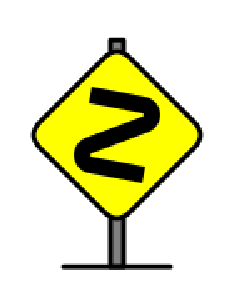
\includegraphics[height=1.3cm]{dbend.eps}
  \end{center}
\end{wrapfigure}
\noindent {\bf Perhatian:} Kesalahan umum ketika menggunakan indeks ialah
memakai modulus yang sama untuk indeks dan kongruensi asal. Padahal, ketika
kongruensi asal adalah modulo $n$, untuk $n\in\NN$, kongruensi indeks adalah
modulo $\phi(n)$!
\end{discussion}

\ifdefined\suppressallexercises
  {}
\else
  \vfill
  \pagebreak
  \subsection*{Latihan untuk \S\ref{sec:I}}
\fi

\begin{exercise}
Untuk modulus $n=17$, gunakan indeks untuk menyelesaikan kongruensi berikut:\newline
\hphantom{XXXXXXXXXXX}{\bf (a)}\ $4x\equiv11$\qquad\ {\bf (b)}\ $5x^6\equiv7$\qquad{\bf (c)}\ $x^{12}\equiv13$\newline
\hphantom{XXXXXXXXXXX}{\bf (d)}\ $8x^5\equiv10$\qquad{\bf (e)}\ $9x^8\equiv8$\qquad{\bf (f)}\ $7^x\equiv7$
\end{exercise}

\begin{exercise}
Aturan logaritma dalam Teorema~\ref{thm:indexprops} sangat mirip dengan aturan
logaritma biasa, tetapi satu aturan belum ada: rumus perubahan basis. Tentukan
bentuk rumus tersebut dalam konteks indeks, nyatakan secara formal, lalu
buktikan.
\end{exercise}

\begin{exercise}
Misalkan $p$ bilangan prima ganjil dan $a$ suatu akar primitif modulo $p$.
\begin{itemize}
\item[{\bf (a)}] Buktikan bahwa $\ind_a(-1)=(p-1)/2$.
\item[{\bf (b)}] Jika $x,y\in(\ZZ/p\ZZ)^*$ memenuhi $xy\equiv1\pmod{p}$,
apa hubungan antara $\ind_a(x)$ dan $\ind_a(y)$? Buktikan!
\item[{\bf (c)}] Jika $x,y\in(\ZZ/p\ZZ)^*$ memenuhi $x+y\equiv0\pmod{p}$,
apa hubungan antara $\ind_a(x)$ dan $\ind_a(y)$? Buktikan!
\end{itemize}
\end{exercise}

\vfill
\pagebreak
\ifdefined\boundarytwentysix
  \def\finishboundarytwentysix{\backmatter
    \bibliographystyle{amsalpha}
    \bibliography{refs}
    \printindex
    \end{document}}
\else
  \let\finishboundarytwentysix\relax
\fi
\finishboundarytwentysix
\section{Pertukaran Kunci Diffie--Hellman}
\label{sec:DHKE}
\begin{discussion}
Sekitar setahun sebelum kriptosistem RSA\index{RSA!kriptosistem} diciptakan,
Whitfield Diffie\index{Diffie, Whitfield} dan Martin
Hellman\index{Hellman, Martin} menerbitkan {\it New directions in cryptography}
\cite{diffie1976new}, uraian lengkap pertama dalam literatur ilmiah terbuka
mengenai kriptosistem kunci publik yang dapat berfungsi.\footnote{Sebenarnya,
beberapa bentuk kriptografi kunci publik yang dapat berfungsi telah ditemukan
lebih dahulu di lingkungan intelijen AS dan Britania Raya, tetapi tidak
dibagikan kepada publik. Sejak masa awal Perang Dingin, sejumlah pemerintahan
besar telah merahasiakan teorema dan bukti matematika.} Dalam makalah itu
mereka mendefinisikan sesuatu yang kemudian dinamai menurut keduanya:
\end{discussion}
\begin{definition}\label{def:DHKE}\index{pertukaran kunci Diffie--Hellman}
Protokol berikut disebut {\bf pertukaran kunci Diffie--Hellman} [{\bf DHKE}]:
\begin{enumerate}
\item Alice dan Bob menyepakati sebuah bilangan prima besar $p$ beserta akar
primitif\index{akar primitif} $r\in(\ZZ/p\ZZ)^*$, lalu mengumumkan keduanya.
\item Alice memilih $\alpha\in\ZZ$ yang memenuhi $2\le\alpha\le p-2$,
menghitung $A=r^\alpha\pmod{p}$, merahasiakan $\alpha$, tetapi mengumumkan $A$.
\item Bob memilih $\beta\in\ZZ$ yang memenuhi $2\le\beta\le p-2$,
menghitung $B=r^\beta\pmod{p}$, merahasiakan $\beta$, dan mengumumkan $B$.
\item Alice memperoleh nilai publik $B$ dan menghitung
$S=B^\alpha\pmod{p}$.
\item Bob memperoleh $A$ dan menghitung nilai yang sama,
$S=A^\beta\pmod{p}$.
\item Alice dan Bob memakai rahasia bersama $S$ sebagai kunci untuk komunikasi
selanjutnya, yang dienkripsi dengan suatu kriptosistem simetris yang telah
mereka sepakati sebelumnya.
\end{enumerate}
Nilai $S$ yang dimiliki Alice dan Bob [tetapi tidak dimiliki Eve] disebut
{\bf kunci bersama} atau {\bf rahasia bersama} mereka.
\end{definition}

\begin{discussion}
Gambaran grafisnya sebagai berikut:
\end{discussion}

\begin{center}
\resizebox{\textwidth}{!}{%
\begin{tabular}{|c|c|c|}
\multicolumn{3}{l}{\bf\ \ \ Pertukaran kunci Diffie--Hellman:}\\
\hline
Alice      &  di jaringan publik  & Bob\\
\hline
  &  pilih bilangan prima $p$ & \\
  &\ \   temukan akar primitif $r$\ \ & \\
\hline
pilih $\alpha$, hitung &  & pilih $\beta$, hitung\\
\ \ \ \ $A=r^\alpha\pmod{p}$\ \ \ \  & &\ \ \ \  $B=r^\beta\pmod{p}$\ \ \ \ \\
umumkan $A$ & $\rightarrowtail A$\quad\qquad$B\leftarrowtail$ & umumkan $B$\\
\hline
peroleh $B$, hitung &  & peroleh $A$, hitung\\
$S=B^\alpha\pmod{p}$  &  &  $S=A^\beta\pmod{p}$\\
\hline
\multicolumn{3}{|c|}{${}\xLeftrightarrow{\vphantom{\vec{X}}\text{\hphantom{XXXXXX}kriptografi simetris dengan kunci $S$\hphantom{XXXXXX}}}{}$}\\
\hline
\end{tabular}
}
\end{center}

\begin{proposition}\label{prop:DHKEworks}
Jika Alice dan Bob mengikuti protokol DHKE, keduanya menghitung kunci bersama
yang sama; \emph{dengan kata lain, DHKE berfungsi}.
\end{proposition}
\begin{proof}
Hanya sedikit yang perlu diperiksa. Dengan memakai notasi dalam definisi dan,
tepat di tengah, sifat komutatif perkalian, kita memperoleh
$$
B^\alpha \equiv \left(r^\beta\right)^\alpha
\equiv r^{\beta\cdot\alpha}\equiv r^{\alpha\cdot\beta}
\equiv\left(r^\alpha\right)^\beta\equiv A^\beta\pmod p\ .
$$
Ujung kiri kongruensi ini adalah $S$ yang dihitung Alice, sedangkan ujung
kanannya adalah $S$ yang dihitung Bob; keduanya sama sebagai kelas modulo $p$.
\end{proof}

\begin{example}
Dalam pembicaraan terbuka, Alice dan Bob sepakat memakai bilangan prima $p=617$
beserta akar primitifnya $r=17$.

Alice secara privat memilih nilai rahasianya $\alpha=19$ dan mengirim nilai
$$
A=17^{19}\equiv385\pmod{617}
$$
kepada Bob melalui surel yang tidak aman. (Tentu saja, setiap surel tanpa
enkripsi tidak aman.)

Bob memilih nilai rahasianya $\beta=13$ dan mengirim nilai
$$
B=17^{13}\equiv227\pmod{617}
$$
kepada Alice melalui surel yang tidak aman.

Alice menghitung rahasia bersama
$$
S=B^{\alpha}=227^{19}\equiv127\pmod{617}\ .
$$

Bob menghitung rahasia bersama yang sama melalui
$$
S=A^{\beta}=385^{13}\equiv127\pmod{617}\ .
$$

Mereka kemudian dapat memakai nilai ini sebagai kunci kriptografi simetris
untuk sisa komunikasi tersebut.
\end{example}

\begin{discussion}
Bagaimana dengan kepraktisan DHKE? Seperti dibahas dalam \S\ref{sec:tRSAC},
mencari bilangan prima [besar] $p$ (kita tetap memakai notasi dari
Definisi~\ref{def:DHKE}) layak secara komputasi,
\index{komputasi layak!digunakan} demikian pula beberapa eksponensiasi modular
\index{eksponensiasi modular cepat} dalam protokol DHKE. Masih tersisa persoalan
mencari akar primitif $r$.\index{akar primitif}

Salah satu caranya ialah menghindari pencarian $r$ lebih dari sekali. Setelah
satu bilangan prima $p$ beserta akar primitif $r$ modulo $p$ ditemukan, setiap
pengguna dapat memilih rahasianya sendiri ($\alpha$ milik Alice dan $\beta$
milik Bob) tanpa tumpang tindih atau konflik. Pendekatan ini disarankan dalam
sejumlah standar Internet; lihat, {\it misalnya,}
\cite{harkinsrfc} dan \cite{lepinski2008rfc}.

Strategi lain yang lebih matematis didasarkan pada definisi berikut. Kita
menyertakannya karena konsep ini menarik secara matematis dan tokoh yang
namanya diabadikan di dalamnya menjalani kehidupan yang luar biasa.
\end{discussion}
\begin{definition}\label{def:SGprime}\index{prima Sophie Germain!definisi}
Bilangan prima $p$ yang membuat $2p+1$ juga prima disebut
{\bf prima Sophie Germain}.
\end{definition}
\begin{discussion}

Belum diketahui berapa banyak prima Sophie Germain yang ada, meskipun diduga
jumlahnya tak hingga. Bahkan, terdapat dugaan yang cermat mengenai kepadatan
asimtotik prima semacam itu serta teknik algoritmik untuk membangkitkannya
secara efisien; lihat \cite{shoup2009computational}.
\end{discussion}
\begin{example}\index{prima Sophie Germain!contoh}
Tujuh belas prima Sophie Germain pertama ialah
\begin{center}
$2,\ 3,\ 5,\ 11,\ 23,\ 29,\ 41,\ 53,\ 83,\ 89,\ 113,\ 131,\ 173,\ 179,\ 191,\ 
233,\ 239$
\end{center}
Barisan semua prima Sophie Germain adalah barisan {\it A005384} dalam
{\it On-Line Encyclopedia of Integer Sequences}, {\tt oeis.org}.

Pada saat naskah sumber ini ditulis, prima Sophie Germain terbesar yang
diketahui ialah
\begin{center}
$18543637900515\times2^{666667}-1$
\end{center}
yang ditemukan pada 2012 oleh Philipp Bliedung dan sebuah jaringan besar
komputer terdistribusi.
\end{example}

\begin{discussion}
Kegunaan prima Sophie Germain dalam DHKE diselidiki pembaca melalui latihan di
bawah ini.

\vskip1mm
Seperti disebutkan dalam bagian sebelumnya~\ref{sec:I}, keamanan DHKE pada
keluarga parameter besar yang dipilih dengan sesuai bergantung pada asumsi
bahwa eksponensiasi modular berperilaku sebagai fungsi satu arah:\index{fungsi
satu arah} layak\index{komputasi layak!digunakan} dihitung ke arah maju (dengan
eksponensiasi modular cepat\index{eksponensiasi modular cepat}), tetapi belum
dikenal cara klasik yang layak untuk membalik operasi itu (yakni menghitung
suatu indeks).

Jika logaritma diskret dapat dihitung dengan algoritme layak, Eve dapat
membobol DHKE sepenuhnya. Berawal dari nilai publik $A$ dan $B$, ia
akan menghitung $\alpha=\ind_r(A)$ dan $\beta=\ind_r(B)$. Selanjutnya ia dapat
menghitung $S$ sebagai $B^\alpha$, $A^\beta$, atau langsung sebagai
$r^{\alpha\cdot\beta}$. Setelah memperoleh $S$, ia dapat mendekripsi komunikasi
Alice dan Bob yang lewat.

Sebenarnya, Eve tidak harus mampu menghitung logaritma diskret selama ia dapat
menyelesaikan suatu masalah komputasi tertentu.
\end{discussion}
\begin{definition}\label{def:DHproblem}\index{masalah Diffie--Hellman}
{\bf Masalah Diffie--Hellman} [{\bf DHP}] adalah pertanyaan berikut. Diberikan
\begin{itemize}
\item bilangan prima $p$,
\item akar primitif $r\in(\ZZ/p\ZZ)^*$, dan
\item dua unsur $a,b\in(\ZZ/p\ZZ)^*$ yang diketahui berbentuk $a=r^x$ dan
$b=r^y$ untuk $x,y\in\NN$, meskipun $x$ dan $y$ tidak diketahui,
\end{itemize}
hitung
\begin{itemize}
\item $r^{xy}$\ .
\end{itemize}
\end{definition}
\begin{discussion}
Cara efisien untuk menghitung logaritma diskret tentu menghasilkan penyelesaian
DHP. Namun, belum diketahui apakah DHP dapat diselesaikan tanpa
algoritme lengkap untuk menghitung logaritma diskret. Karena pertanyaan ini
masih terbuka pada saat naskah sumber ditulis, pernyataan yang paling cermat
ialah bahwa membobol DHKE berarti menyelesaikan DHP. Untuk keluarga parameter
besar yang dipilih dengan sesuai, tidak dikenal algoritme klasik yang layak
untuk melakukannya.\footnote{Seperti pada faktorisasi, terdapat algoritme yang
diketahui untuk {\it komputer kuantum}\index{komputer kuantum} yang
menyelesaikan DHP secara efisien; lihat \cite{shor1994algorithms}.}

\vskip1mm
DHKE merupakan salah satu protokol kriptologi yang paling luas digunakan di
Internet. Protokol ini atau variannya dipakai, antara lain, dalam SSL, TLS, SSH,
IPsec, dan banyak VPN.
\end{discussion}

\ifdefined\suppressallexercises
  {}
\else
  \vfill
  \pagebreak
  \subsection*{Latihan untuk \S\ref{sec:DHKE}}
\fi

\begin{exercise}
Andaikan Anda mempunyai algoritme efisien untuk membangkitkan prima Sophie
Germain yang besar. Jelaskan cara memakainya untuk memilih parameter publik
awal DHKE: telusuri semua tahap penyiapan protokol ini dan jelaskan bagaimana
setiap tahap dapat dilakukan {\it secara layak}\index{komputasi
layak!digunakan}, berdasarkan pembahasan terdahulu tentang perhitungan yang
dapat kita lakukan secara layak atau berdasarkan gagasan baru yang Anda
kembangkan di sini.
\end{exercise}

\begin{exercise}\label{exc:DHKEcomputation}
Bilangan $p=11717$ adalah prima dan $r=103$ merupakan akar primitif modulo $p$.
Dengan berperan sebagai Alice, % dengan $\alpha=71$
pengajar Anda telah menghitung $A=5123$.

Berperanlah sebagai Bob dan lakukan apa yang diperlukan untuk membentuk kunci
bersama dengan pengajar Anda: hitung $S$ seperti dalam DHKE dan kirimkan $B$
Anda melalui surel agar pengajar juga dapat menghitung $S$. Kemudian tunggu
petunjuk lanjutan melalui surel balasan yang dienkripsi dengan rahasia bersama.

Anda mungkin perlu melakukan perhitungan yang sulit dikerjakan dengan
kalkulator genggam. Jika Anda memiliki akses ke dan terbiasa dengan sistem
komputer seperti {\tt Octave, Matlab}, atau {\tt Mathematica}, perhitungan ini
dapat dilakukan dengan sistem tersebut. Jika tidak, cobalah mencari frasa
``fast modular exponentiation applet'' dengan mesin pencari favorit Anda atau
memakai {\tt wolframalpha.com}.
\end{exercise}

\begin{exercise}
Uraikan dengan perincian matematis yang cermat semua langkah yang digunakan
dalam serangan man-in-the-middle terhadap DHKE.
\end{exercise}

\vfill
\pagebreak
\ifdefined\boundarytwentyseven
  \def\finishboundarytwentyseven{\backmatter
    \bibliographystyle{amsalpha}
    \bibliography{refs}
    \printindex
    \end{document}}
\else
  \let\finishboundarytwentyseven\relax
\fi
\finishboundarytwentyseven
\section{Kriptosistem ElGamal}
\label{sec:tEGC}
\begin{discussion}
Seperti disebutkan dalam bagian sebelumnya, untuk keluarga parameter besar yang
dipilih dengan sesuai, eksponensiasi modulo bilangan prima publik $p$ merupakan
calon fungsi satu arah\index{fungsi satu arah} yang baik. Perhitungan ke arah
maju berlangsung cepat (layak),\index{komputasi layak!digunakan} sedangkan
inversnya, yakni logaritma diskret\index{logaritma diskret} relatif terhadap
akar primitif\index{akar primitif} $r$ modulo $p$, belum diketahui dapat
dihitung dengan algoritme klasik yang layak---bahkan ketika akar itu diketahui
publik. Asumsi ini mendasari DHKE\index{pertukaran kunci Diffie--Hellman}; kini
kita membahas cara memakai gagasan satu arah tersebut untuk membentuk
kriptosistem kunci publik yang lebih lazim, yaitu kriptosistem ElGamal.

Dalam kriptosistem kunci publik RSA, enkripsi dilakukan dengan eksponensiasi
modulo $n=pq$. Dekripsi kemudian dilakukan dengan eksponen yang merupakan
invers multiplikatif eksponen enkripsi modulo $\phi(n)$. Pemilik kunci privat,
yang mengetahui faktor rahasia $p$ dan $q$, juga dapat mengetahui eksponen
dekripsi karena ia dapat menghitung $\phi(n)$.

Dengan cara serupa, ElGamal memakai operasi aritmetika elementer---mengalikan
bentuk numerik pesan dengan suatu faktor pengacak modulo bilangan tertentu---
untuk melakukan pengacakan yang diperlukan dalam enkripsi. Cipherteks membawa
informasi secukupnya agar penerima yang dituju, yang mengetahui nilai logaritma
diskret tertentu, dapat membatalkan perkalian pengacak itu. Berikut rinciannya.
Konstruksi buku teks ini menetapkan cara kerja dan kebenaran fungsionalnya;
jaminan keamanan yang lebih kuat memerlukan asumsi mengenai grup, pembangkitan
parameter, enkode, dan keacakan baru yang independen yang tidak dibuktikan di sini.
\end{discussion}
\begin{definition}\label{def:ElGamalcrypto}\index{kriptosistem ElGamal}
Untuk memulai, Alice memilih bilangan prima besar $p$, akar primitif $r$ modulo
$p$, dan nilai rahasia $\alpha\in\NN$ yang memenuhi
$2\le\alpha\le p-2$. Ia menghitung $a=r^\alpha\pmod p$, lalu memasang
{\bf kunci publik} [{\bf enkripsi}] {\bf ElGamal} miliknya, yaitu $(p,r,a)$,
di situs webnya.

{\bf Kunci privat} [{\bf dekripsi}] {\bf ElGamal} milik Alice adalah
$(p,r,\alpha)$. Hubungan kunci dekripsi dengan kunci enkripsi diberikan oleh
$\Ee:(p,r,\alpha)\mapsto(p,r,r^\alpha\pmod*{p})$.

Ruang pesannya ialah $\Mm=\{m\in\ZZ\mid 2\le m\le p-1\}$. Kita menganggap
setiap unsurnya dapat ditafsirkan sebagai pesan bermakna yang dienkode secara
numerik dengan suatu skema yang dikenal luas.

Misalkan Bob ingin mengirim plainteks $m\in\Mm$ kepada Alice. Untuk setiap
pesan baru $m$, ia membangkitkan bilangan acak baru $\beta\in\NN$ yang
memenuhi $2\le\beta\le p-2$, lalu membentuk cipherteks untuk
{\bf enkripsi ElGamal}, yang terdiri atas dua komponen
$$
c=e_{(p,r,a)}(m)=(r^\beta\pmod*{p},\ m\cdot a^\beta\pmod*{p})\ .
$$

Ketika menerima cipherteks $c=(c_1,c_2)$, Alice dapat memulihkan plainteks
dengan {\bf dekripsi ElGamal}
$$
d_{(p,r,\alpha)}(c_1,c_2)
=c_2\cdot c_1^{p-1-\alpha}\pmod p\ .
$$

Semua komponen di atas bersama-sama membentuk
{\bf kriptosistem ElGamal}.
\end{definition}
\begin{discussion}

Pertama-tama, kita perlu memastikan bahwa konstruksi ini benar dalam arti
berikut.
\end{discussion}
\begin{proposition}\label{prop:ElGamalcryptocorrect}
Dengan notasi dalam Definisi~\ref{def:ElGamalcrypto}, berlaku
$$
d_{(p,r,\alpha)}(e_{(p,r,a)}(m)) = m\quad\forall m\in\Mm\ .
$$
\end{proposition}
\begin{proof}
Cukup lakukan perhitungan berikut:
\begin{align*}
d_{(p,r,\alpha)}(e_{(p,r,a)}(m))
&\equiv m\cdot a^\beta\cdot(r^\beta)^{p-1-\alpha}\pmod{p}\\
&\equiv m\cdot (r^\alpha)^\beta\cdot(r^\beta)^{p-1-\alpha}\pmod{p}\\
&\equiv m\cdot r^{\alpha\beta+\beta(p-1)-\alpha\beta}\pmod{p}\\
&\equiv m\cdot (r^{p-1})^\beta\pmod{p}\\
&\equiv m\cdot 1^\beta\pmod{p}\\
&\equiv m\pmod{p}
\end{align*}
Perhatikan bahwa eksponen $p-1-\alpha$ pada suku $c_1$ dalam dekripsi
menghasilkan $(c_1^{-1})^\alpha$ tanpa memakai pangkat negatif, berdasarkan
Teorema~\ref{thm:powersinmodordna}.
\end{proof}

\begin{discussion}
Secara grafis:
\end{discussion}

\begin{center}
\resizebox{\textwidth}{!}{%
\begin{tabular}{|c|c|c|}
\multicolumn{3}{l}{\bf\ \ \ Kriptosistem ElGamal:}\\
\hline
Alice      &  di jaringan publik  & Bob\\
\hline
pilih bilangan prima $p$  &  & \\
temukan akar primitif $r$ & & \\
pilih $\alpha\ \mid\ 2\le\alpha\le p-2$ & & \\
hitung $a=r^\alpha\pmod{p}$ & &\\
umumkan kunci publik &\ \ \ \  $\rightarrowtail(p,r,a)$\ \ \ \ \ \ \ \  \ &
unduh kunci publik\\
\hline
& & diberi pesan $m\in\Mm$ \\
& & (jadi $2\le m\le p-1$) \\
& & pilih $\beta\ \mid\ 2\le\beta\le p-2$ \\
& & hitung $c_1=r^\beta\pmod*{p}$\\
& & dan $c_2=m\cdot a^\beta\pmod*{p}$\\
terima cipherteks&\ \ \ \ \ \ $(c_1,c_2)\leftarrowtail$ & kirim cipherteks\\
\hline
hitung plainteks &  & \\
$m\equiv c_2\cdot c_1^{p-1-\alpha}\pmod p$ & &\\
\hline
\end{tabular}
}
\end{center}

\begin{discussion}
\vskip6mm
ElGamal juga memiliki algoritme tanda tangan digital yang menarik:
\end{discussion}
\begin{definition}\label{def:ElGamalsig}\index{tanda tangan digital!ElGamal}
Misalkan Alice memiliki kunci privat ElGamal $(p,r,\alpha)$ dan ingin
menandatangani pesan $m\in\Mm$ secara digital. Untuk setiap tanda tangan baru,
mula-mula ia memilih $\gamma\in\NN$ secara acak sehingga
$1<\gamma<p-1$ dan
$\gcd(\gamma,p-1)=1$.\index{faktor persekutuan terbesar!digunakan}

Tuliskan $x=r^\gamma\pmod*{p}$ dan
$y=\gamma^{-1}\cdot(m-\alpha x)\pmod*{p-1}$, dengan invers diambil modulo
$p-1$. Tanda tangan digital pada $m$ ialah pasangan $(x,y)$.

Untuk memverifikasi tanda tangan $(x,y)$ pada pesan $m$ dengan kunci publik
Alice $(p,r,a)$, Bob memeriksa apakah
$a^x\cdot x^y\equiv r^m\pmod{p}$. Jika ya, ia menerima; jika tidak, ia menolak.
\end{definition}
\begin{discussion}

Sekali lagi, kita ingin memastikan bahwa prosedur ini memberikan hasil yang
semestinya.
\end{discussion}
\begin{proposition}\label{prop:ElGamalsigcorrect}
Dengan notasi di atas, Bob akan menerima setiap pesan bertanda tangan yang
dihasilkan Alice menurut prosedur tersebut.
\end{proposition}
\begin{proof}
Andaikan pesan bertanda tangan $(m,x,y)$ dibuat Alice seperti di atas. Karena
$y\equiv\gamma^{-1}(m-\alpha x)\pmod{p-1}$, kita mempunyai
$\gamma y\equiv m-\alpha x\pmod{p-1}$. Dengan
Teorema~\ref{thm:powersinmodordna}, kita menghitung
\begin{align*}
a^x\cdot x^y &\equiv (r^\alpha)^x\cdot(r^\gamma)^y\pmod{p}\\
&\equiv r^{\alpha x+\gamma y}\pmod{p}\\
&\equiv r^{\alpha x+(m-\alpha x)}\pmod{p}\\
&\equiv r^m\pmod{p}
\end{align*}
Jadi, Bob akan menerima tanda tangan tersebut.
\end{proof}

\begin{discussion}
Secara grafis:
\end{discussion}

\begin{center}
\resizebox{\textwidth}{!}{%
\begin{tabular}{|c|c|c|}
\multicolumn{3}{l}{\bf\ \ \ Tanda tangan digital ElGamal:}\\
\hline
Alice  & di jaringan publik &  Bob\\
\hline
temukan bilangan prima $p$ dan & & \\
akar primitif $r$ & & \\
pilih $\alpha\ \mid\ 2\le\alpha\le p-2$ & & \\
hitung $a=r^\alpha\pmod{p}$ & & \\
umumkan kunci publik & $\rightarrowtail(p,r,a)$\ \ \ \ \ \ \ \  & unduh kunci
publik\\
\hline
diberi pesan $m\in\Mm$ & & \\
(jadi $2\le m\le p-1$) & & \\
pilih $\gamma$ acak dengan $1<\gamma<p-1$ & & \\
dan $\gcd(\gamma,p-1)=1$ & & \\
hitung $s_1=r^\gamma\pmod*{p}$ dan & & \\
$s_2=\gamma^{-1}\cdot(m-\alpha s_1)\pmod*{p-1}$ & &\\
kirim pesan bertanda tangan & $\rightarrowtail(m,s_1,s_2)$ & terima pesan bertanda tangan\\
\hline
& & \ \ jika $a^{s_1}\cdot s_1^{s_2}\equiv r^m\pmod*{p}$\\
& & {\sc terima}\qquad\  \\
& & jika tidak,\qquad\qquad\quad\  \\
& & {\sc tolak}\qquad\  \\
\hline
\end{tabular}
}
\end{center}

\ifdefined\suppressallexercises
  {}
\else
  \vfill
  \pagebreak
  \subsection*{Latihan untuk \S\ref{sec:tEGC}}
\fi

\begin{exercise}\label{exc:ElGcomputation}
Pengajar Anda masih menyukai bilangan prima $p=11717$ dengan akar primitif
$r=103$ dari latihan terdahulu~\ref{exc:DHKEcomputation} tentang DHKE. Selain
itu, pengajar telah menghitung nilai $a=1020$ %bersesuaian dengan \alpha=666
untuk melengkapi kunci publik ElGamal
$(p,r,a)=(11717,103,1020)$.

Dengan kunci publik ini, Anda ingin mengirim pesan berupa bilangan 42 kepada
pengajar (bagaimanapun, itulah jawaban atas ``kehidupan, alam semesta, dan
segala sesuatu''). Cipherteks apa yang akan Anda kirim? Tunjukkan perhitungan
Anda!
\end{exercise}

\begin{exercise}
Sekarang pengajar ingin mengirimkan nilai ujian terbaru Anda melalui surel.
Untuk mendukung klaim bahwa surel itu benar-benar berasal dari pengajar, surel
tersebut memuat nilai 97 beserta tambahan: ``Nilai ini ditandatangani dengan
tanda tangan digital ElGamal memakai kunci publik saya [kunci publik pengajar
yang sama seperti dalam Latihan~\ref{exc:ElGcomputation}, yaitu
$(p,r,a)=(11717,103,1020)$]; nilai tanda tangannya adalah $(6220,10407)$.''

Apakah tanda tangan itu lolos verifikasi? Dengan asumsi pengikatan
identitas--kunci pengajar telah diautentikasi dan kunci privatnya tidak terkompromi,
apakah Anda menerima surel tersebut sebagai benar-benar berasal dari pengajar?
Tunjukkan perhitungan Anda!
% memakai \gamma=23 sehingga \gamma^{-1}=2547 (modulo 11716)
\end{exercise}

\begin{exercise}
Buat kunci publik ElGamal dan kirimkan kepada pengajar melalui surel. Tunggu
pesan balasan yang dienkripsi dengan ElGamal, lalu kirim kembali plainteksnya
kepada pengajar.

Selain itu, gunakan kunci publik Anda untuk menandatangani bilangan 17 sebagai pesan.
Kirimkan bilangan bertanda tangan itu kepada pengajar dan tunggu kabar apakah
tanda tangannya diterima atau ditolak.
\end{exercise}

\ifdefined\boundarytwentyeight
  \def\finishboundarytwentyeight{\backmatter
    \bibliographystyle{amsalpha}
    \bibliography{refs}
    \printindex
    \end{document}}
\else
  \let\finishboundarytwentyeight\relax
\fi
\finishboundarytwentyeight

\backmatter

\ifdefined\suppressBibliography
  {}
\else
  \bibliographystyle{amsalpha}
  \bibliography{refs}
\fi

\ifdefined\suppressIndex
  {}
\else
  \printindex
\fi

\end{document}

%
% To do:
%  1) Add many, many more examples, such as of encryption with various
%     cryptosystems using both toy, small keys and full sized ones; also of
%     the theorems about multiplicative order, for example.
%  2) Include Octave code to do various crypto and number theoretic tasks.
%  3) More references to other readings, such as to historical origins
%     and to websites with crypto discussions and software.
%  4) Make sure the text has all relevant index entries.
%  5) Insert the dbend symbol everywhere relevant.
%  6) Do an example of an index solution to a monomial congruence where one of
%     of the terms is not invertible in mod $\phi(n)$
%
